\section{Transfer learning}

\begingroup
\setbeamertemplate{navigation symbols}{}  % remove page number within the group
\begin{frame}[noframenumbering]{}
    \centering
    \vspace{3cm}
    \Huge
    \textcolor{myblue}{Transfer learning from experimental setup to operational data}
\end{frame}
\endgroup

\subsection{Context}

\begin{frame}{Context}{Experimental vs. operational}
    
    \renewcommand{\ratio}{0.9}
    \begin{overprint}
        \onslide<1>\centering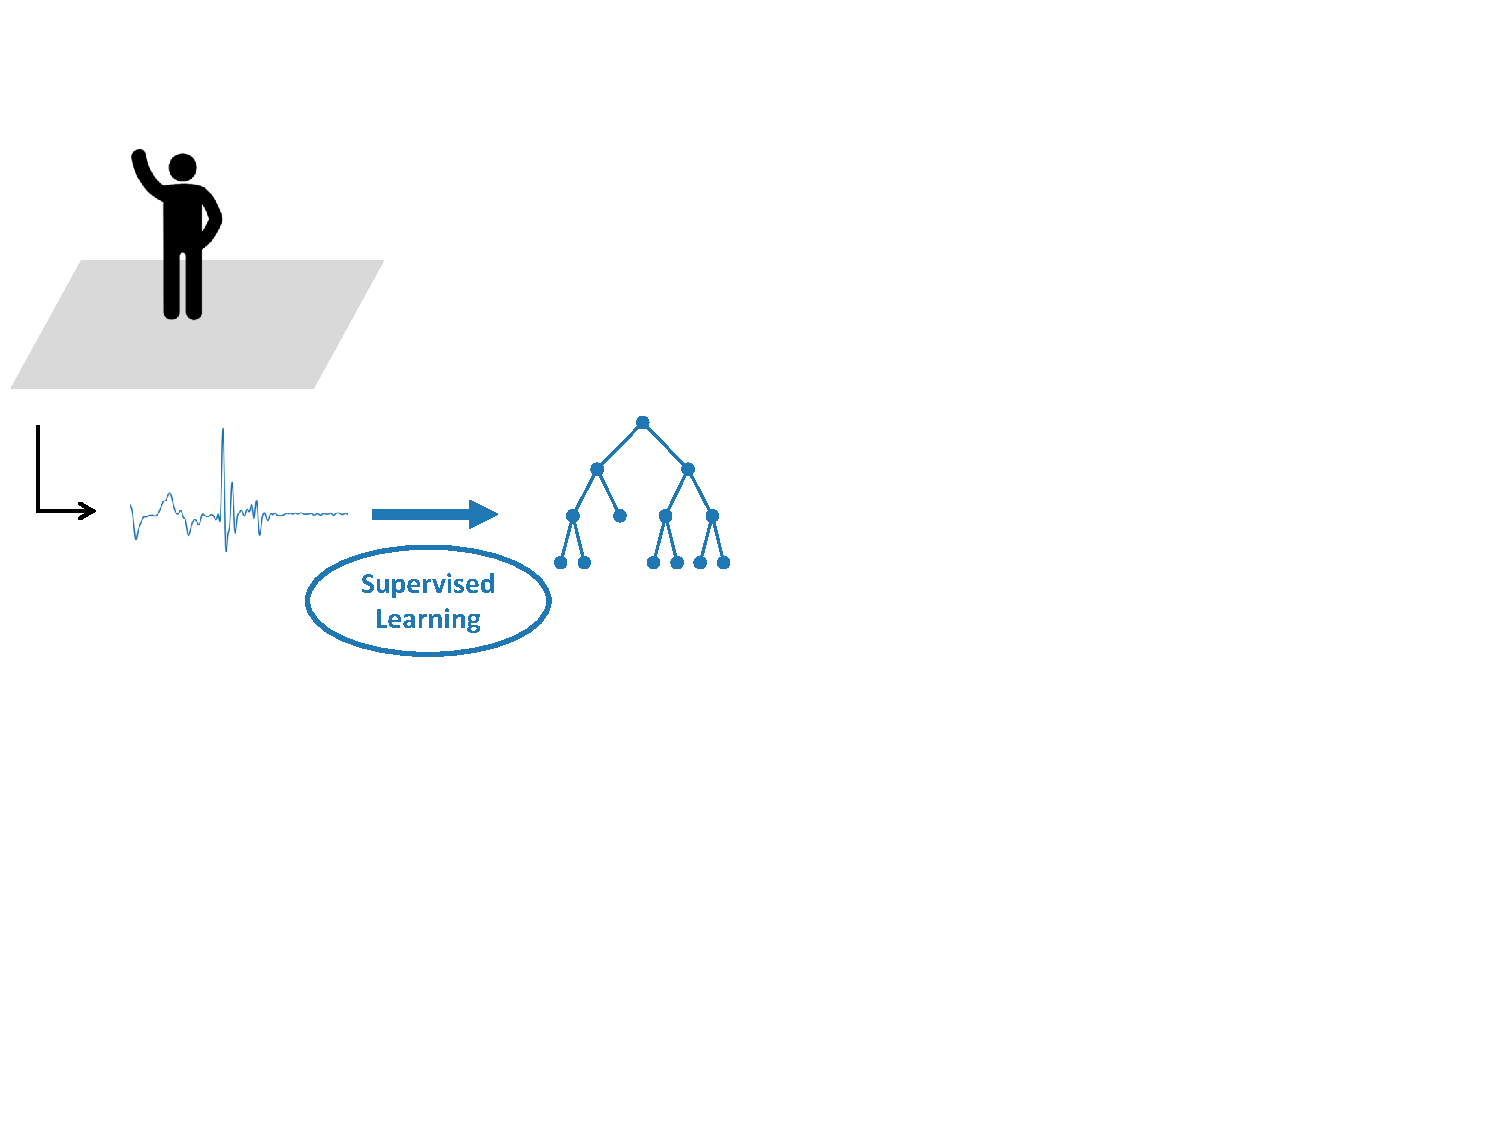
\includegraphics[width=\ratio\linewidth,trim={0 20 0 60},clip]{schemas_tl_1.pdf}
        \onslide<2>\centering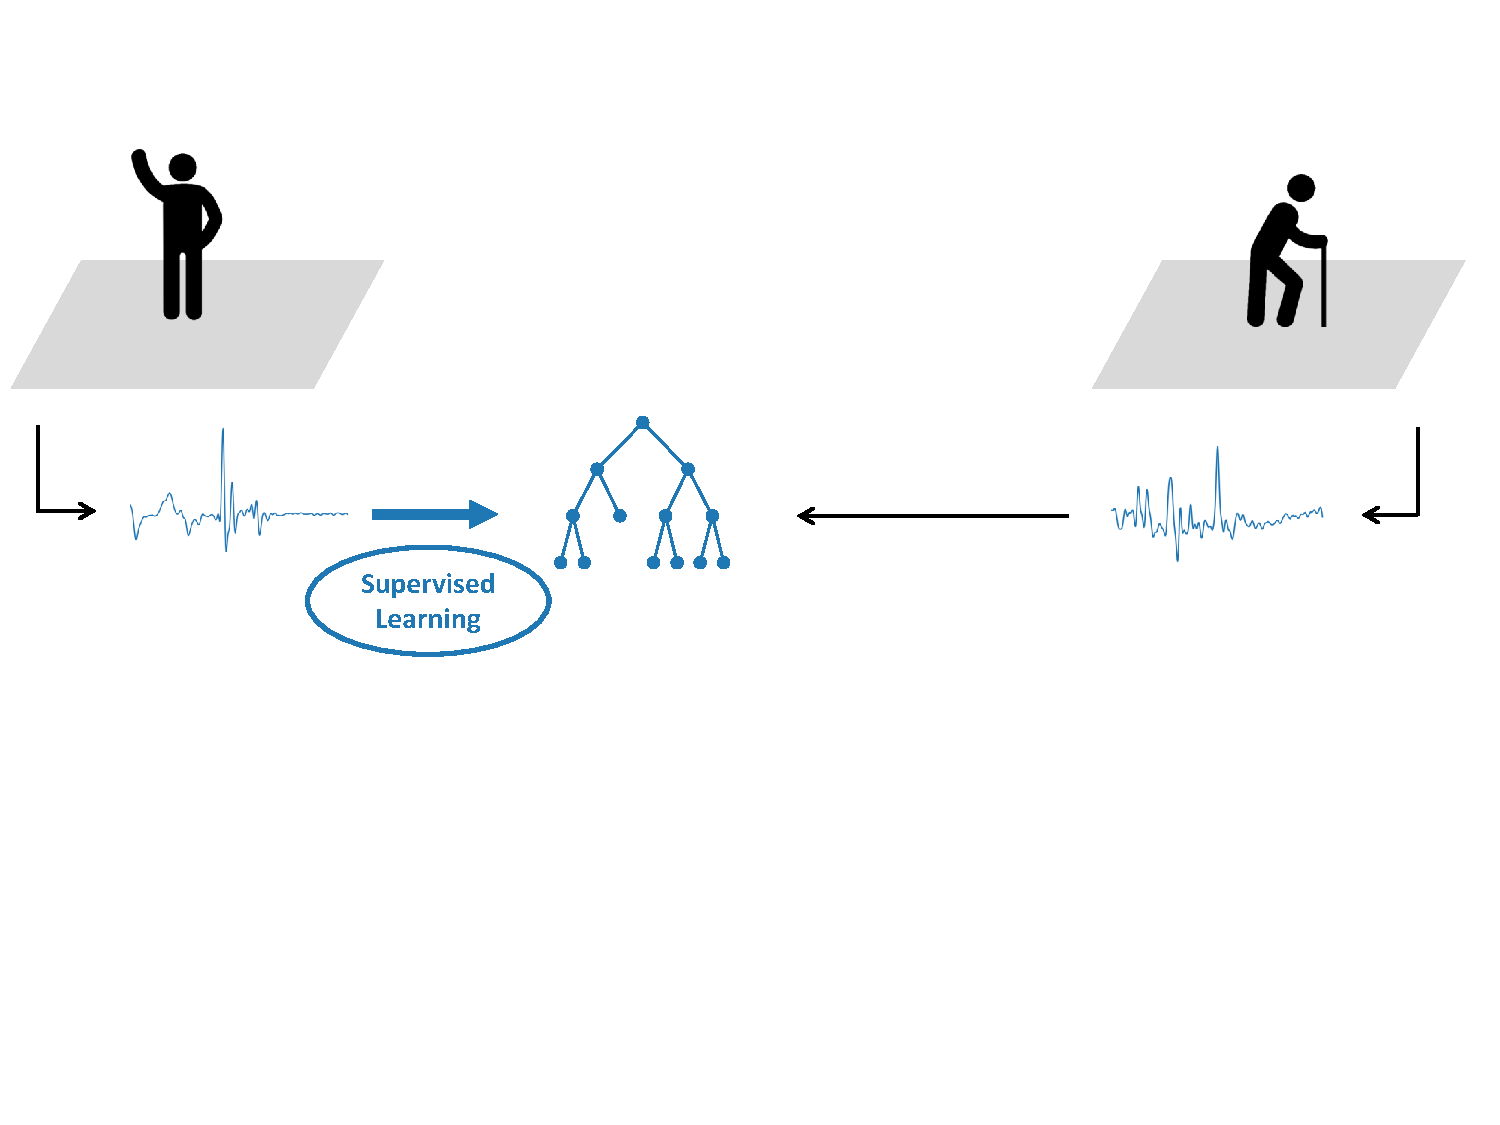
\includegraphics[width=\ratio\linewidth,trim={0 20 0 60},clip]{schemas_tl_2.pdf}
        \onslide<3>\centering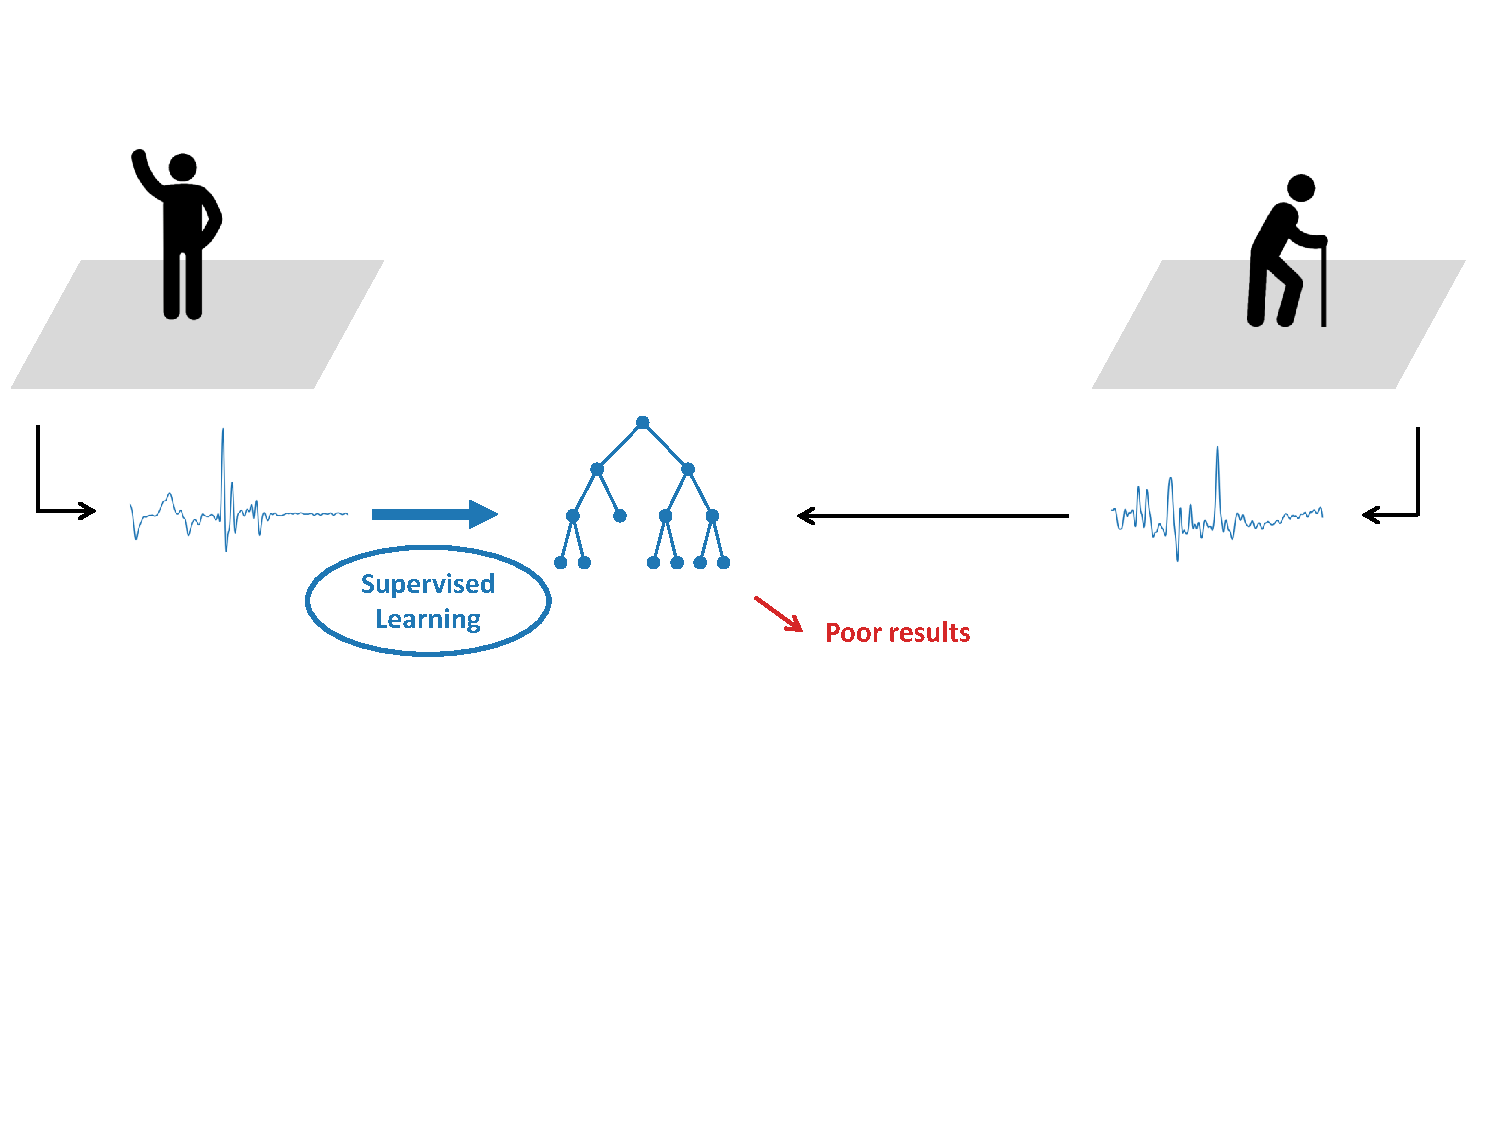
\includegraphics[width=\ratio\linewidth,trim={0 20 0 60},clip]{schemas_tl_3.pdf}
%         \onslide<4>\centering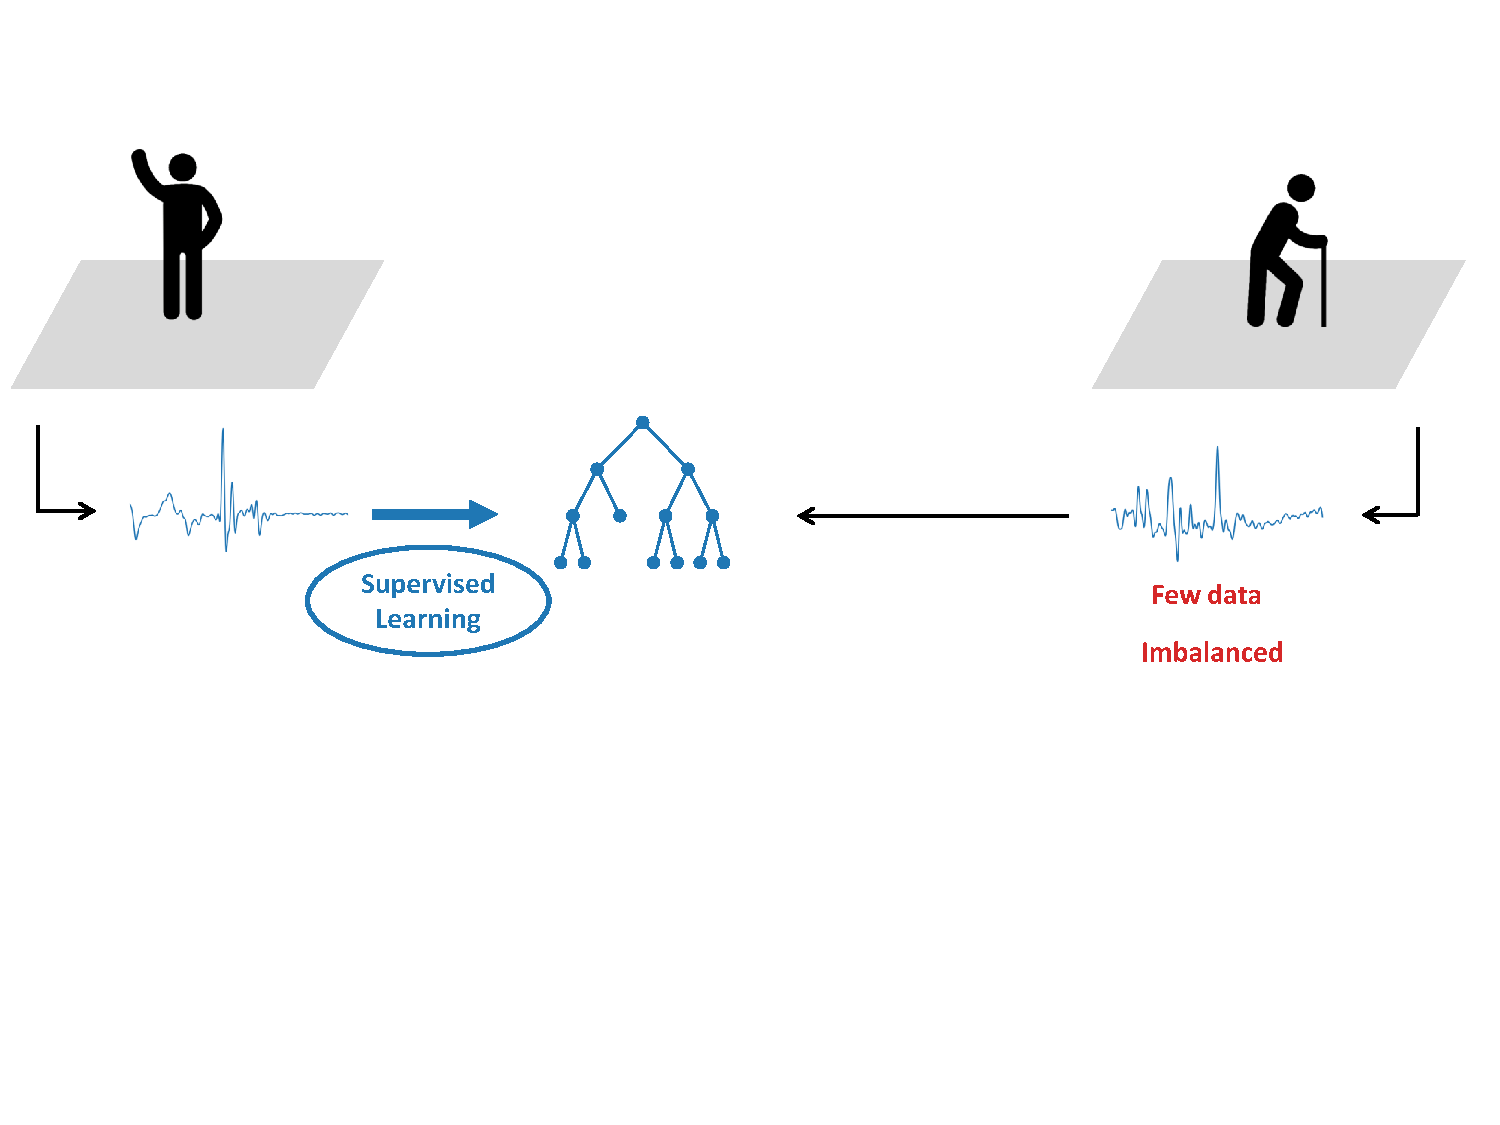
\includegraphics[width=\ratio\linewidth,trim={0 20 0 60},clip]{schemas_tl_4.pdf}
        \onslide<4>\centering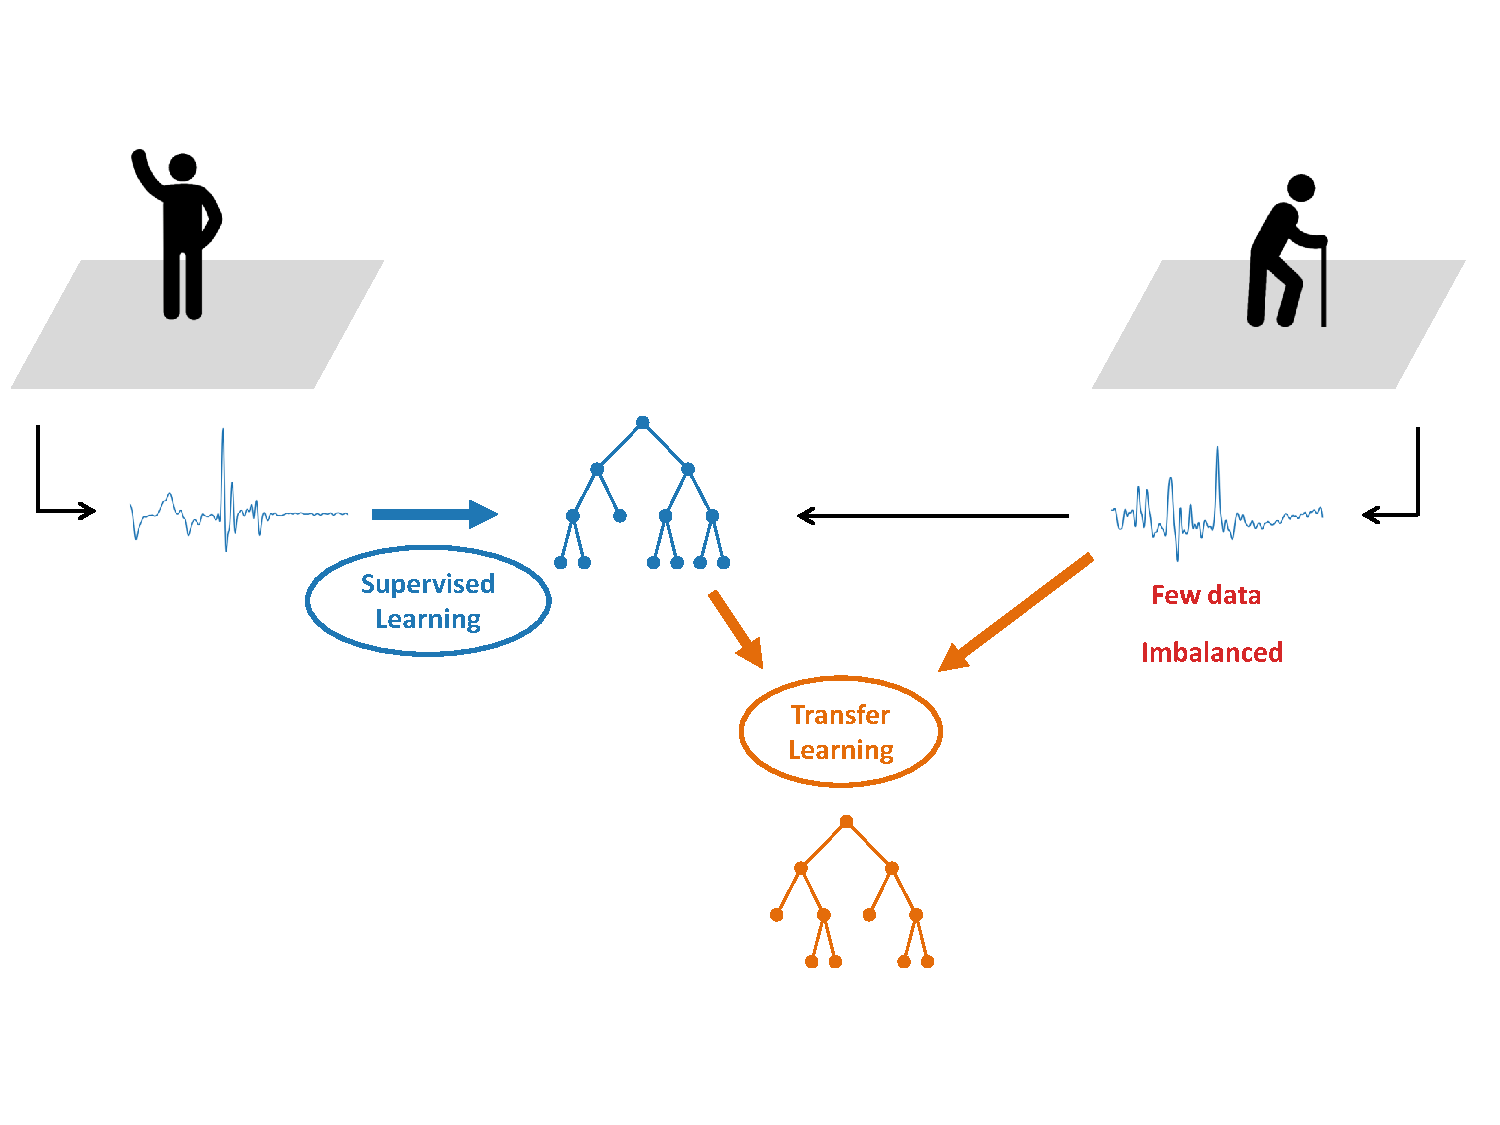
\includegraphics[width=\ratio\linewidth,trim={0 20 0 60},clip]{schemas_tl_5.pdf}
    \end{overprint}

\end{frame}


\begin{frame}{Context}{Transfer learning}
\begin{minipage}[t]{0.49\linewidth}
    \vspace{0pt}
    \textbf{Transfer learning}
    \begin{itemize}
        \item Source domain: $\mathcal{D}_{S} = \{\mathcal{X}_{S}, P(X_{S})\}$\\
        \item Target domain: $\mathcal{D}_{T} = \{\mathcal{X}_{T}, P(X_{T})\}$\\
        \item Source task: $\mathcal{T}_{S} = \{\mathcal{Y}_{S}, f^S\}$\\
        \item Target task: $\mathcal{T}_{T} = \{\mathcal{Y}_{T}, f^T\}$\\
    \end{itemize}
\end{minipage}
\begin{minipage}[t]{0.49\linewidth}
    \vspace{0pt}
    \textbf{Our case}
    \begin{itemize}%[label=$\bullet$]
        \item $\mathcal{X}_{S} = \mathcal{X}_{T}$
        \item \textcolor{myorange}{$P(X_{S}) \neq P(X_{T})$}
        \item $\mathcal{Y}_{S} = \mathcal{Y}_{T}$
        \item \textcolor{myorange}{$f^S \neq f^T$}
    \end{itemize}
\end{minipage}

\bigskip

\renewcommand{\ratio}{0.32}
\centering
\begin{minipage}[t]{0.85\linewidth}
    \centering
    \begin{minipage}[t]{\ratio\linewidth}
        \centering
        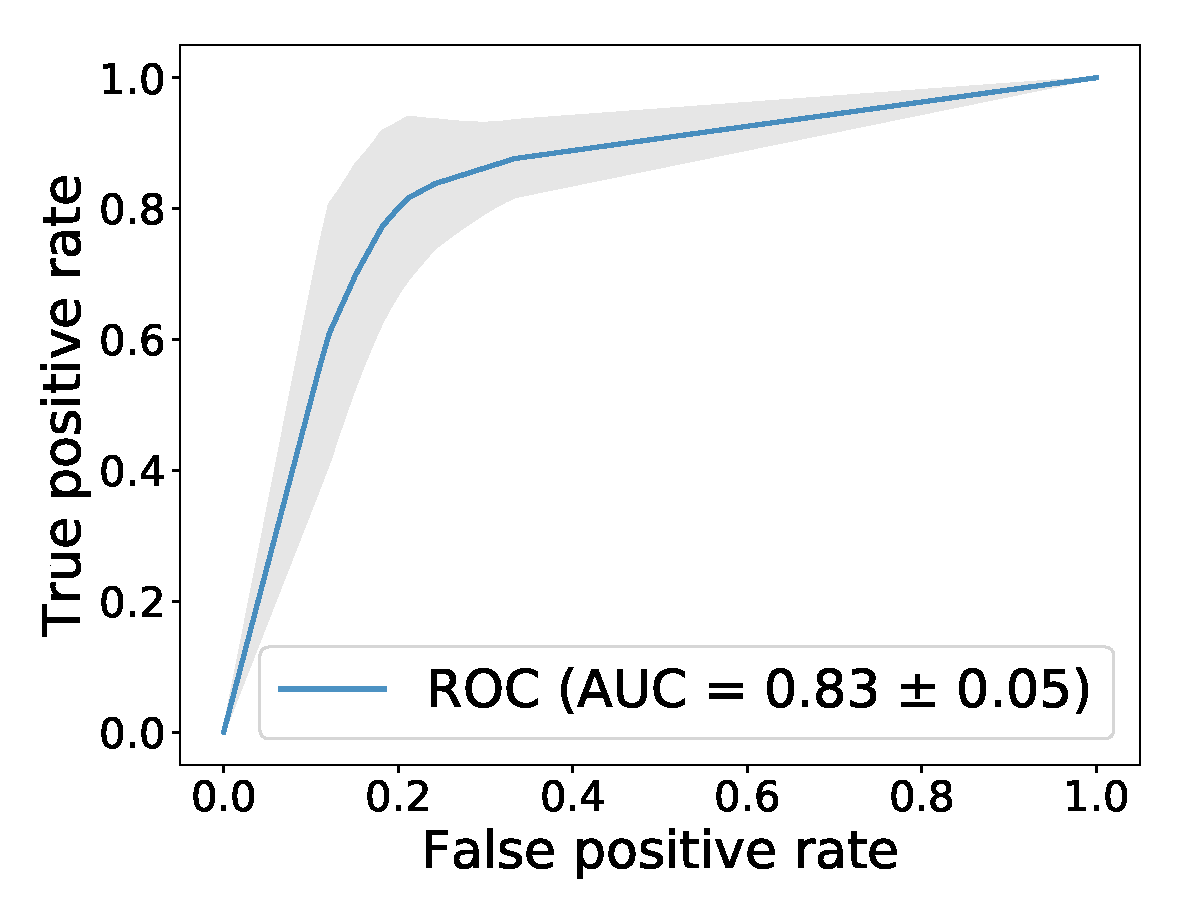
\includegraphics[width=\linewidth]{kfold_10_ntree_1_featmat_base_ech1nb_feat_872019_11_25RF_Source_On_Source_ROC.pdf}\\
        {\small \emph{Source} tested on source}
    \end{minipage}
    \begin{minipage}[t]{\ratio\linewidth}
        \centering
        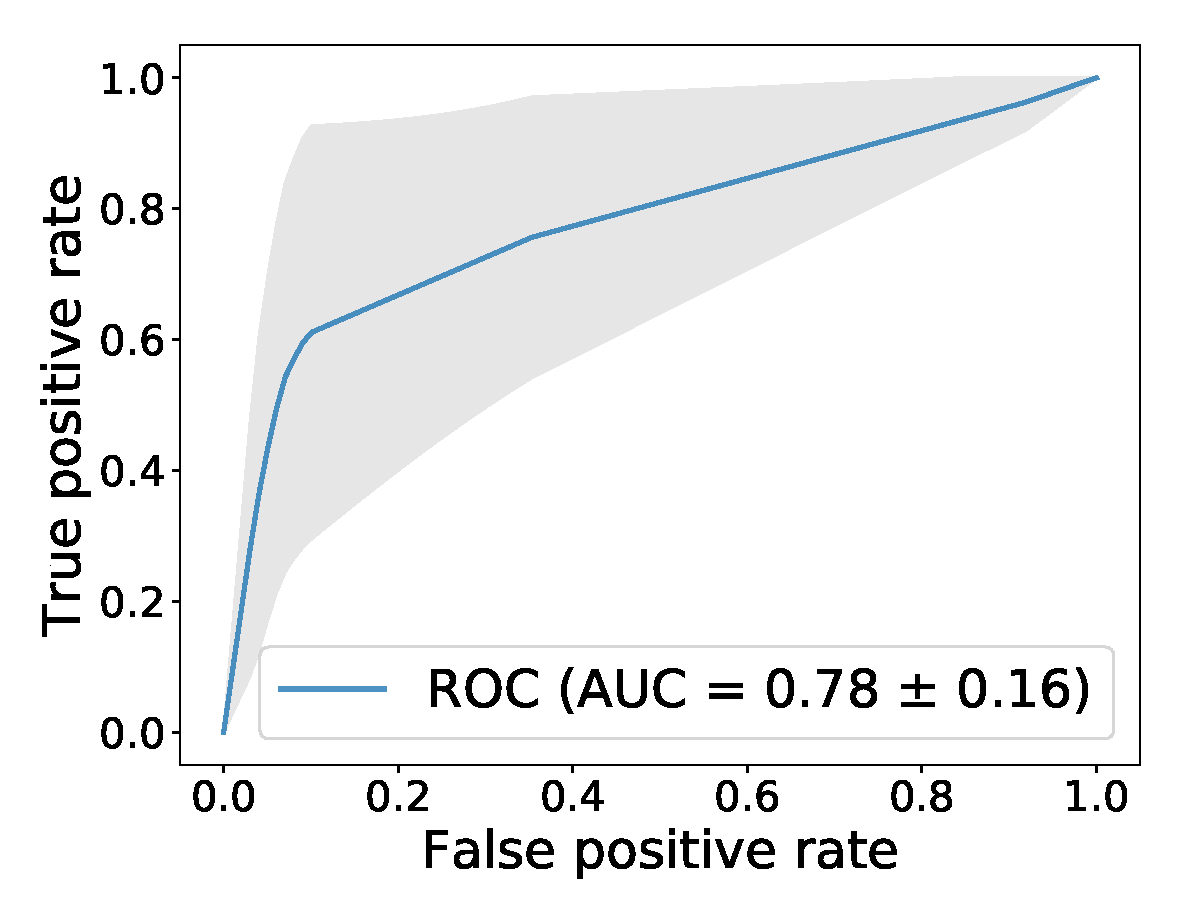
\includegraphics[width=\linewidth]{kfold_10_ntree_1_featmat_base_ech1nb_feat_872019_11_25RF_Source_On_Target_ROC_2.pdf}\\
        {\small \emph{Source} tested on target}
    \end{minipage}
    \begin{minipage}[t]{\ratio\linewidth}
        \centering
        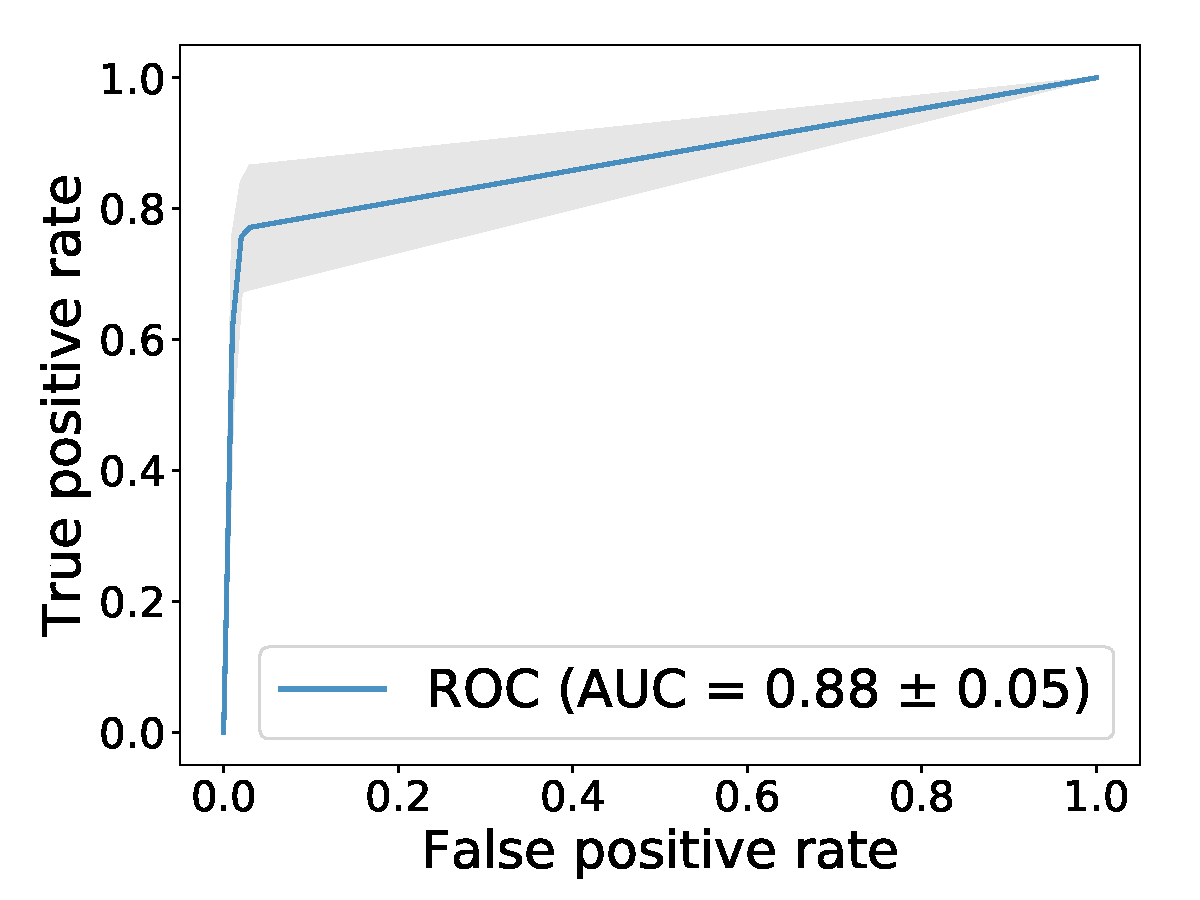
\includegraphics[width=\linewidth]{kfold_10_ntree_1_featmat_base_ech1nb_feat_872019_11_25RF_Target_On_Target_ROC.pdf}\\
        {\small \emph{Target} tested on target}
    \end{minipage}
\end{minipage}

\begin{itemize}
    \item \textbf{Goal}: Use knowledge from source and target domains to improve the final task while avoiding \textit{negative transfer}
    \item Model-based transfer: we have access to the Source model and target data
\end{itemize}


\end{frame}

\subsection{Model-based transfer}

\begin{frame}{Model-based transfer}

\centering\citet{segev2017learn}

\begin{minipage}[t]{0.49\linewidth}
    \vspace{0pt}
    \centering
    \textbf{Structure Expansion / Reduction (SER)}
    
    \renewcommand{\ratio}{0.55}
%     \begin{overprint}
%         \onslide<1>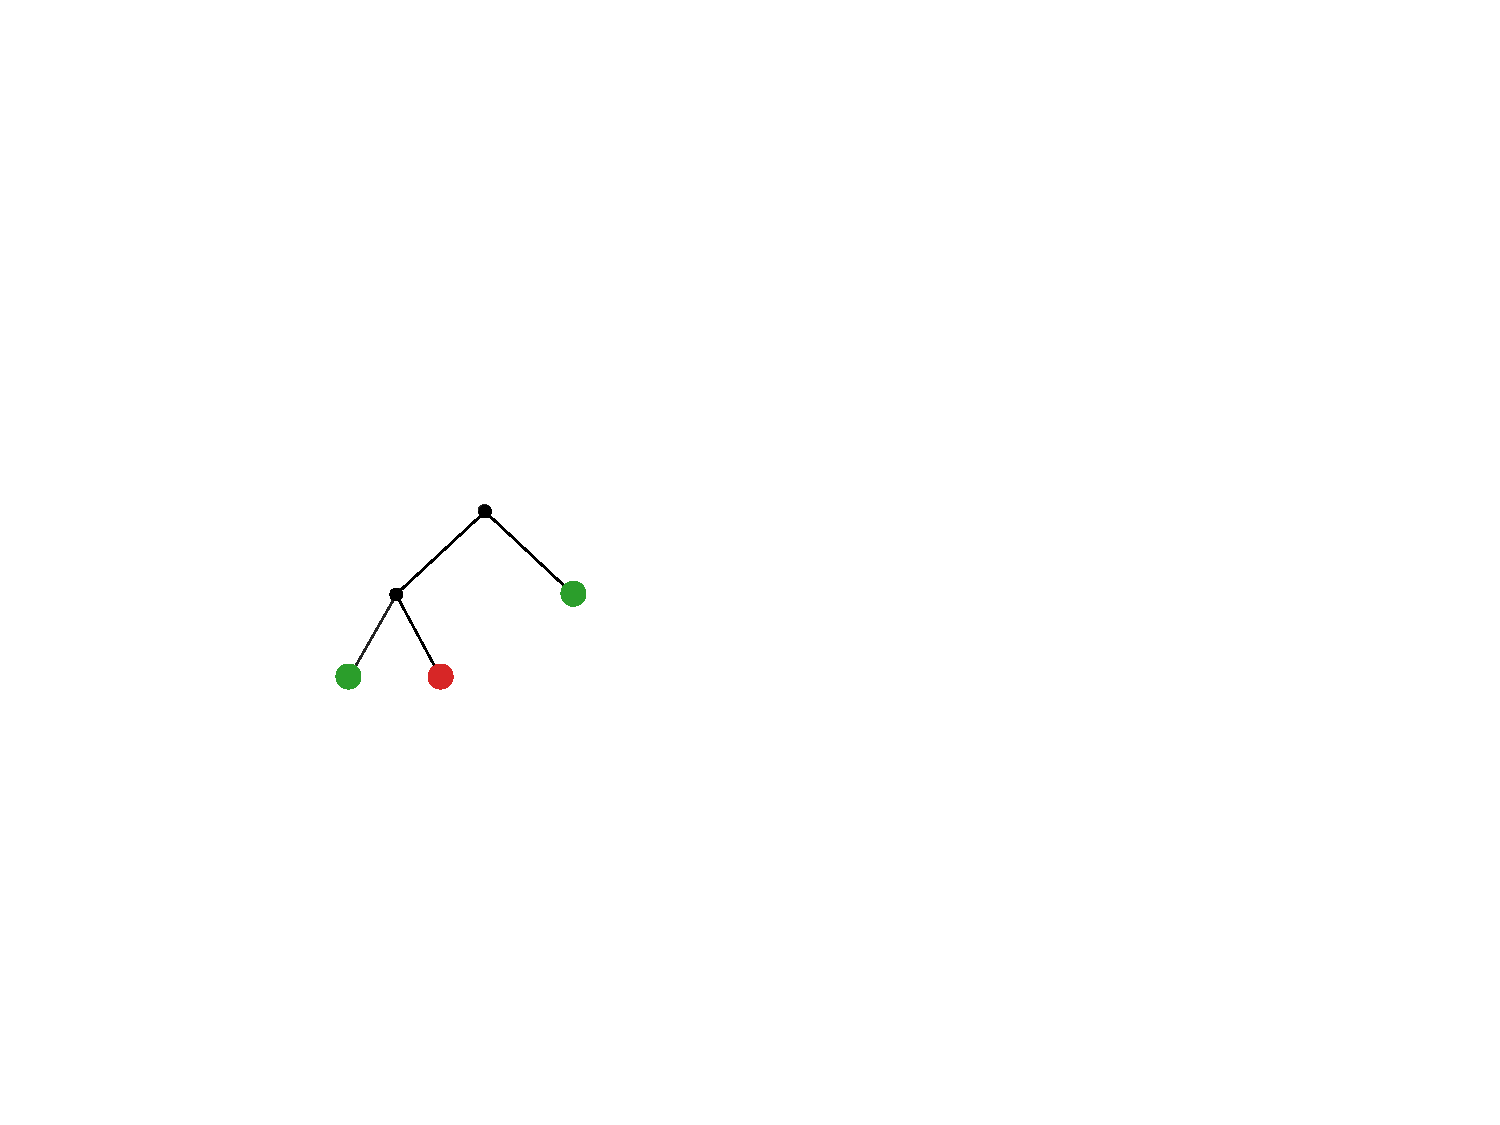
\includegraphics[width=\ratio\linewidth, trim={100 150 430 200}, clip]{ser_0.pdf}
%         \onslide<2>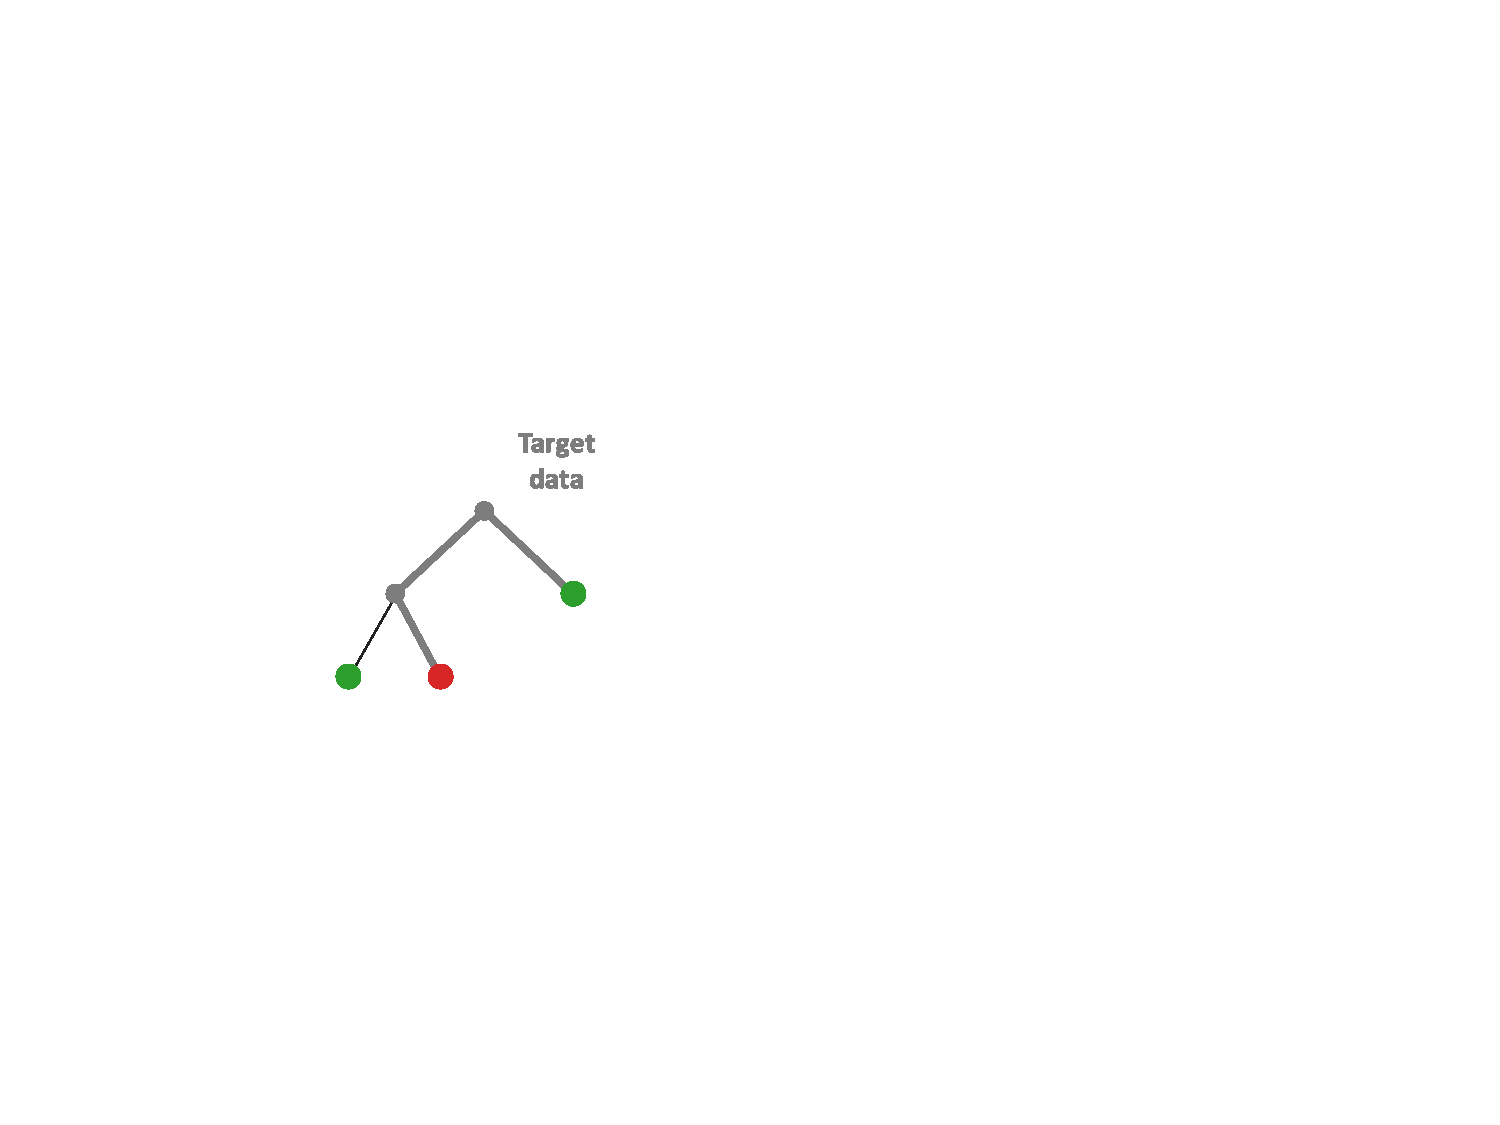
\includegraphics[width=\ratio\linewidth, trim={100 150 430 200}, clip]{ser_1.pdf}
%         \onslide<3>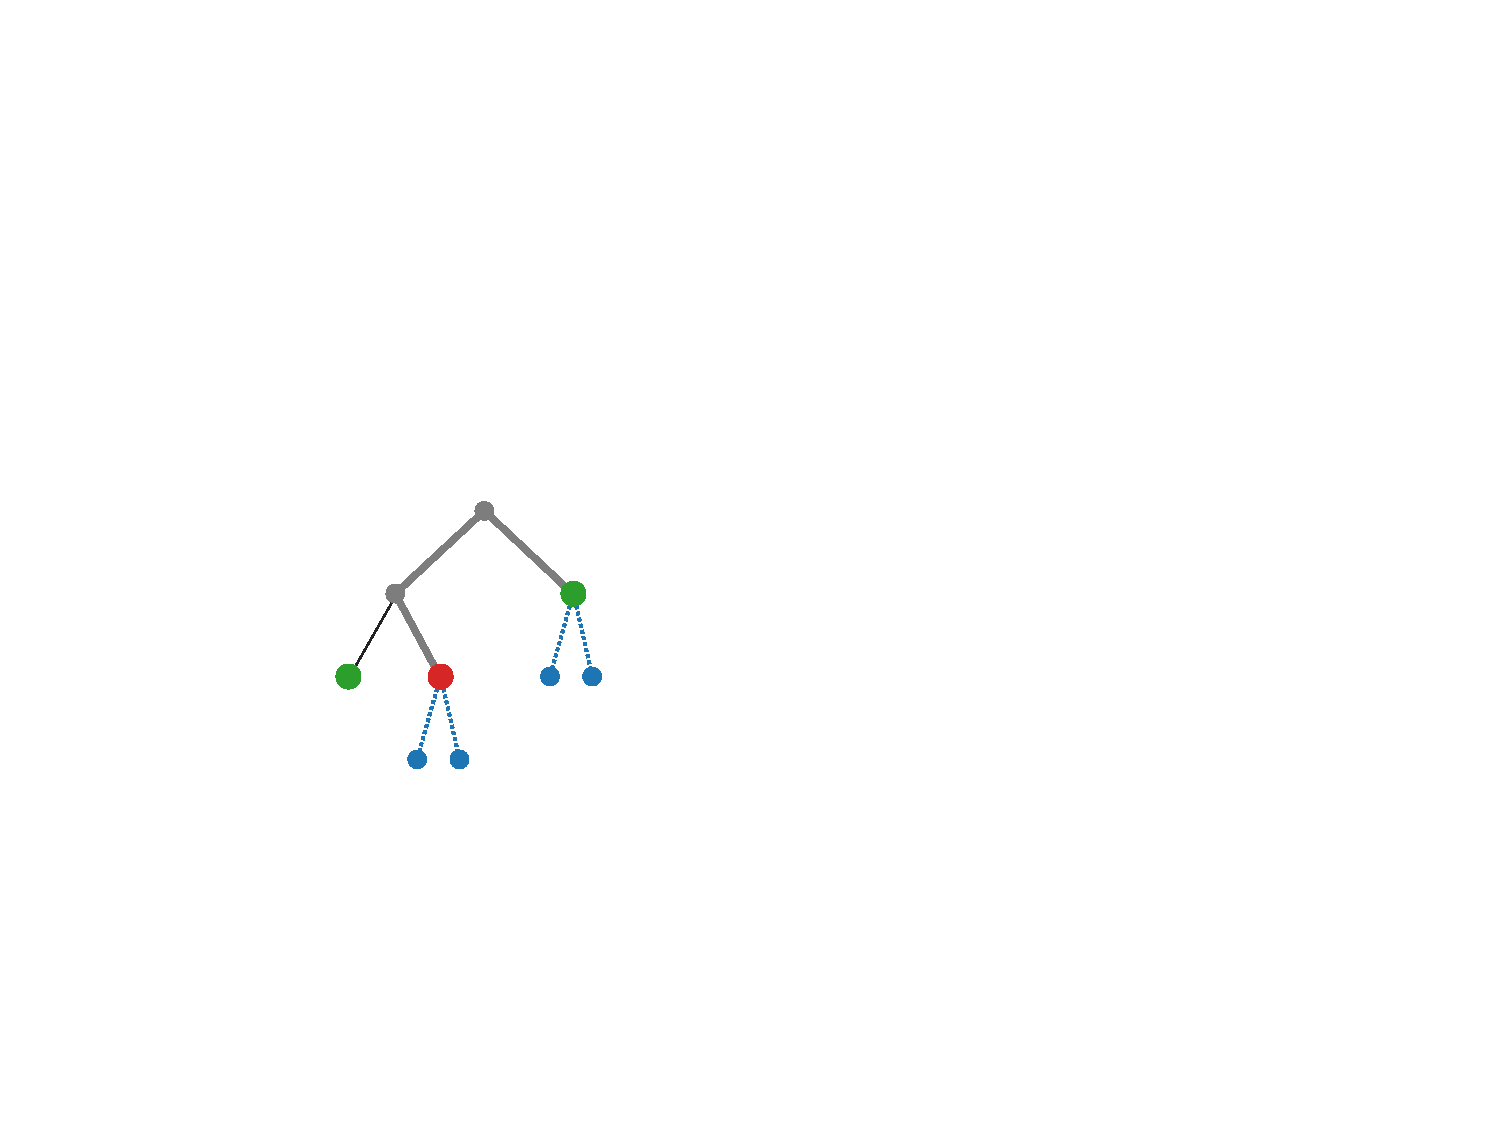
\includegraphics[width=\ratio\linewidth, trim={100 150 430 200}, clip]{ser_2.pdf}
%         \onslide<4>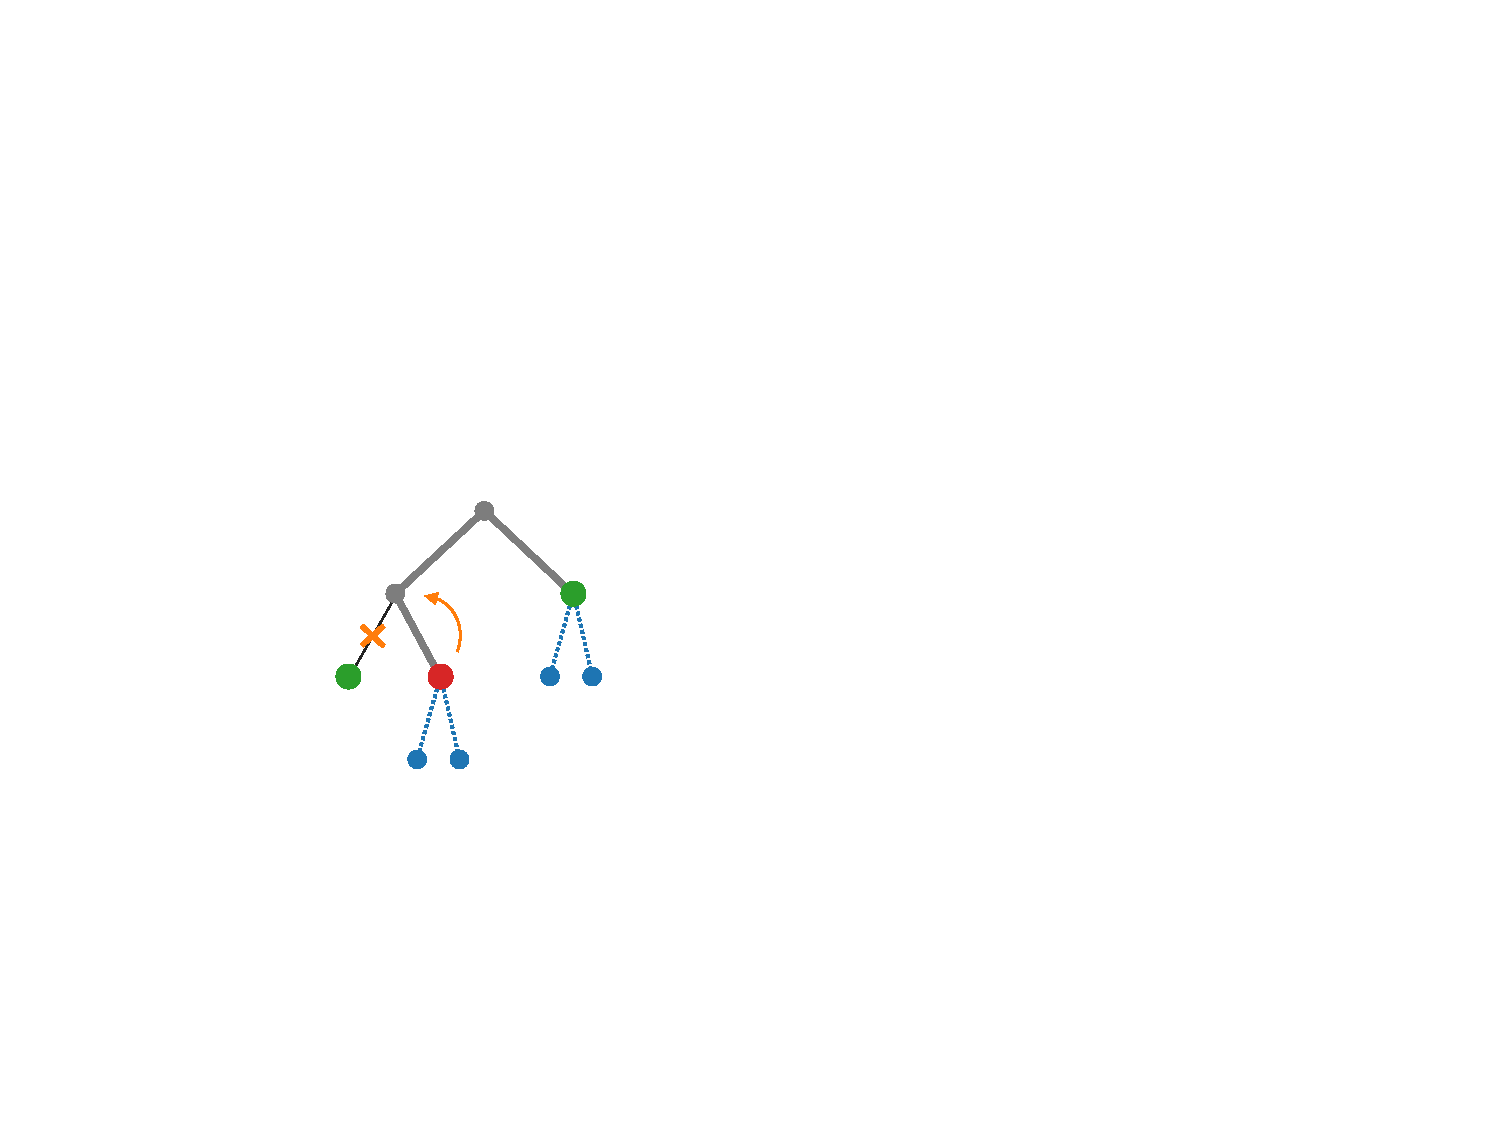
\includegraphics[width=\ratio\linewidth, trim={100 150 430 200}, clip]{ser_3.pdf}
%         \onslide<5->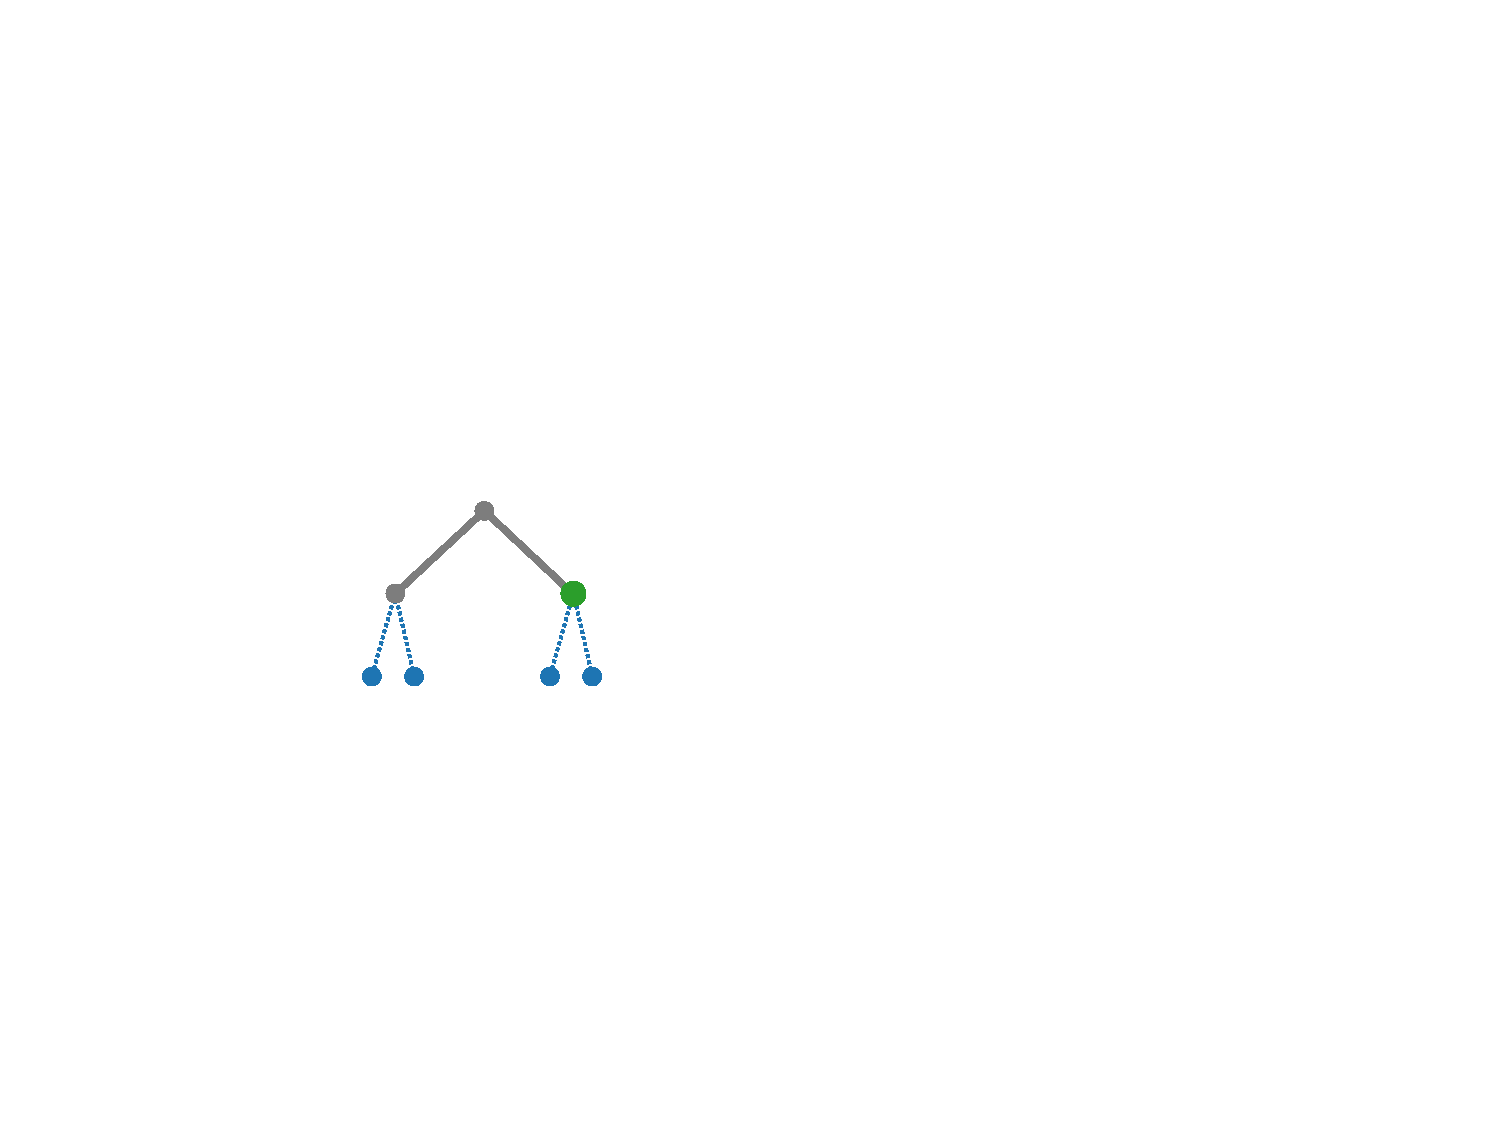
\includegraphics[width=\ratio\linewidth, trim={100 150 430 200}, clip]{ser_4.pdf}
%     \end{overprint}
    \begin{overprint}
        \onslide<1>\centering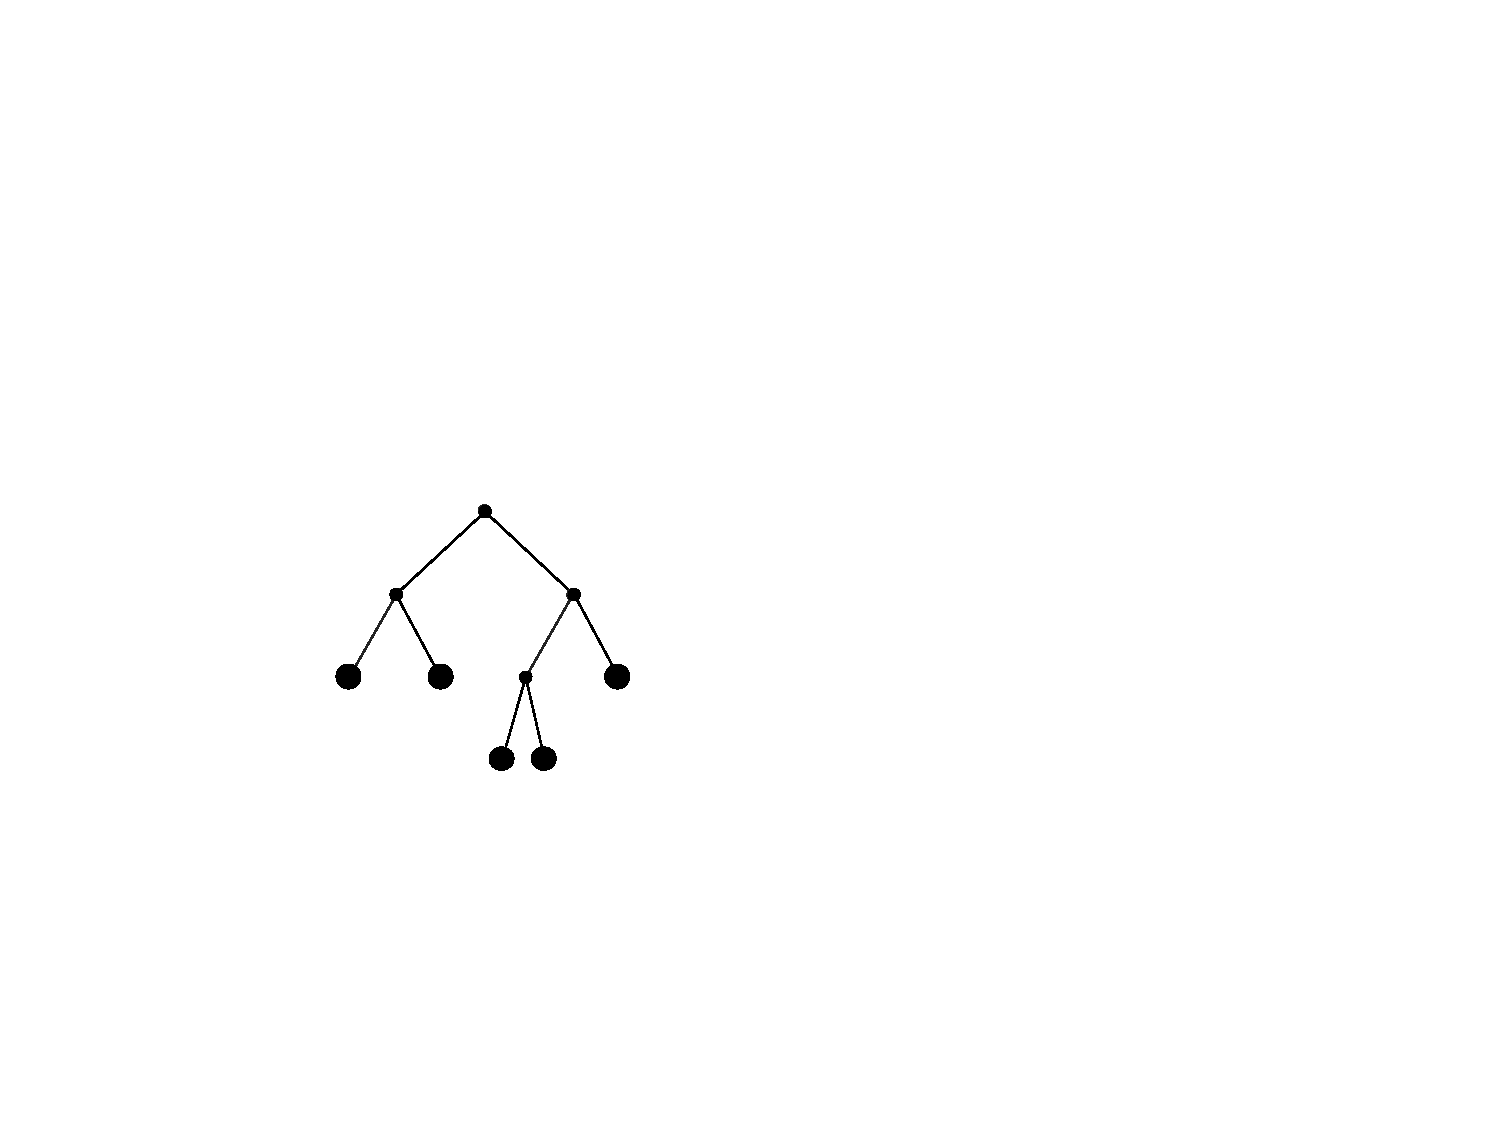
\includegraphics[width=\ratio\linewidth, trim={150 120 410 200}, clip]{schemas_ser_1.pdf}
        \onslide<2>\centering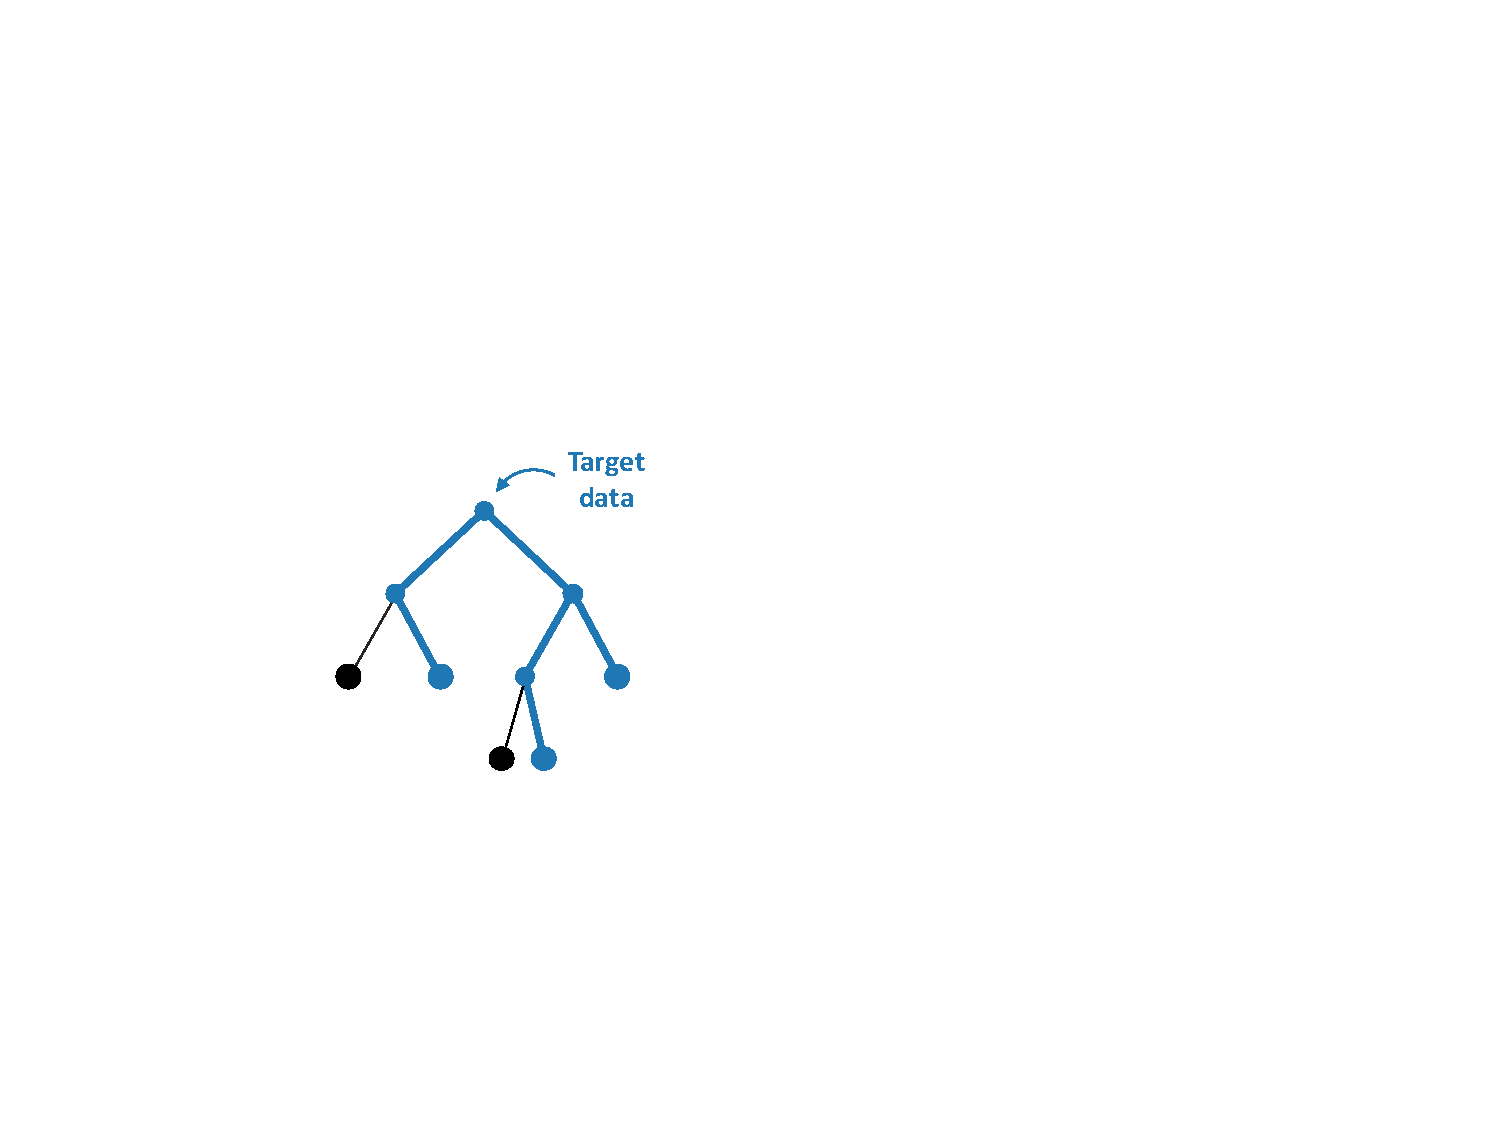
\includegraphics[width=\ratio\linewidth, trim={150 120 410 200}, clip]{schemas_ser_2.pdf}
        \onslide<3>\centering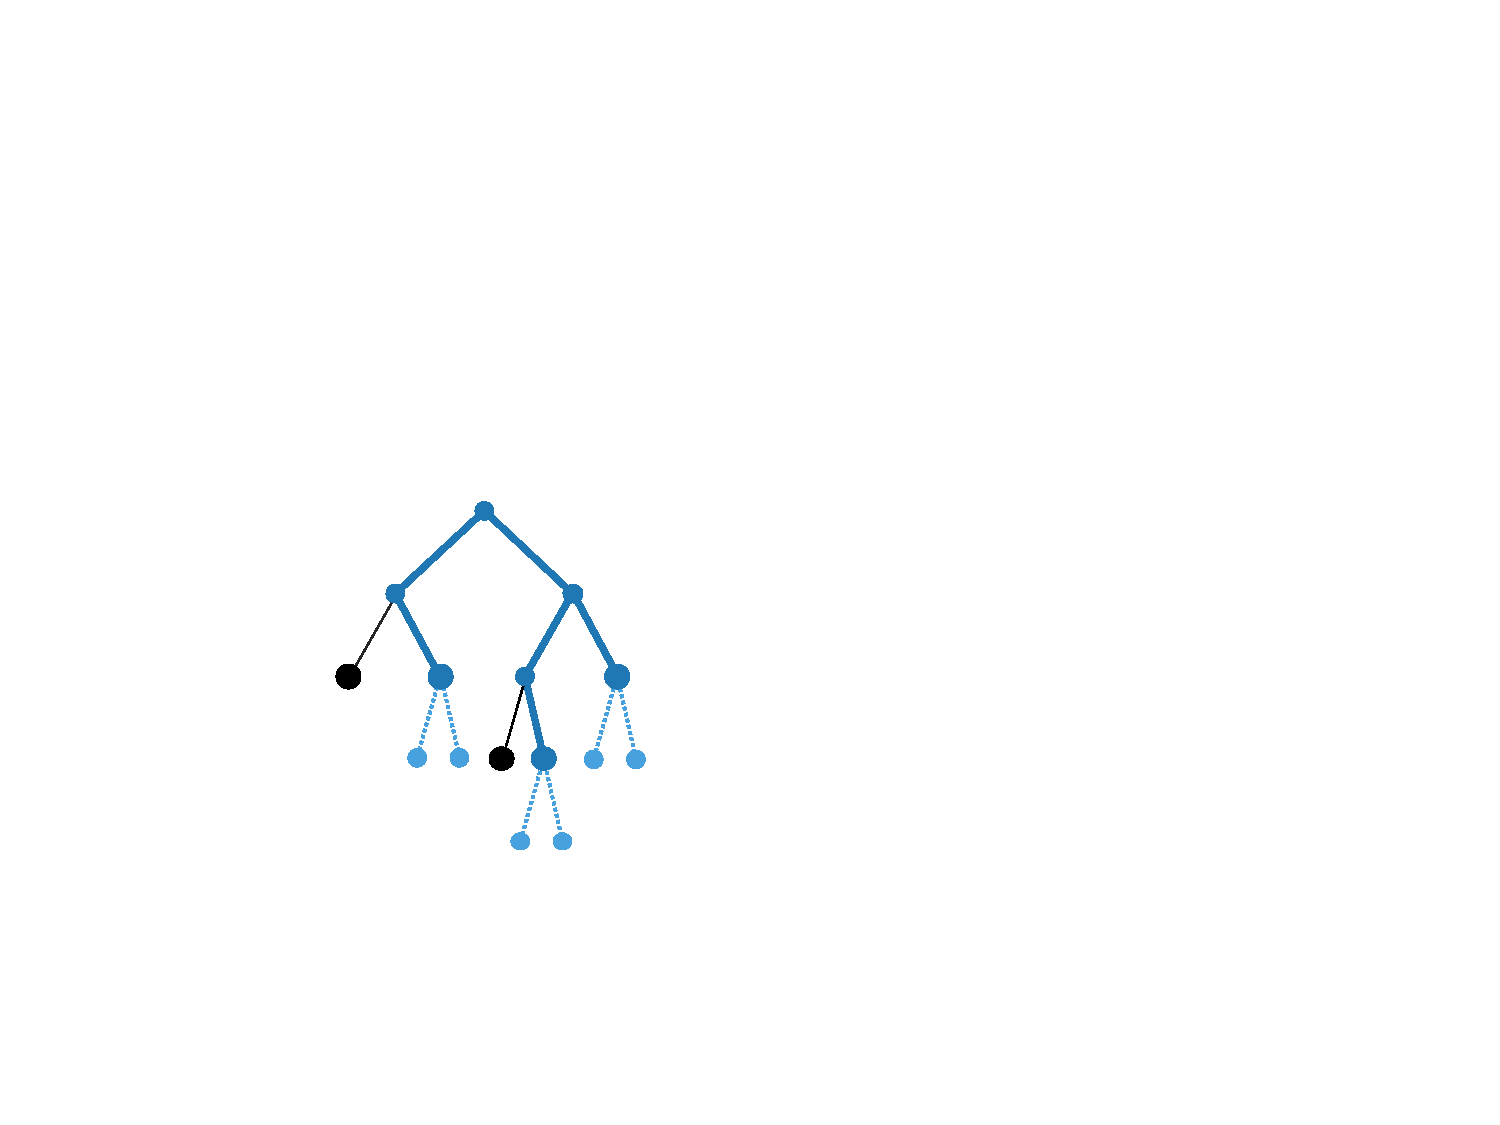
\includegraphics[width=\ratio\linewidth, trim={150 120 410 200}, clip]{schemas_ser_3.pdf}
        \onslide<4>\centering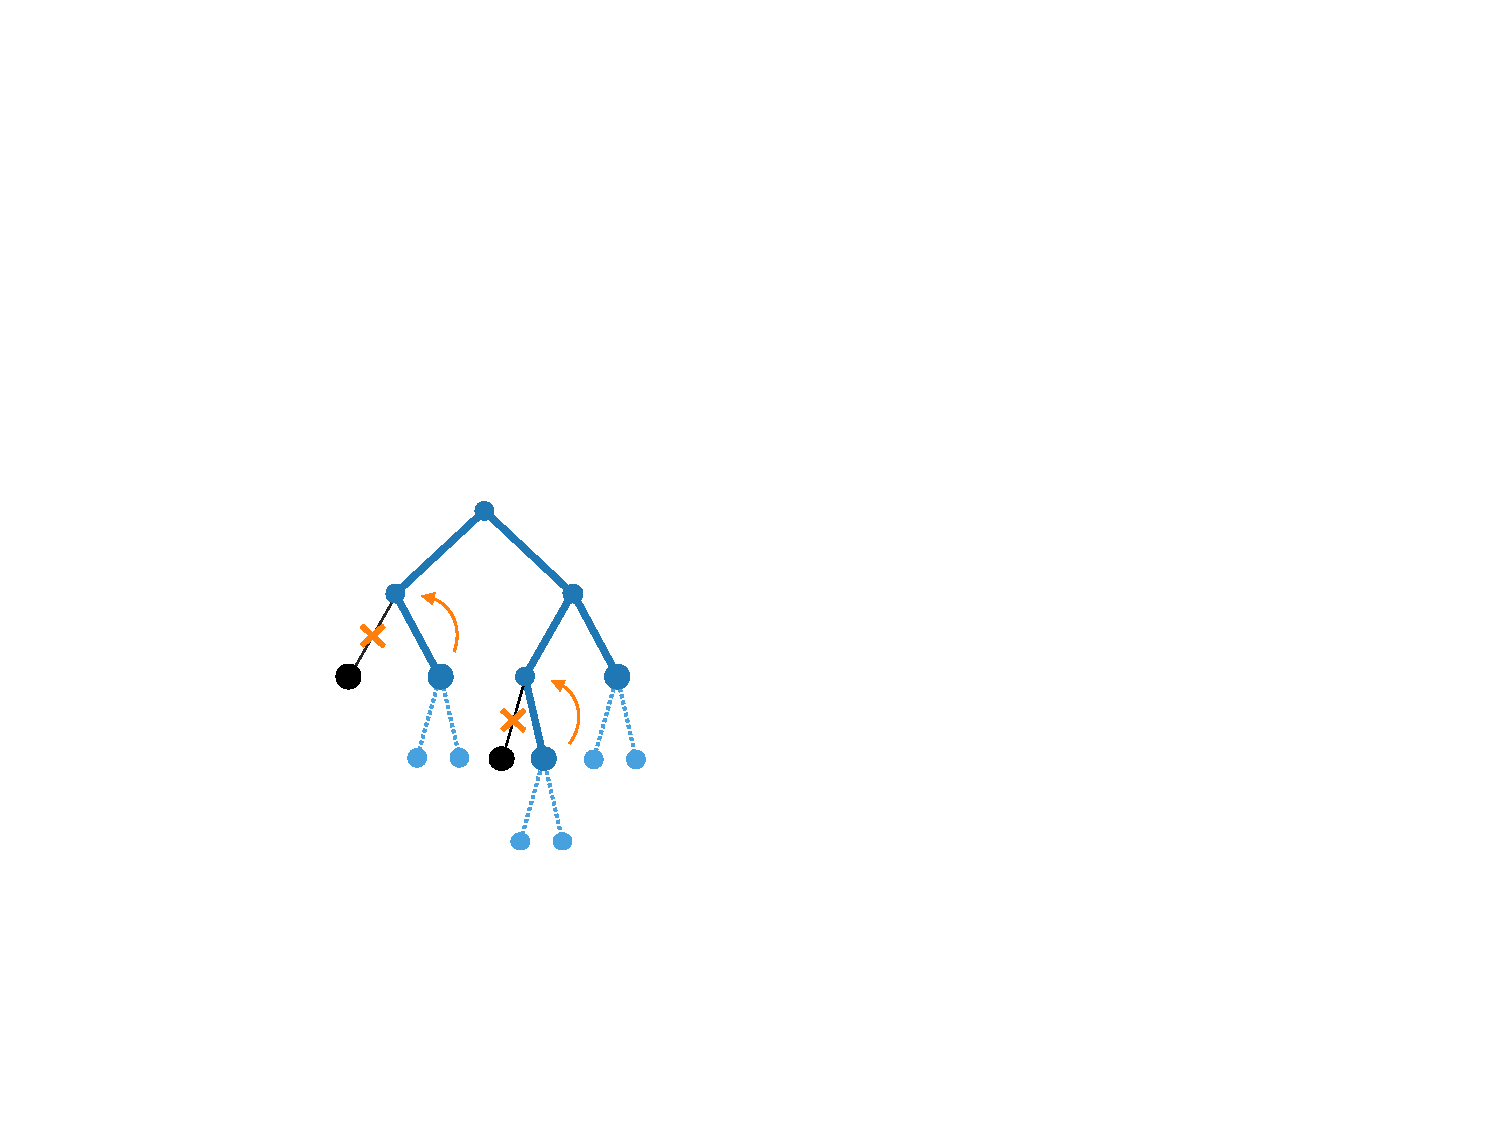
\includegraphics[width=\ratio\linewidth, trim={150 120 410 200}, clip]{schemas_ser_4.pdf}
        \onslide<5->\centering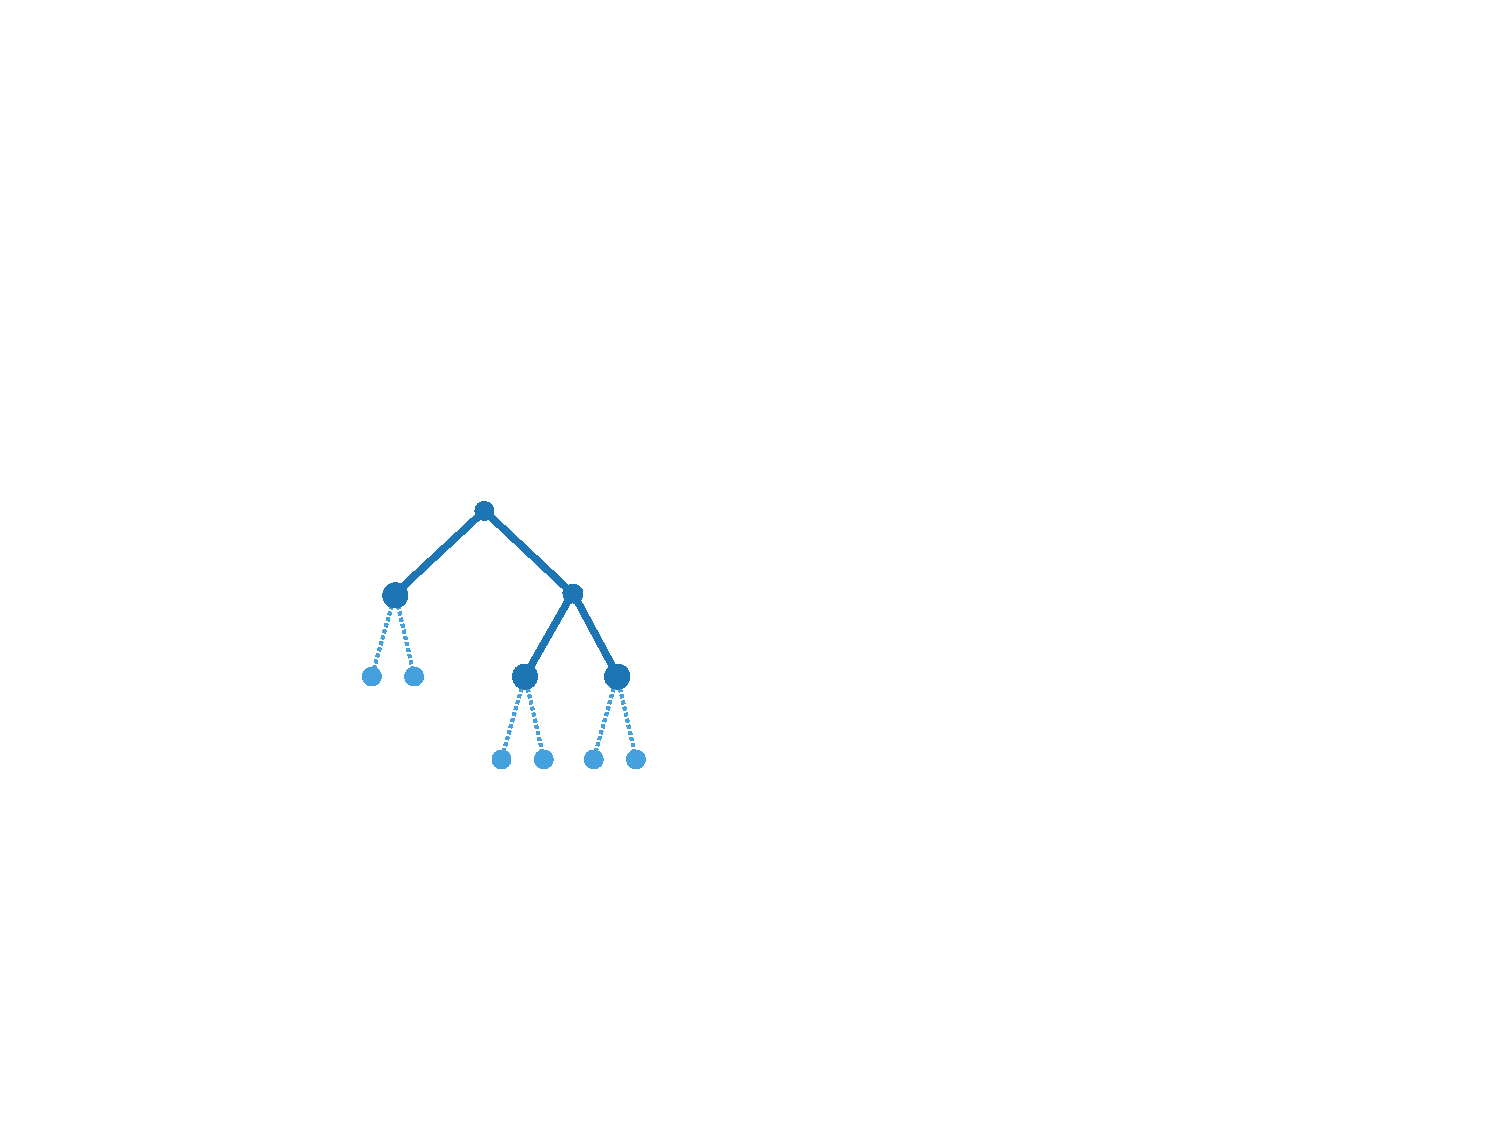
\includegraphics[width=\ratio\linewidth, trim={150 120 410 200}, clip]{schemas_ser_5.pdf}
    \end{overprint}
    
    \pause \pause
    \textcolor{myblue}{1. Expansion}\\
    \pause
    \textcolor{myorange}{2. Reduction}\\
    \smallskip
    \onslide<11->{Partition refinement or simplification}

\end{minipage}\hfill
\begin{minipage}[t]{0.49\linewidth}
    \vspace{0pt}
    \centering
    \pause \pause
    \textbf{Structure Transfer (STRUT)}
    
    \renewcommand{\ratio}{0.55}
%     \begin{overprint}
%         \onslide<6>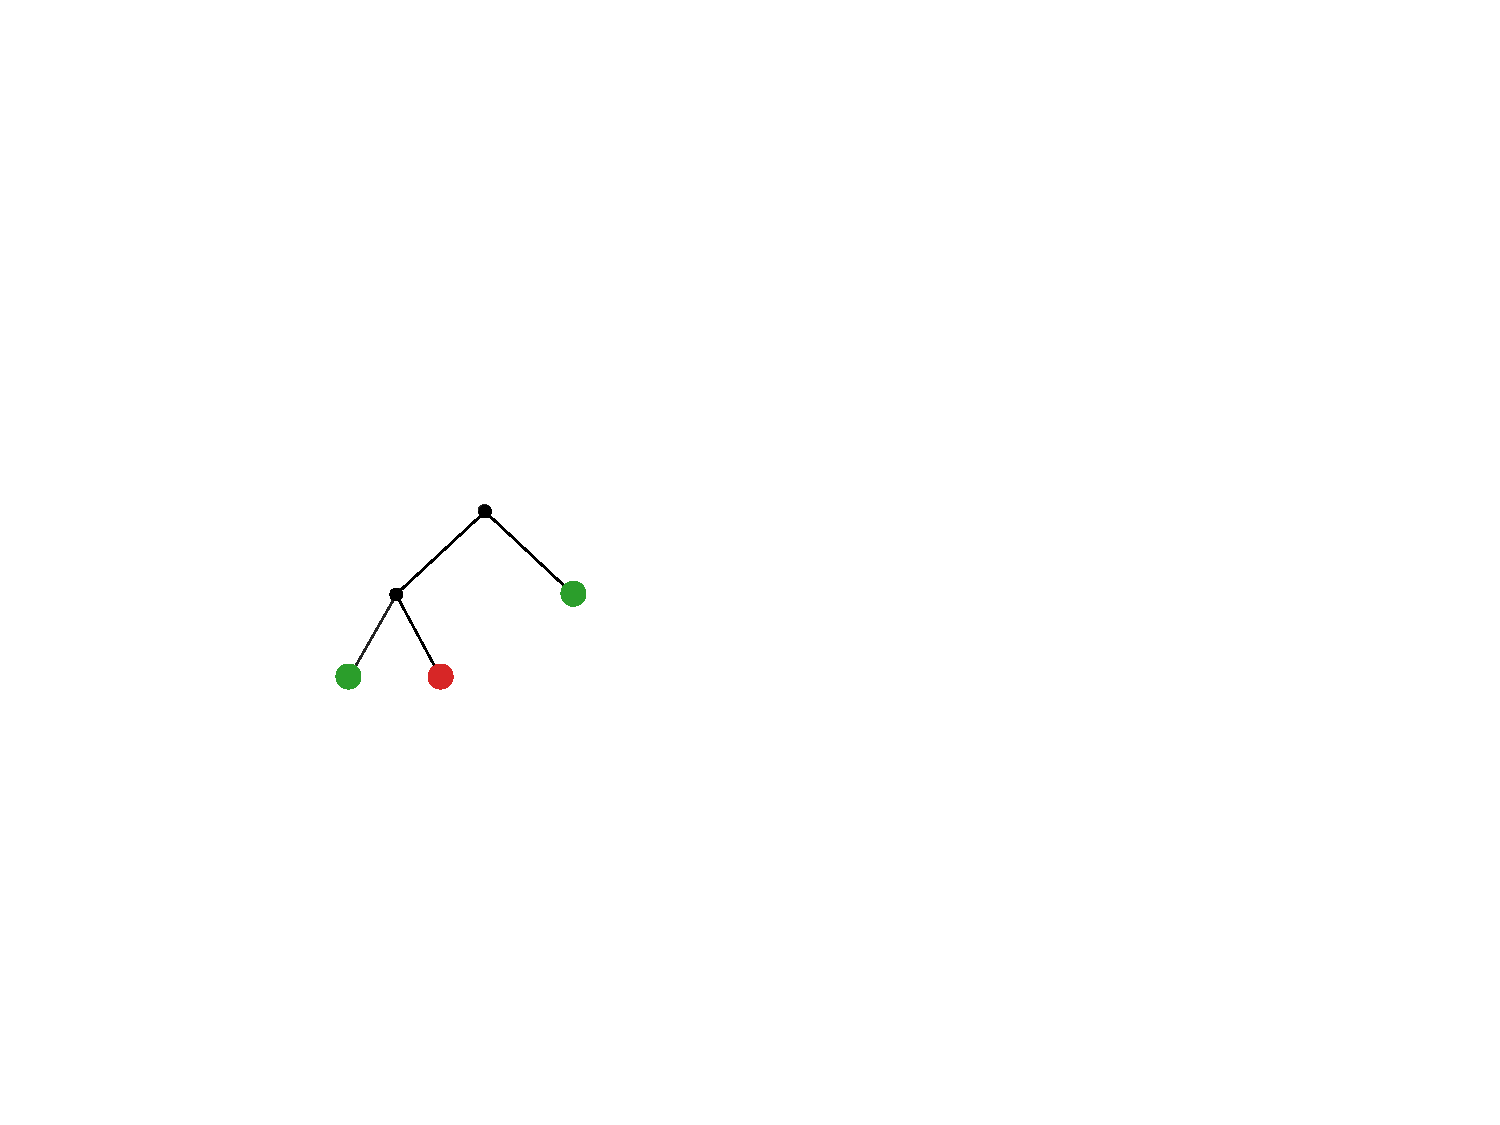
\includegraphics[width=\ratio\linewidth, trim={100 180 430 200}, clip]{strut_0.pdf}
%         \onslide<7>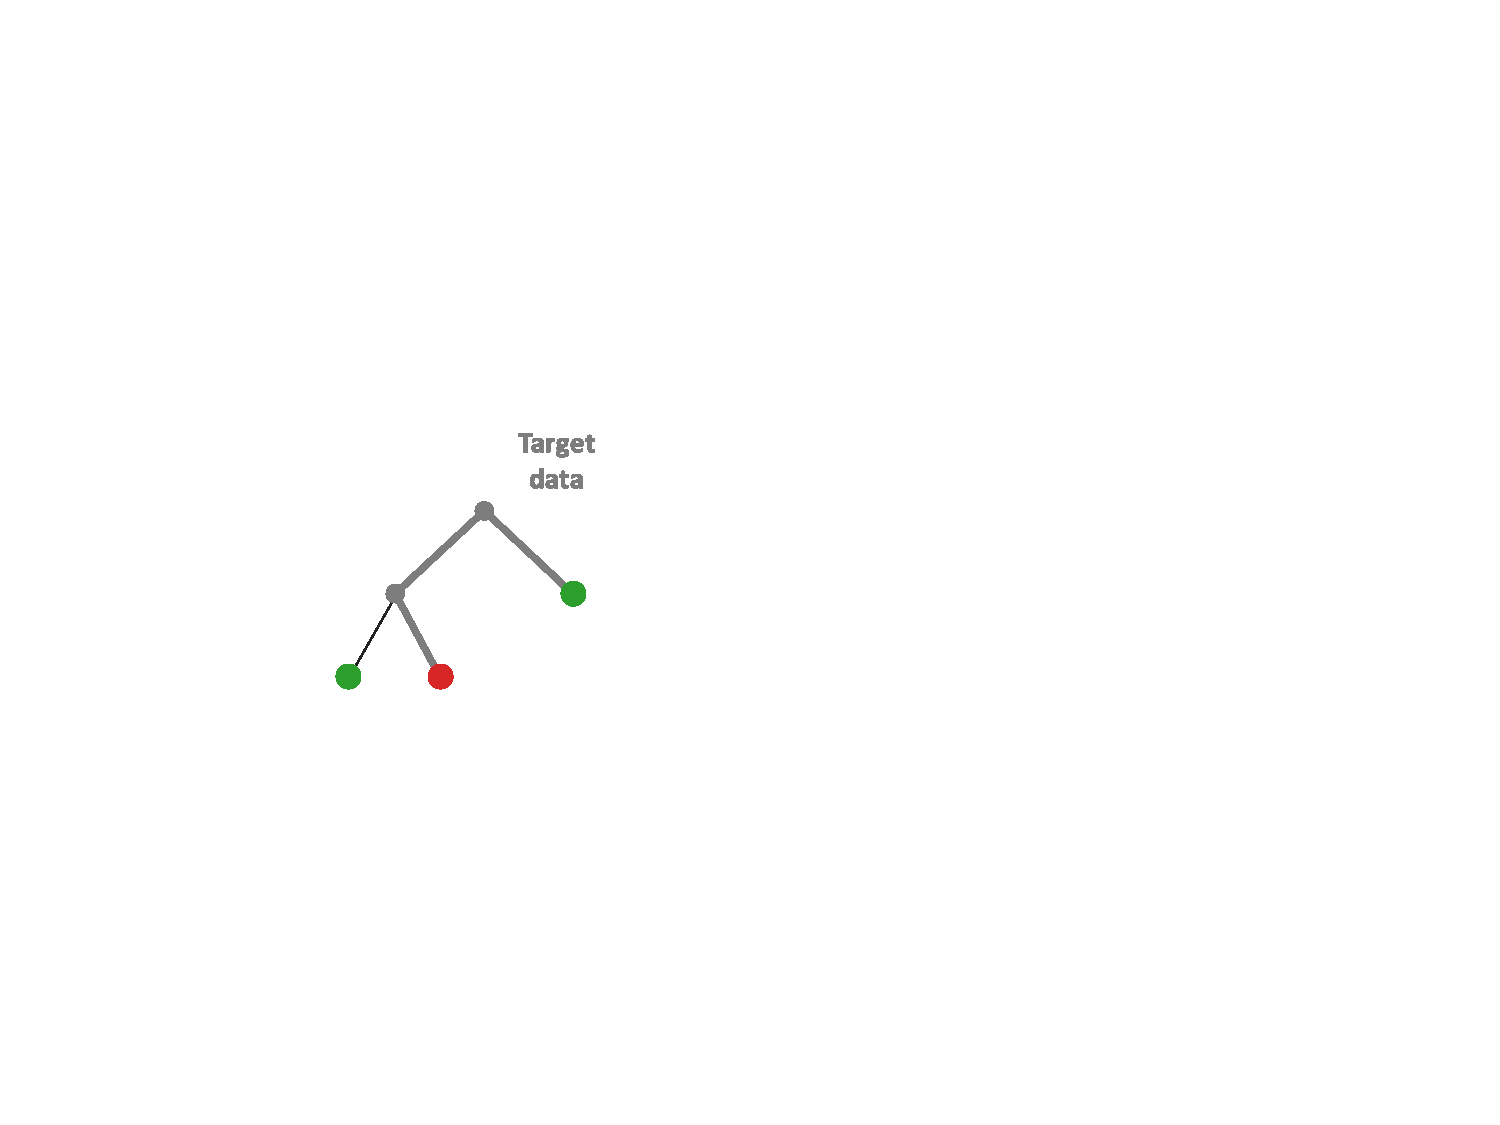
\includegraphics[width=\ratio\linewidth, trim={100 180 430 200}, clip]{strut_1.pdf}
%         \onslide<8>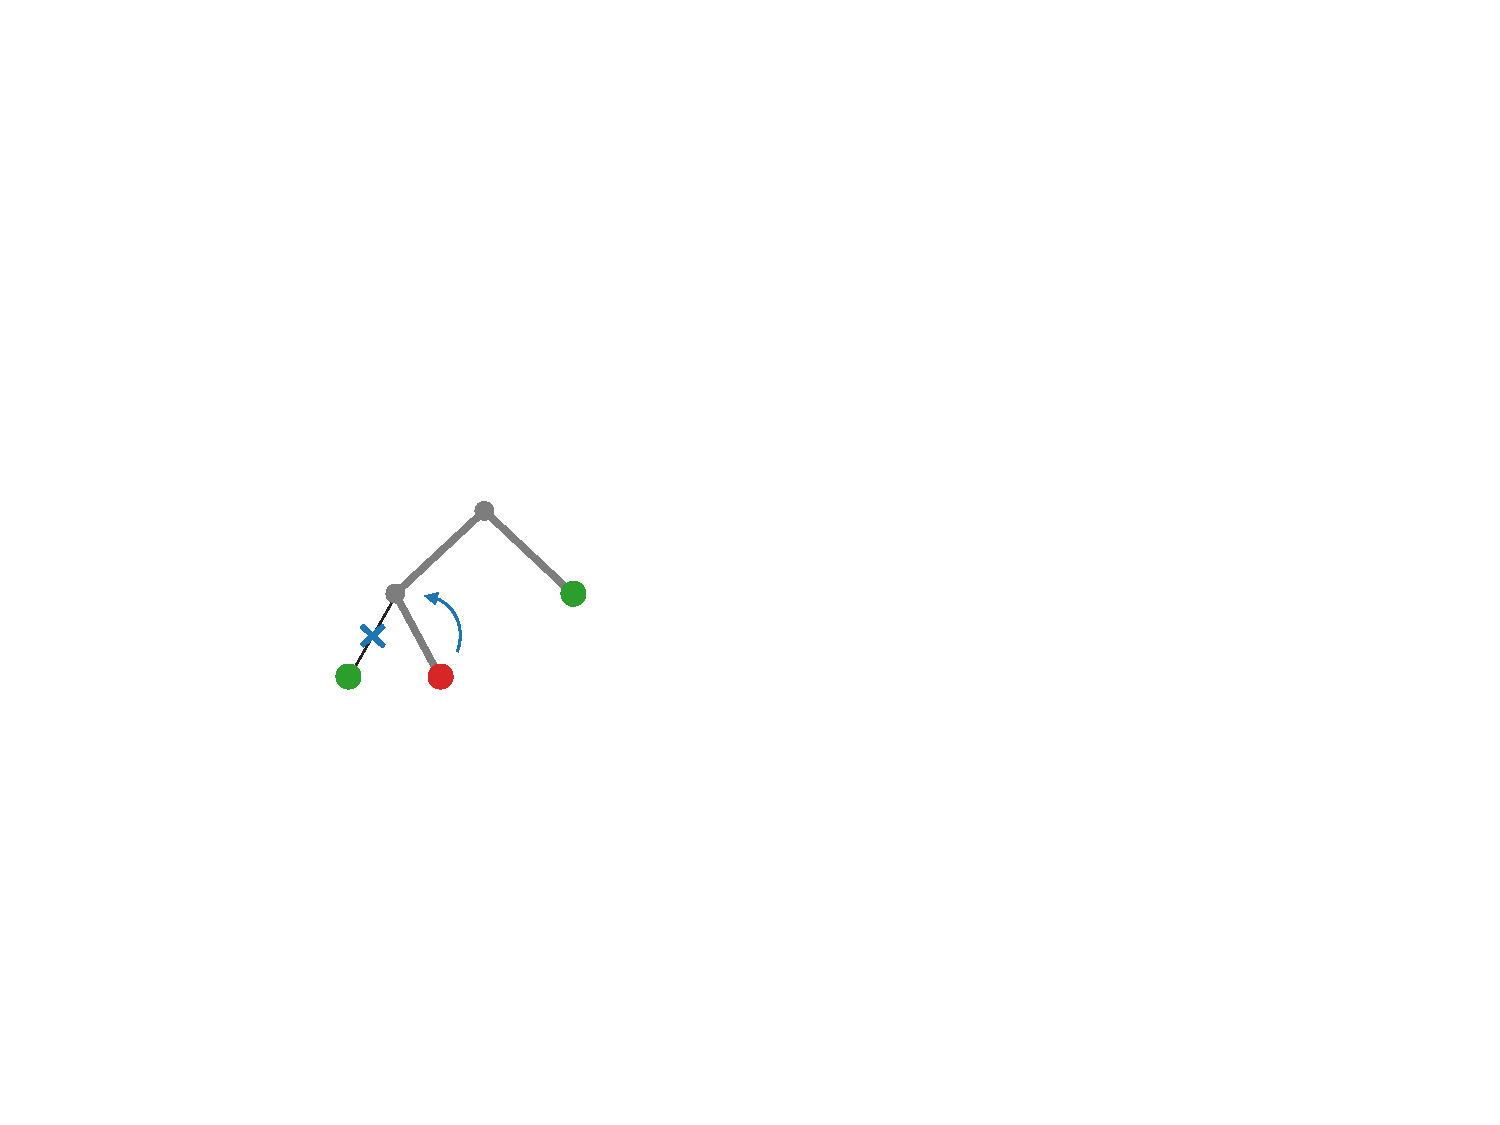
\includegraphics[width=\ratio\linewidth, trim={100 180 430 200}, clip]{strut_2.pdf}
%         \onslide<9>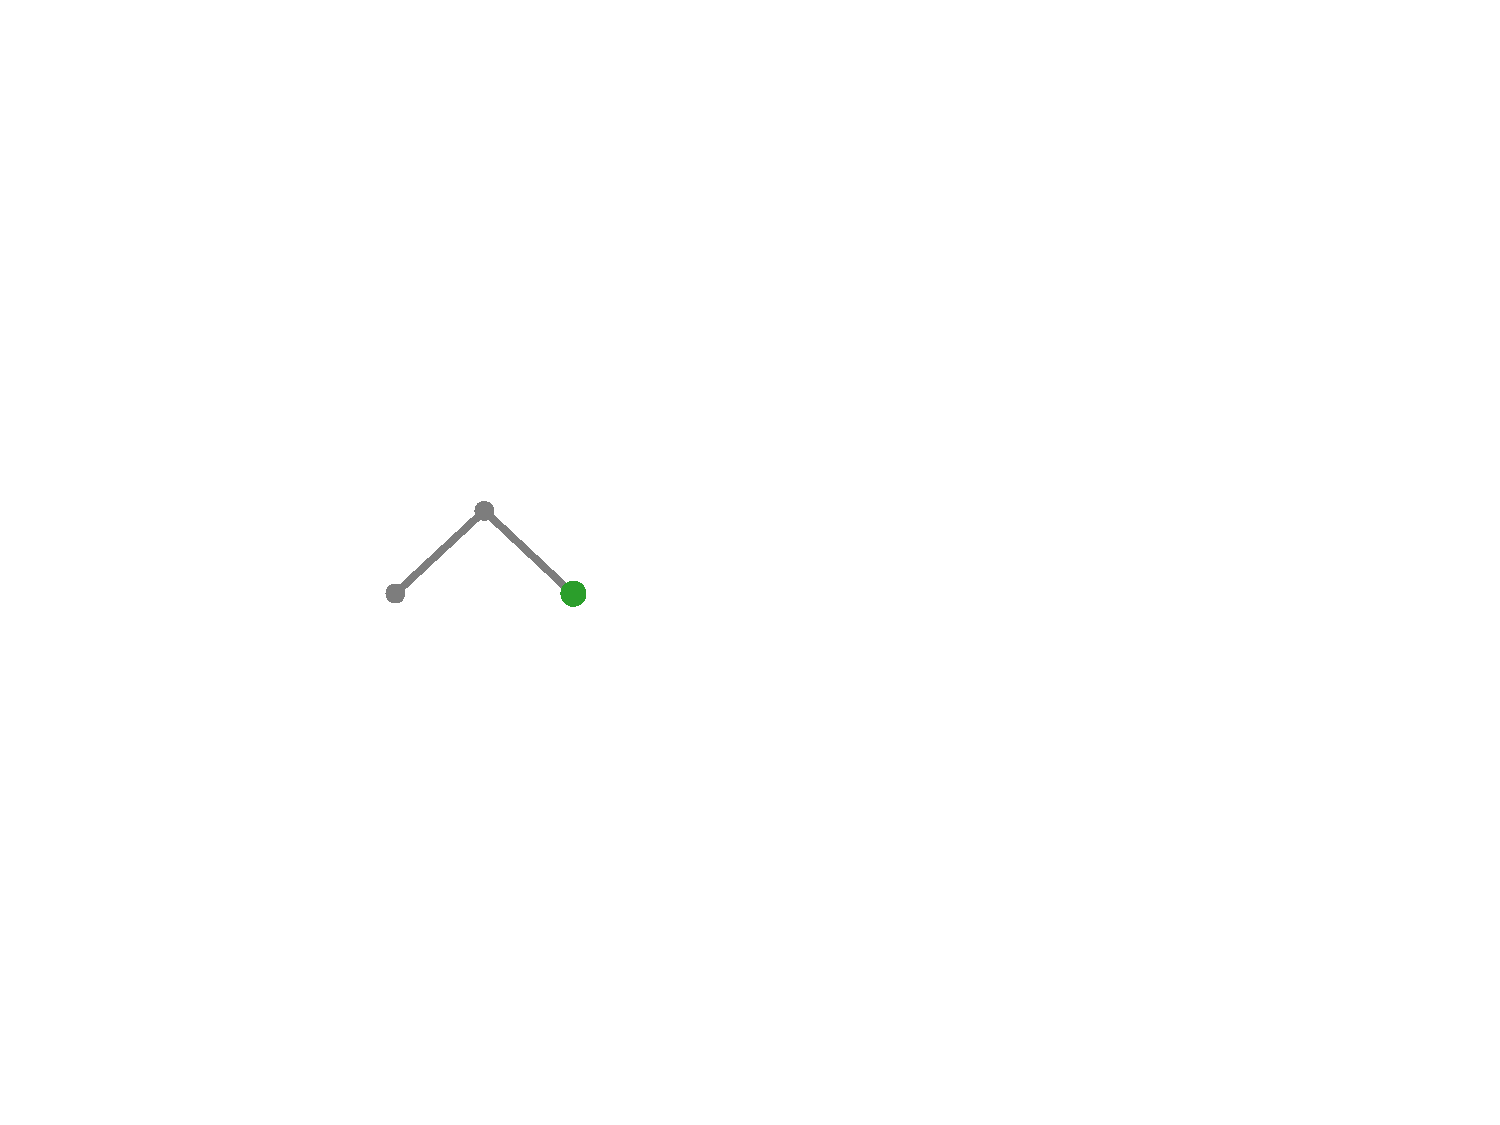
\includegraphics[width=\ratio\linewidth, trim={100 180 430 200}, clip]{strut_3.pdf}
%         \onslide<10->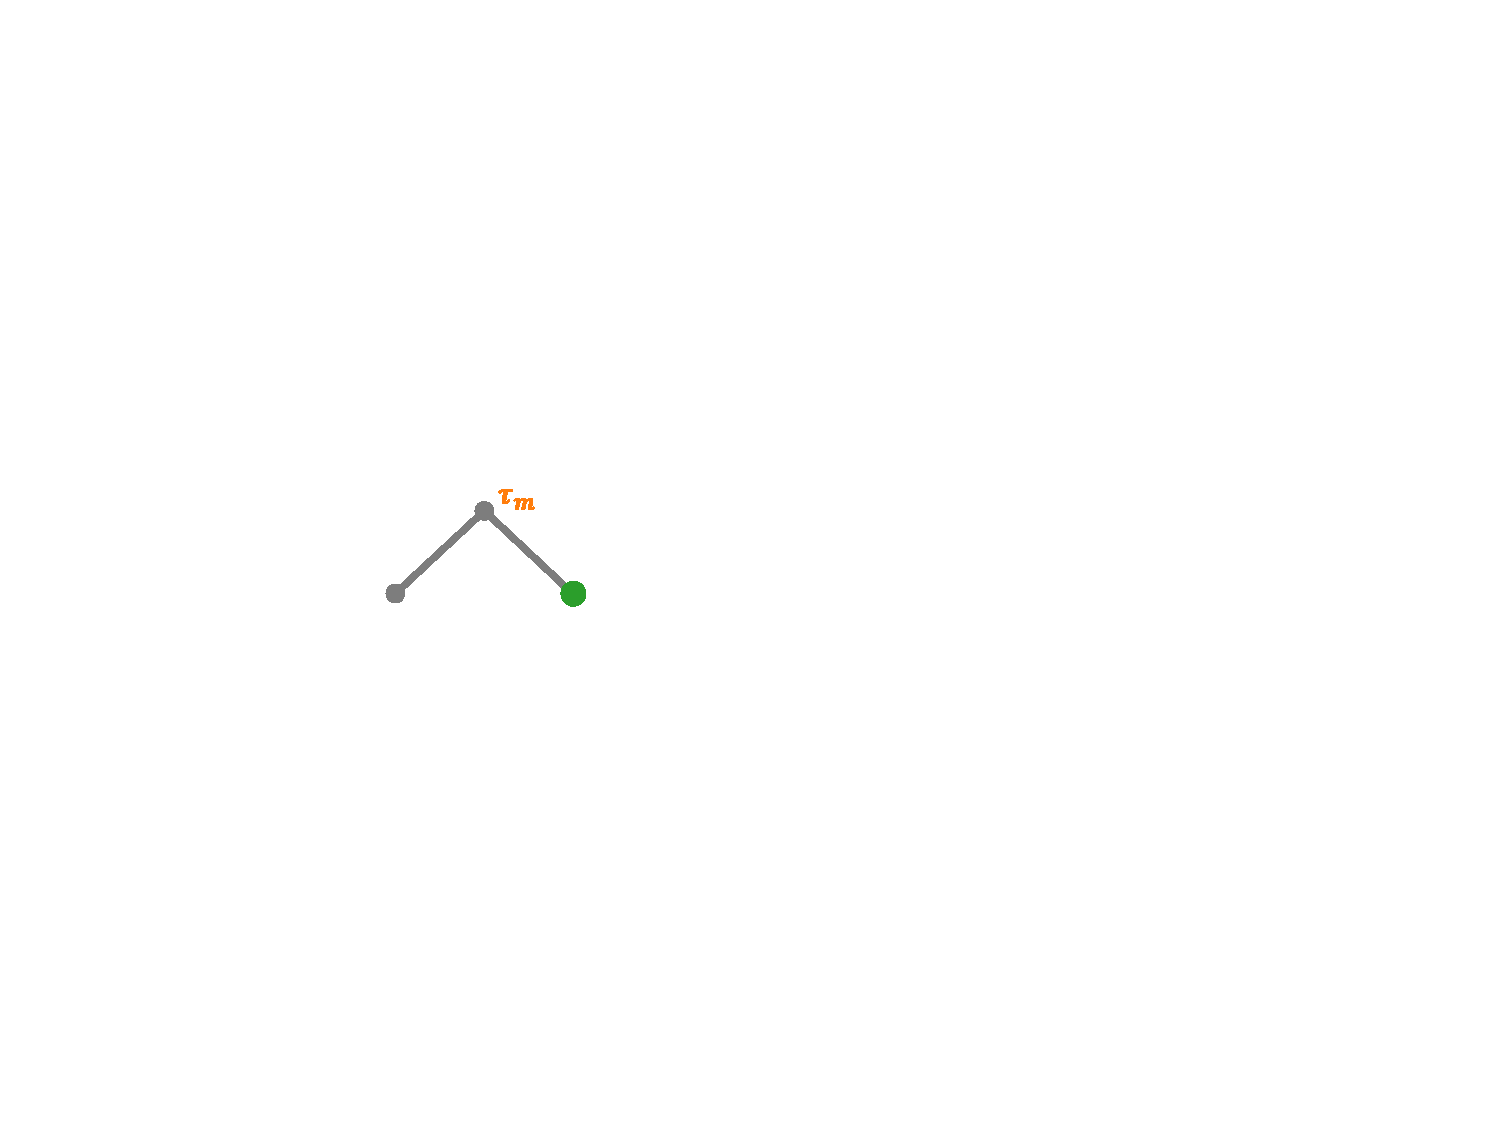
\includegraphics[width=\ratio\linewidth, trim={100 180 430 200}, clip]{strut_4.pdf}
%     \end{overprint}
    \begin{overprint}
        \onslide<6>\centering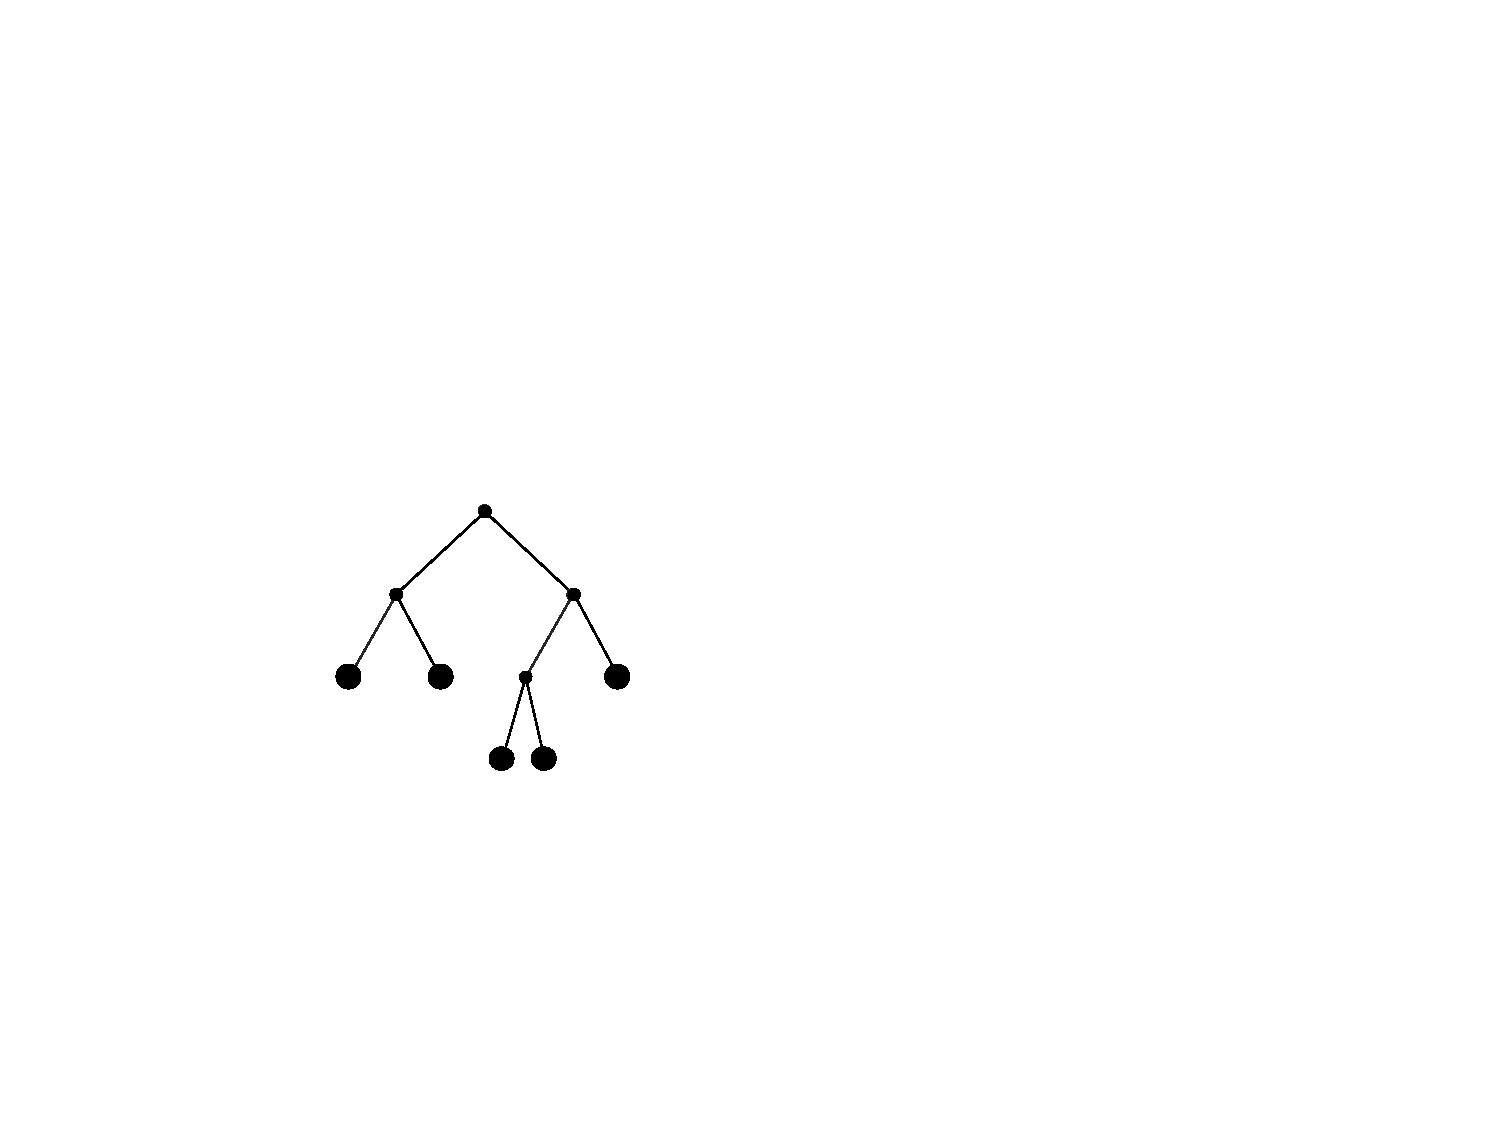
\includegraphics[width=\ratio\linewidth, trim={140 150 410 200}, clip]{schemas_strut_1_15.pdf}
        \onslide<7>\centering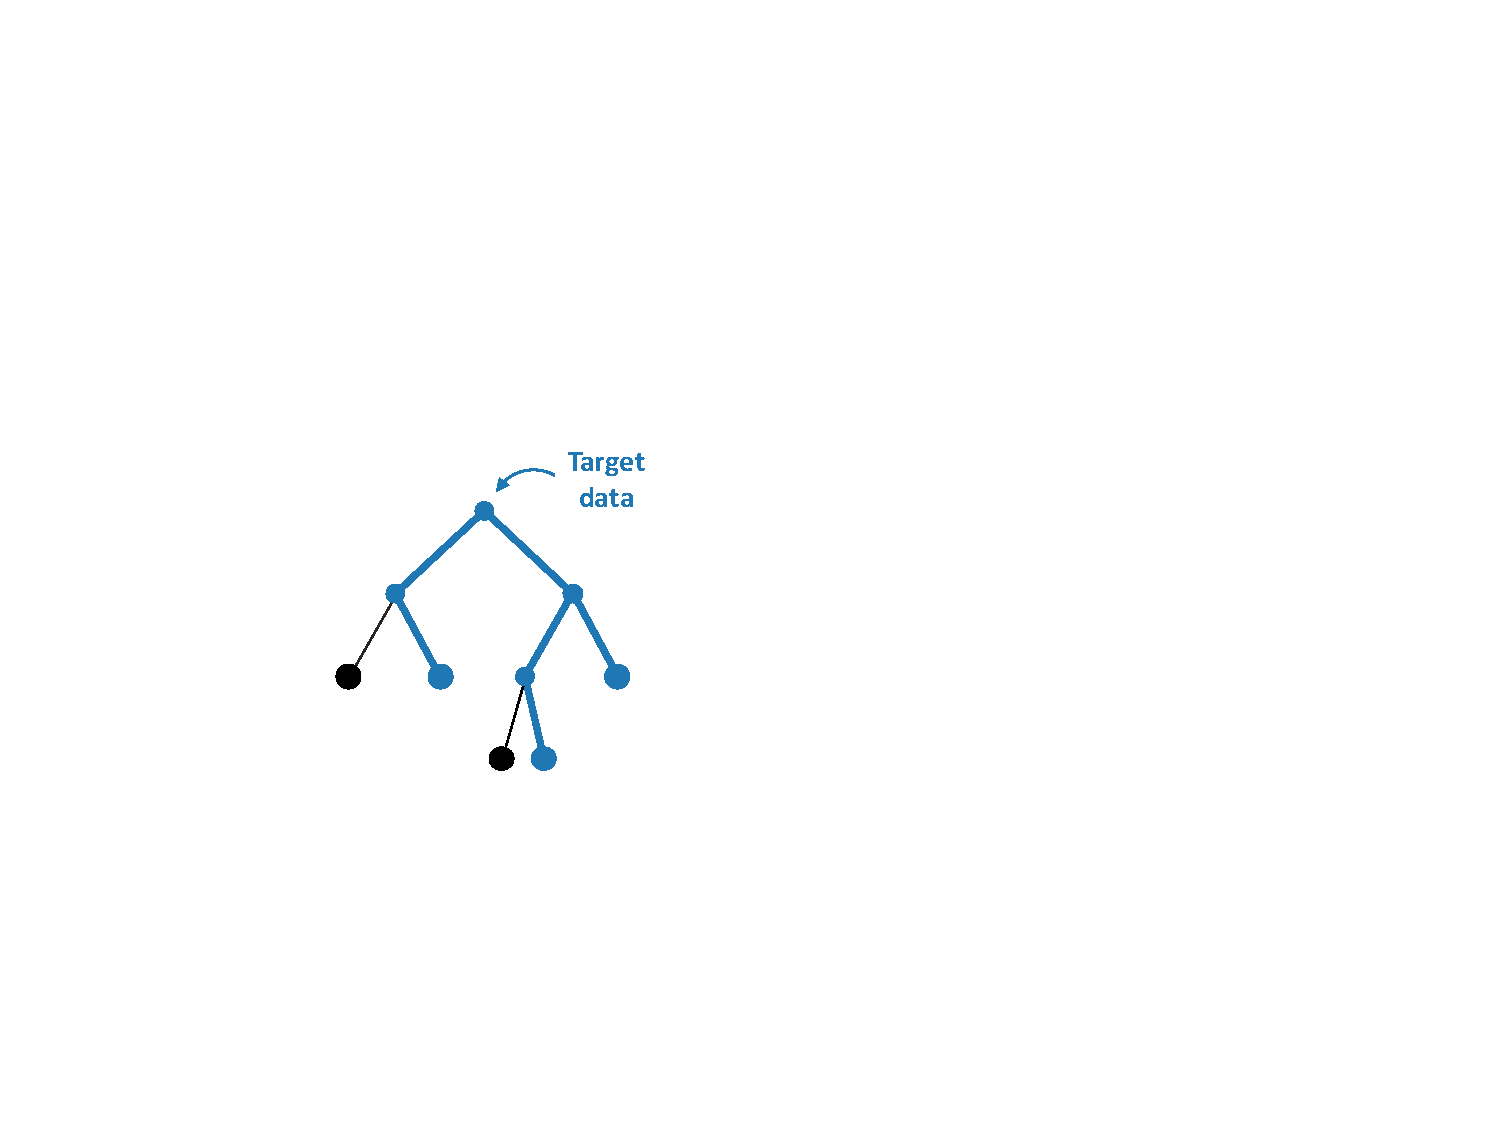
\includegraphics[width=\ratio\linewidth, trim={140 150 410 200}, clip]{schemas_strut_2_15.pdf}
        \onslide<8>\centering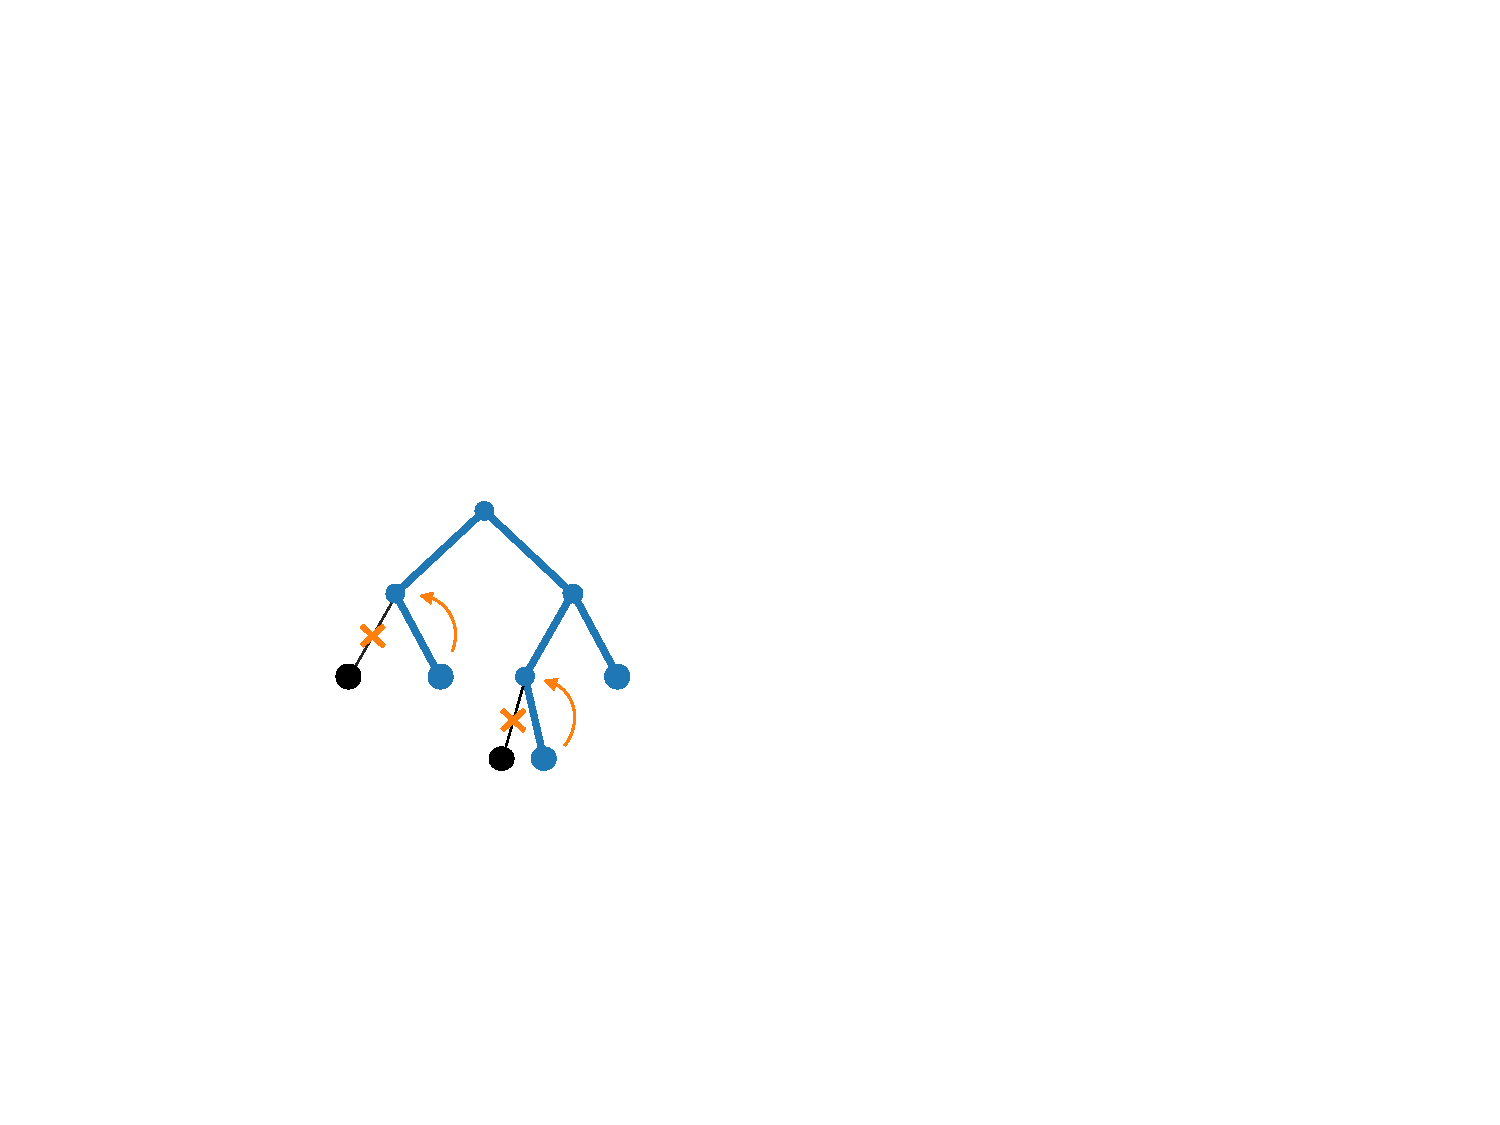
\includegraphics[width=\ratio\linewidth, trim={140 150 410 200}, clip]{schemas_strut_3_15.pdf}
        \onslide<9>\centering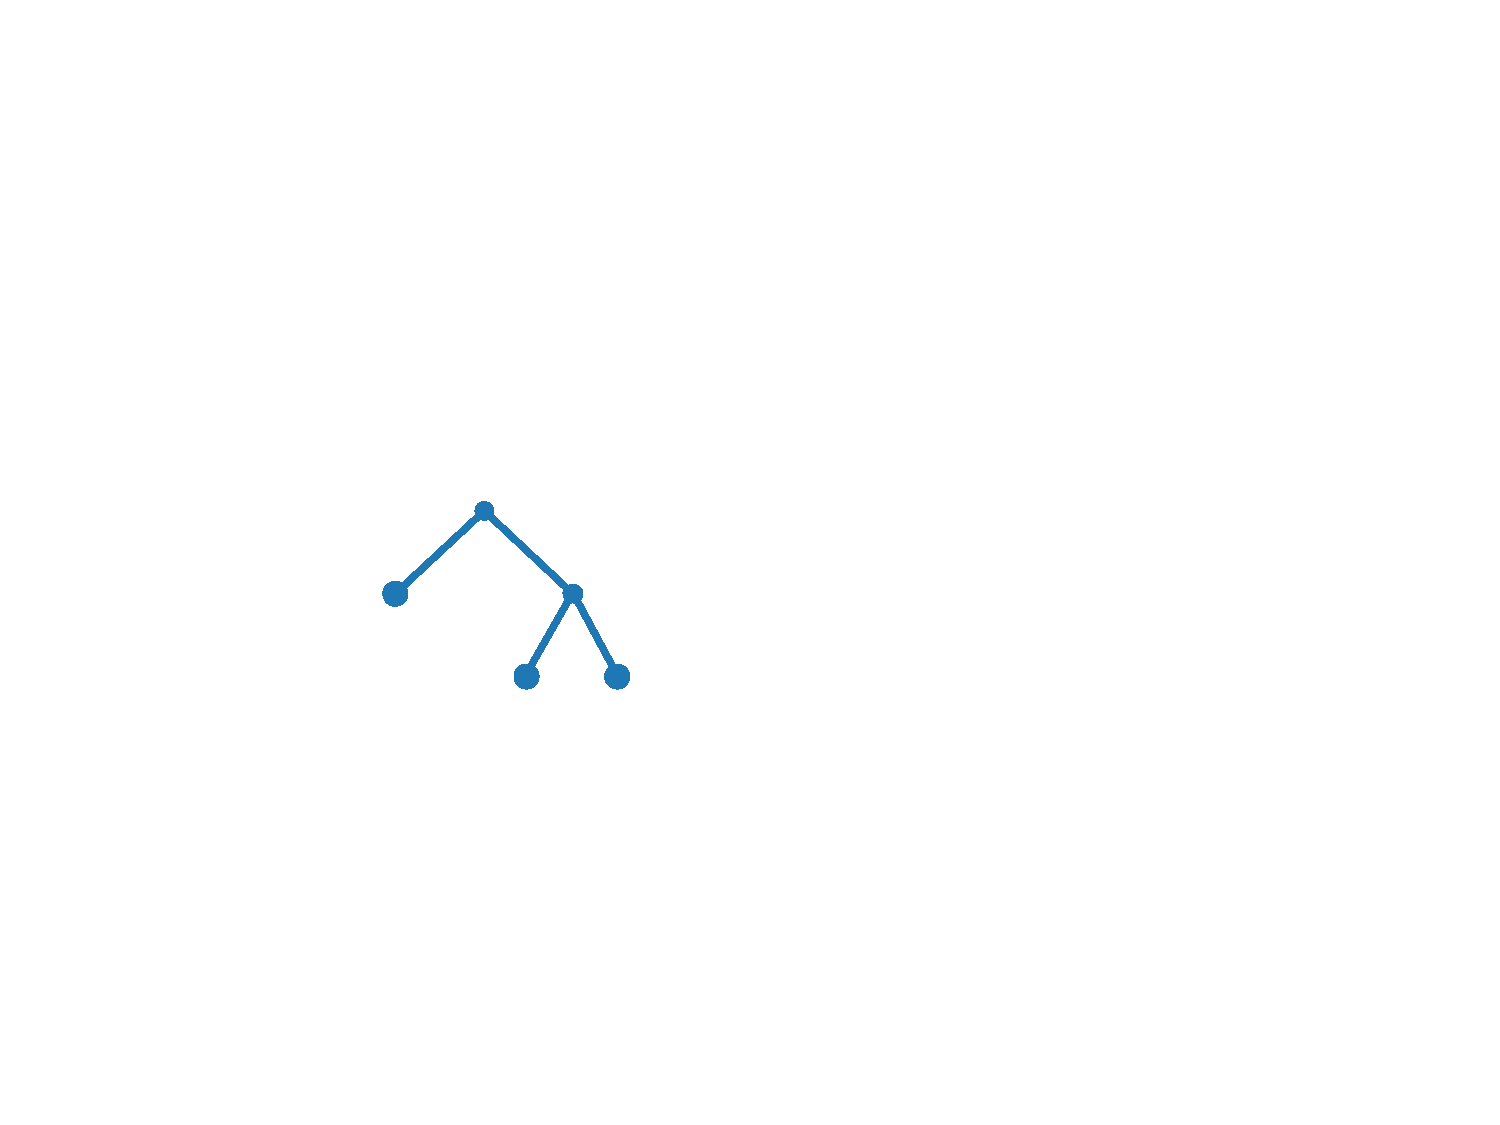
\includegraphics[width=\ratio\linewidth, trim={140 150 410 200}, clip]{schemas_strut_4_15.pdf}
        \onslide<10->\centering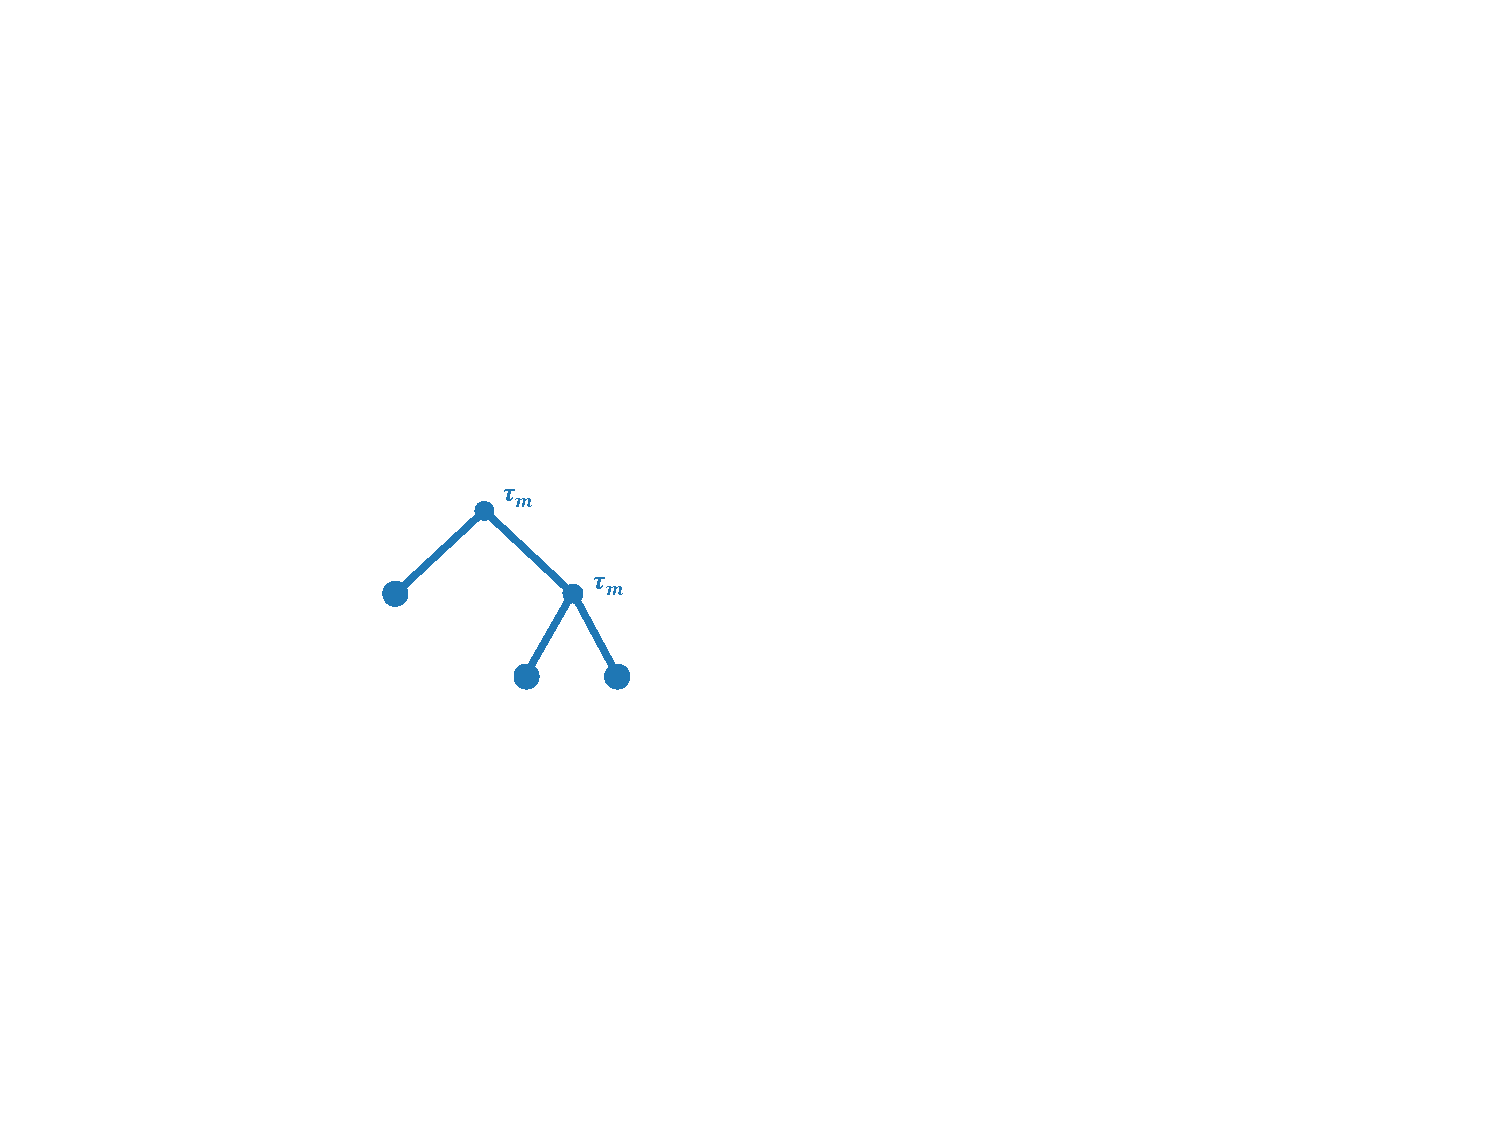
\includegraphics[width=\ratio\linewidth, trim={140 150 410 200}, clip]{schemas_strut_5_15.pdf}
    \end{overprint}
    \onslide<8->
    \textcolor{myorange}{1. Pruning}\\
    \onslide<10->
    \textcolor{myblue}{2. Threshold update}\\
    \smallskip
    \onslide<11->
    Drifts
\end{minipage}

\centering
\medskip
\pause[12]
\textcolor{myblue}{How about imbalanced data ?}

\end{frame}

\subsection{Leaf loss risk}

\begin{frame}{Leaf loss risk}

\begin{minipage}[t]{0.38\textwidth}
    \vspace{0pt}
    \begin{tcolorbox}[title=Homogeneous class imbalance,size=title,boxrule=0.2pt]
    \begin{align*}
        & P^T(x|y) = P^S(x|y) \\
        & P^T(y|x) = \lambda_y \frac{P^S(y|x)}{\int{\lambda_y P^S(y|x)dy}}
    %       & \textrm{with} \quad \lambda_y = \frac{P_y^T}{P_y^S} 
    \end{align*}
        $\text{with} \quad \lambda_y = \frac{P^T(y)}{P^S(y)}$
    \end{tcolorbox}
\end{minipage}\hfill
\begin{minipage}[t]{0.59\textwidth}
    \vspace{0pt}
    \pause
    \begin{tcolorbox}[title=Leaf loss risk,size=title,boxrule=0.2pt]
            Significant leaf: Leaf $l$ that conserves the minority class $k_{min}$ after Target update:
        \begin{equation*}
        \forall k \neq k_{min},\quad {P}^T(y = k_{min} \,|\, x \in l) > {P}^T(y = k \,|\, x \in l) 
        \label{eqF_rep_targ}
        \end{equation*}
        Leaf loss risk:
        \begin{equation*}
        R_{L}(l)={P}^T(x \notin l \,|\, y = k_{min})^{n_{k_{min}}} 
        \label{eq_risk_value}
        \end{equation*}
    \end{tcolorbox}
\end{minipage}
\pause
\begin{tcolorbox}[title=Leaf loss risk under homogeneous class imbalance,size=title,boxrule=0.2pt]
    \begin{equation*}
    \forall k \neq k_{min}, \quad \lambda_{k_{min}}  {P}^S(y = k_{min} \,|\, x \in l) > \lambda_k  {P}^S(y = k \,|\, x \in l)
    \end{equation*}
    \begin{equation*}
    R_{L}(l)={P}^S(x \notin l \,|\, y = k_{min})^{n_{k_{min}}}
    \end{equation*}
\end{tcolorbox}

\end{frame}

\begin{frame}{Leaf loss risk}

\renewcommand{\ratio}{0.78}
\renewcommand{\ratiob}{0.45}
    \centering
    \begin{minipage}[t]{0.8\linewidth}\vspace{0pt}
        \centering
        \begin{minipage}[t]{\ratiob\linewidth}\vspace{0pt}
            \centering
            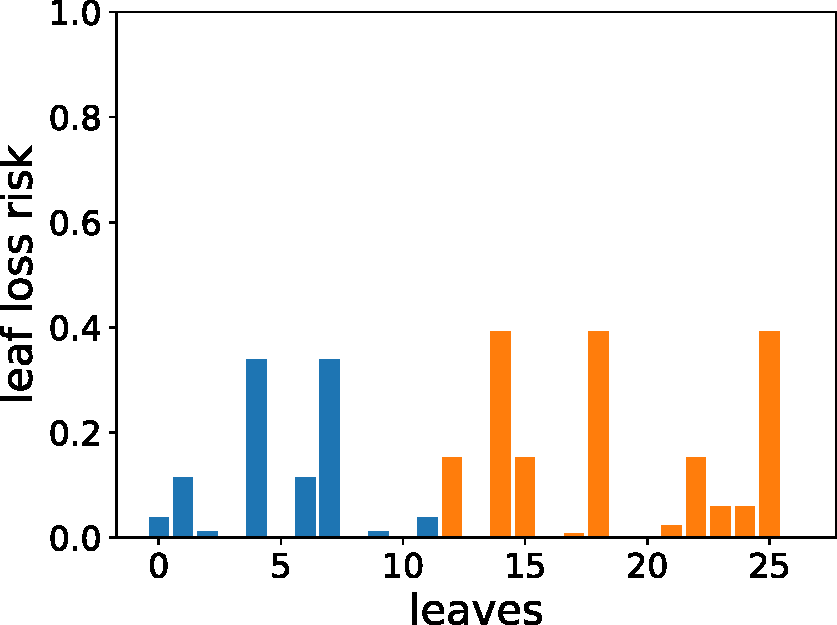
\includegraphics[width=\ratio\linewidth]{leaf_loss_NTarget200_Lambda1.pdf}\\
            {\small(a)\; Balanced data with 200 instances}
        \end{minipage}\vspace{0.2cm}
        \begin{minipage}[t]{\ratiob\linewidth}\vspace{0pt}
            \centering
            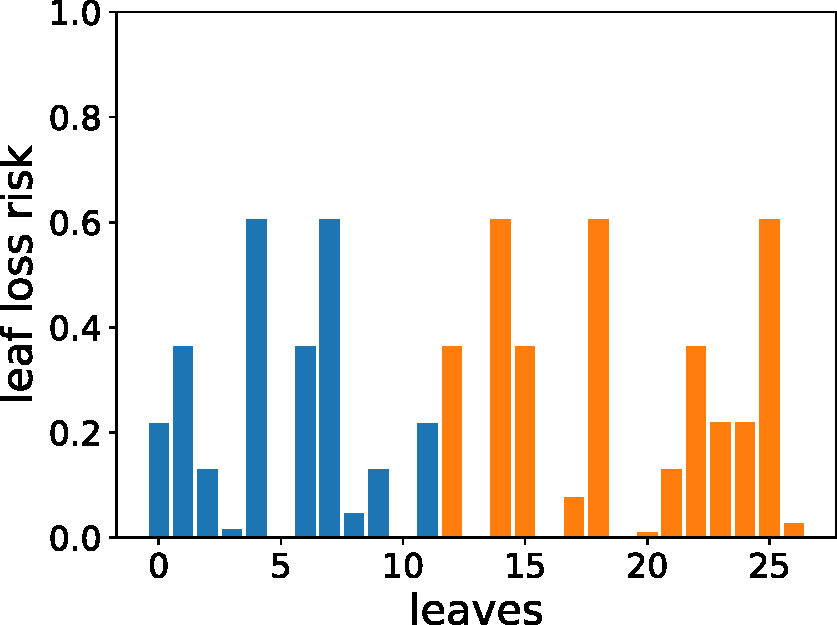
\includegraphics[width=\ratio\linewidth]{leaf_loss_NTarget100_Lambda1.pdf}\\
            {\small(b)\; Balanced data with 100 instances }
        \end{minipage}
        % \hfill
        \\
        \begin{minipage}[t]{\ratiob\linewidth}\vspace{0pt}
            \centering
            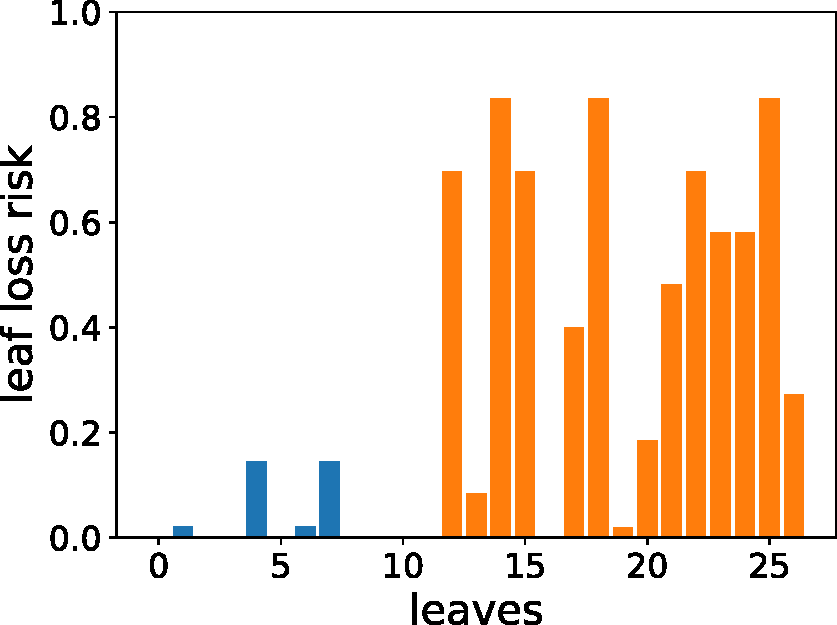
\includegraphics[width=\ratio\linewidth]{leaf_loss_NTarget200_Lambda01.pdf}\\
            {\small (c)\; Imbalanced data (10\% ratio) with 200 instances}
        \end{minipage}
        \centering
        \begin{minipage}[t]{\ratiob\linewidth}\vspace{0pt}
            \centering
            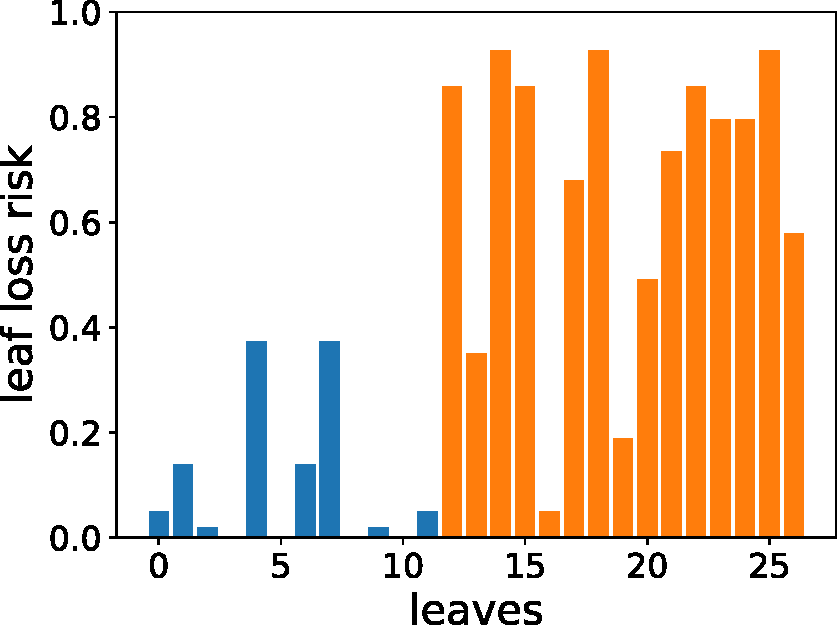
\includegraphics[width=\ratio\linewidth]{leaf_loss_NTarget100_Lambda01.pdf}\\
            {\small (d)\; Imbalanced data (10\% ratio) with 100 instances}
        \end{minipage}\vspace{0.1cm}
    \end{minipage}

\end{frame}

\subsection{SER for class imbalance}

\begin{frame}{SER for class imbalance}{\serr, \serll}
\begin{minipage}[t]{0.49\linewidth}
    \vspace{0pt}
    
    \centering
    \textbf{Structure Expansion and controlled Reduction}\\
        
    \renewcommand{\ratio}{0.8}
    \begin{overprint}
        \onslide<1>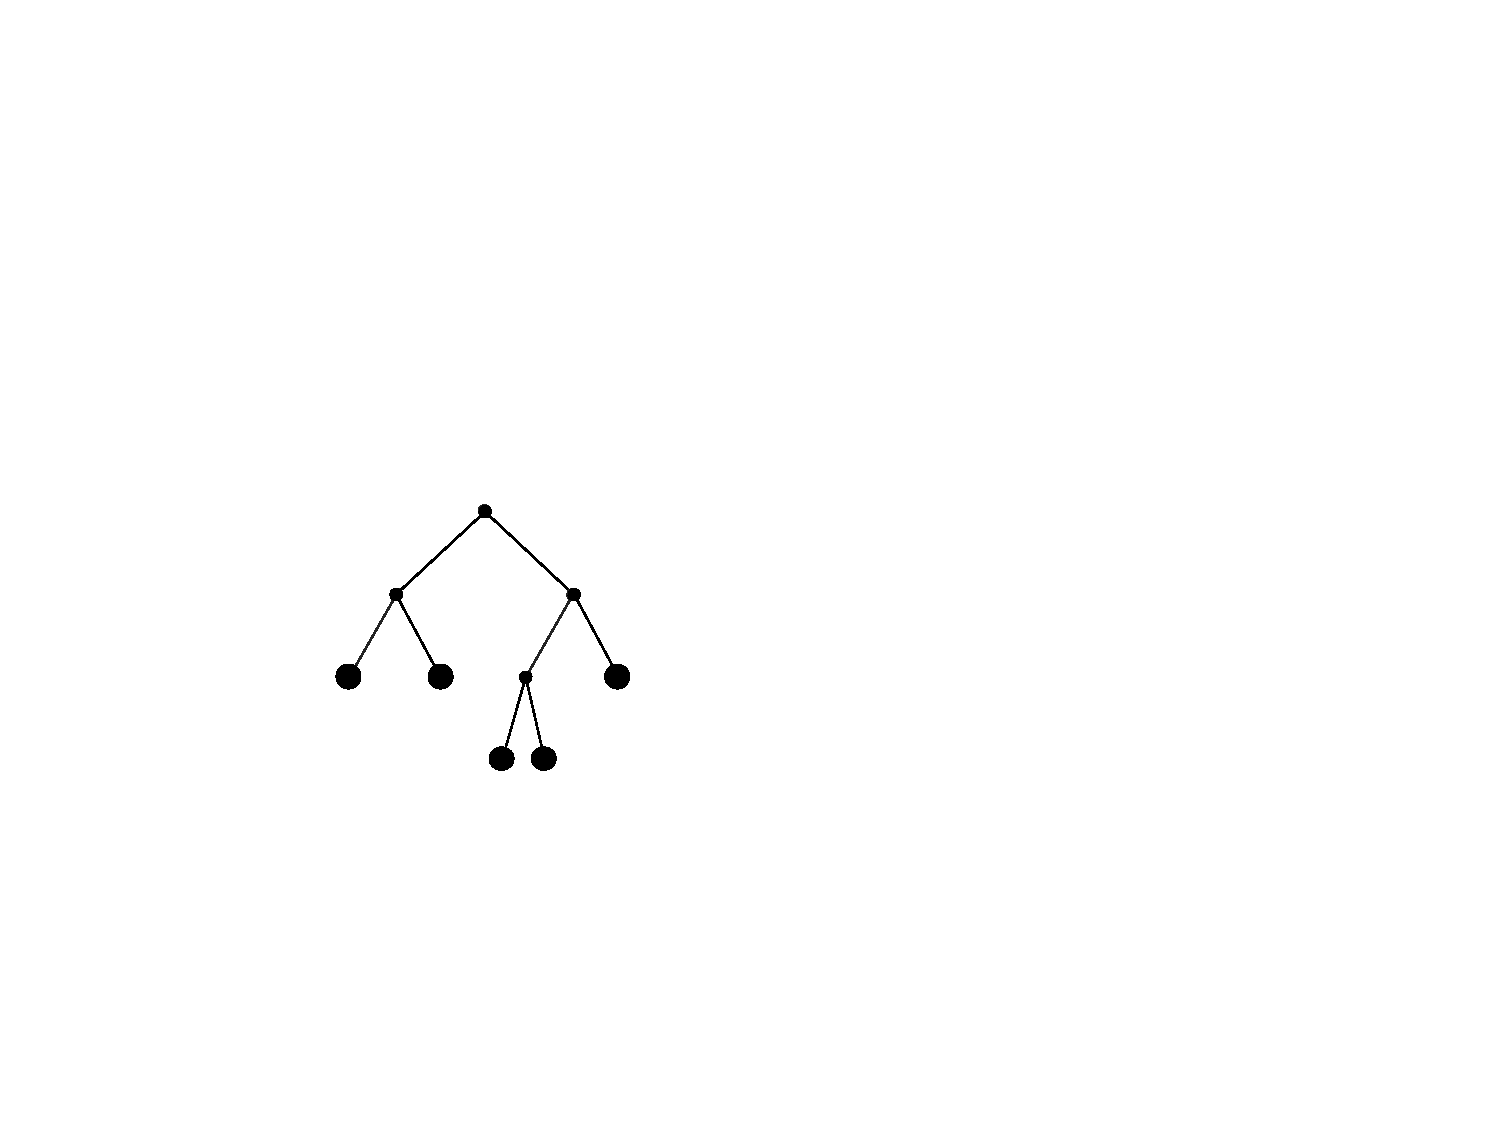
\includegraphics[width=\ratio\linewidth, trim={100 120 390 200}, clip]{schemas_ser_1.pdf}
        \onslide<2>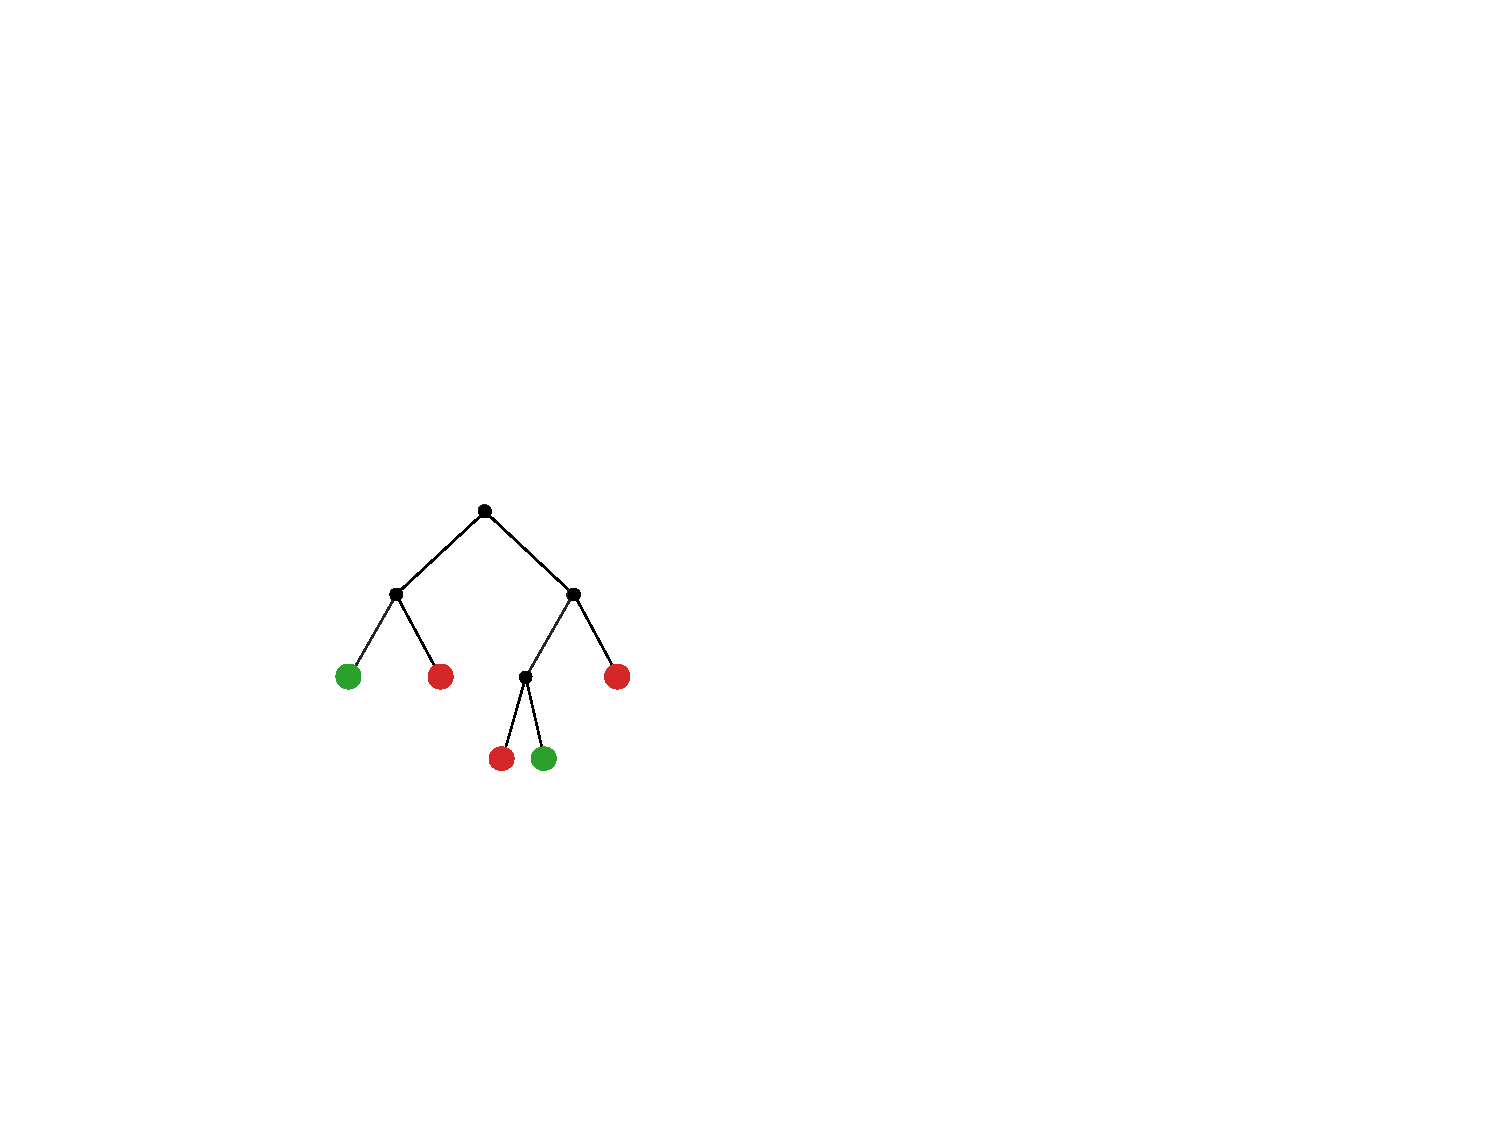
\includegraphics[width=\ratio\linewidth, trim={100 120 390 200}, clip]{schemas_sernr_1_15.pdf}
        \onslide<3>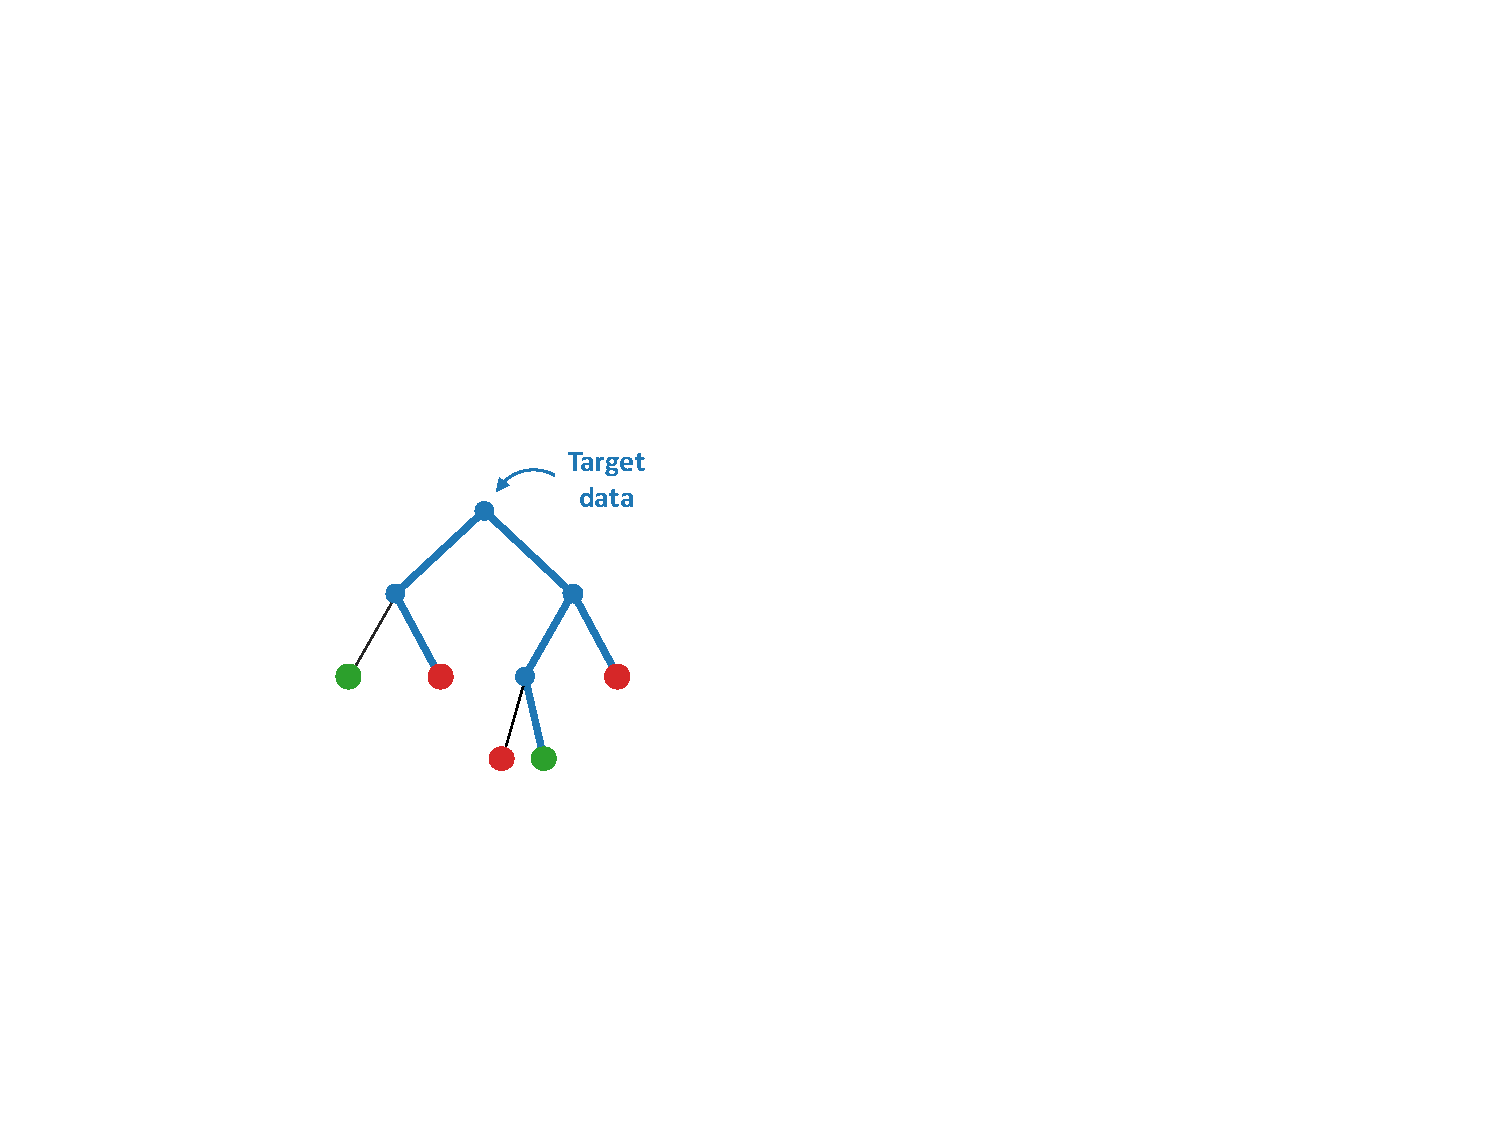
\includegraphics[width=\ratio\linewidth, trim={100 120 390 200}, clip]{schemas_sernr_2_15.pdf}
        \onslide<4>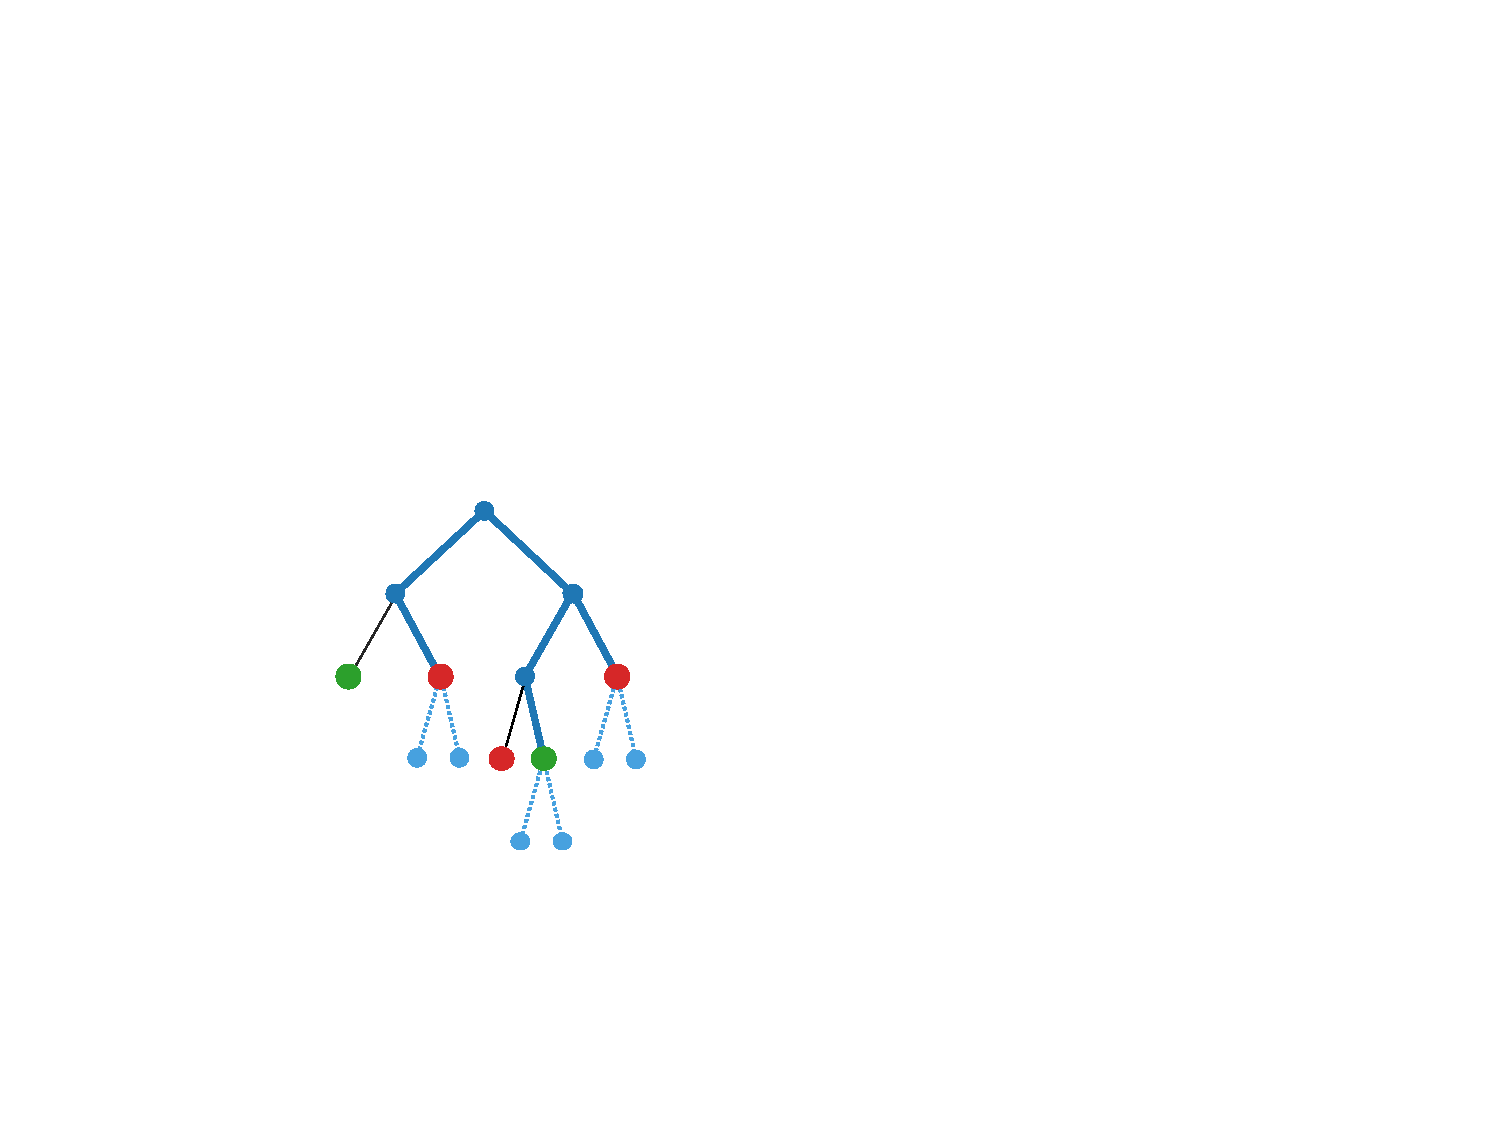
\includegraphics[width=\ratio\linewidth, trim={100 120 390 200}, clip]{schemas_sernr_3_15.pdf}
        \onslide<5>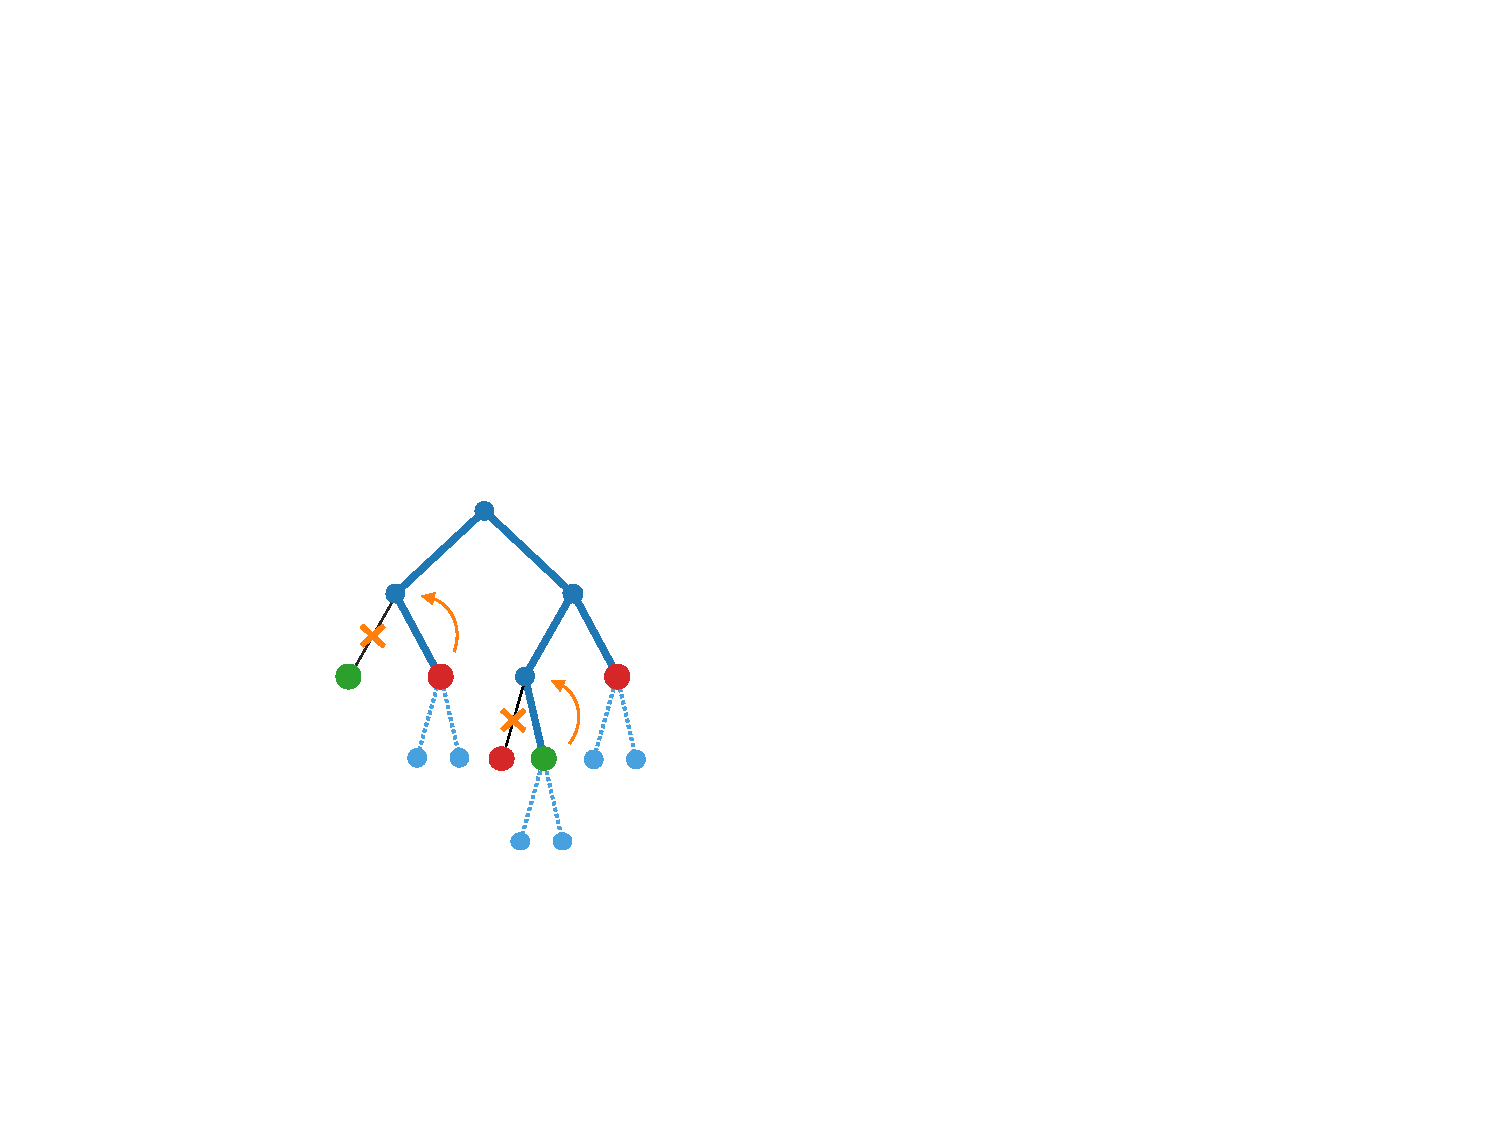
\includegraphics[width=\ratio\linewidth, trim={100 120 390 200}, clip]{schemas_sernr_4_15.pdf}
        \onslide<6>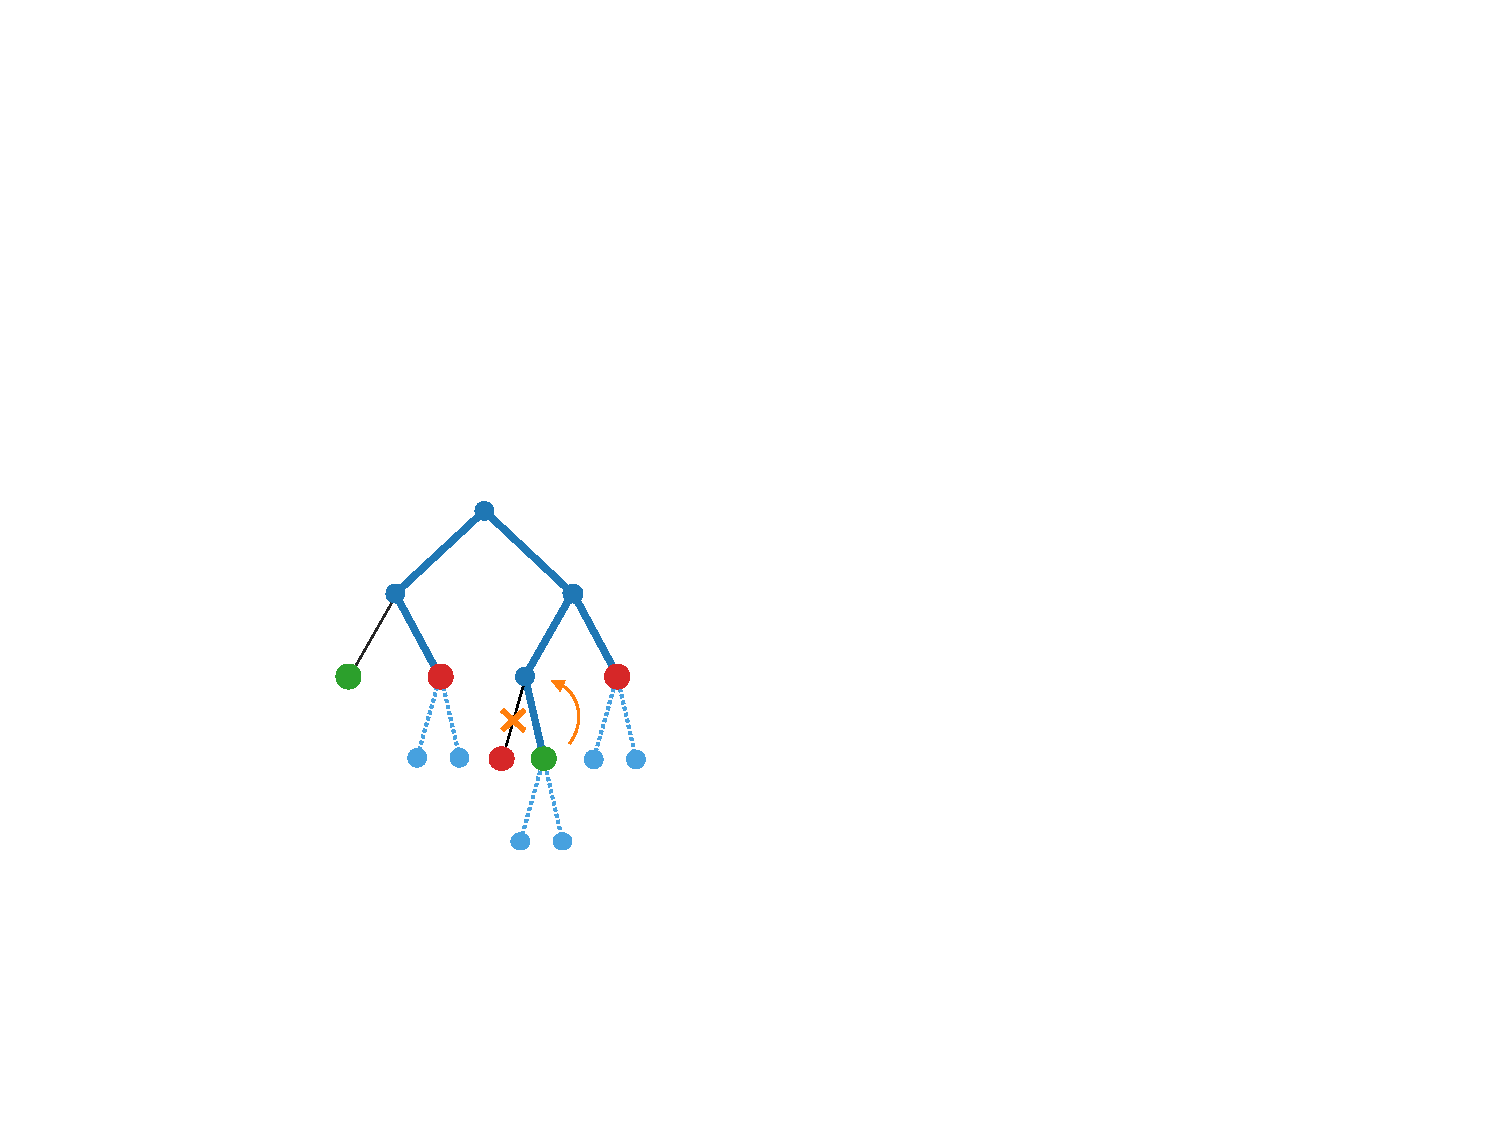
\includegraphics[width=\ratio\linewidth, trim={100 120 390 200}, clip]{schemas_sernr_5_15.pdf}
        \onslide<7->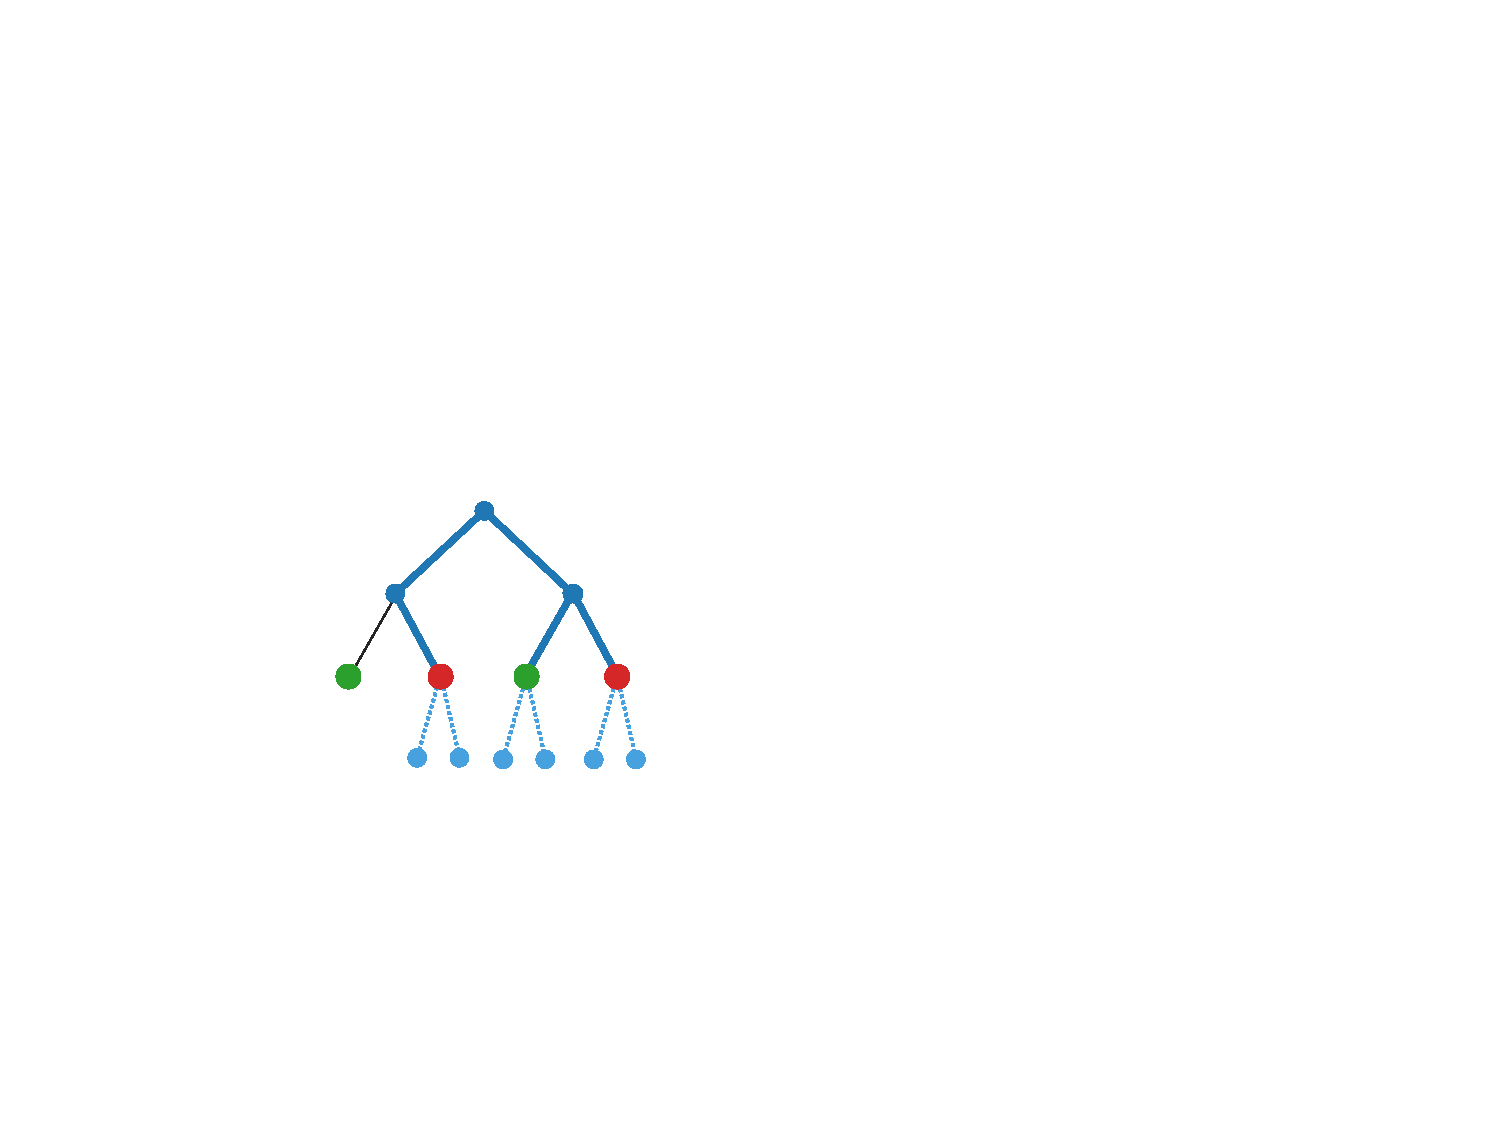
\includegraphics[width=\ratio\linewidth, trim={100 120 390 200}, clip]{schemas_sernr_6_15.pdf}
    \end{overprint}
    \pause
    \textcolor{mygreen}{\textbf{Minority class}}
\end{minipage}\hfill
\begin{minipage}[t]{0.49\linewidth}
    \vspace{0pt}
    \vspace{1.5cm}
    \begin{itemize}
    \pause \pause
    \item Expansion left unchanged
    \pause
    \item Reduction constrained
    \end{itemize}
\begin{minipage}[t]{0.49\linewidth}
    \vspace{0pt}
    \begin{tcolorbox}[title=\serr,size=title,boxrule=0.2pt]
    If node is of minority class, then no pruning
    \end{tcolorbox}
\end{minipage}
\begin{minipage}[t]{0.49\linewidth}
    \vspace{0pt}
    \begin{tcolorbox}[title=\serll,size=title,boxrule=0.2pt]
    If node is of minority class \textbf{and} still significant considering Target \textbf{and} $R_L > 0.5$, then no pruning
    \end{tcolorbox}
\end{minipage}


    

\end{minipage}

\end{frame}

\subsection{STRUT for class imbalance}

\begin{frame}{STRUT for class imbalance}{STRUT optimization}

\begin{minipage}[t]{0.4\linewidth}
    \vspace{0pt}
    
    \centering
    \textbf{STRUT: How are updated the new thresholds ?}\\

    \renewcommand{\ratio}{1.0}
    \begin{overprint}
        \onslide<1>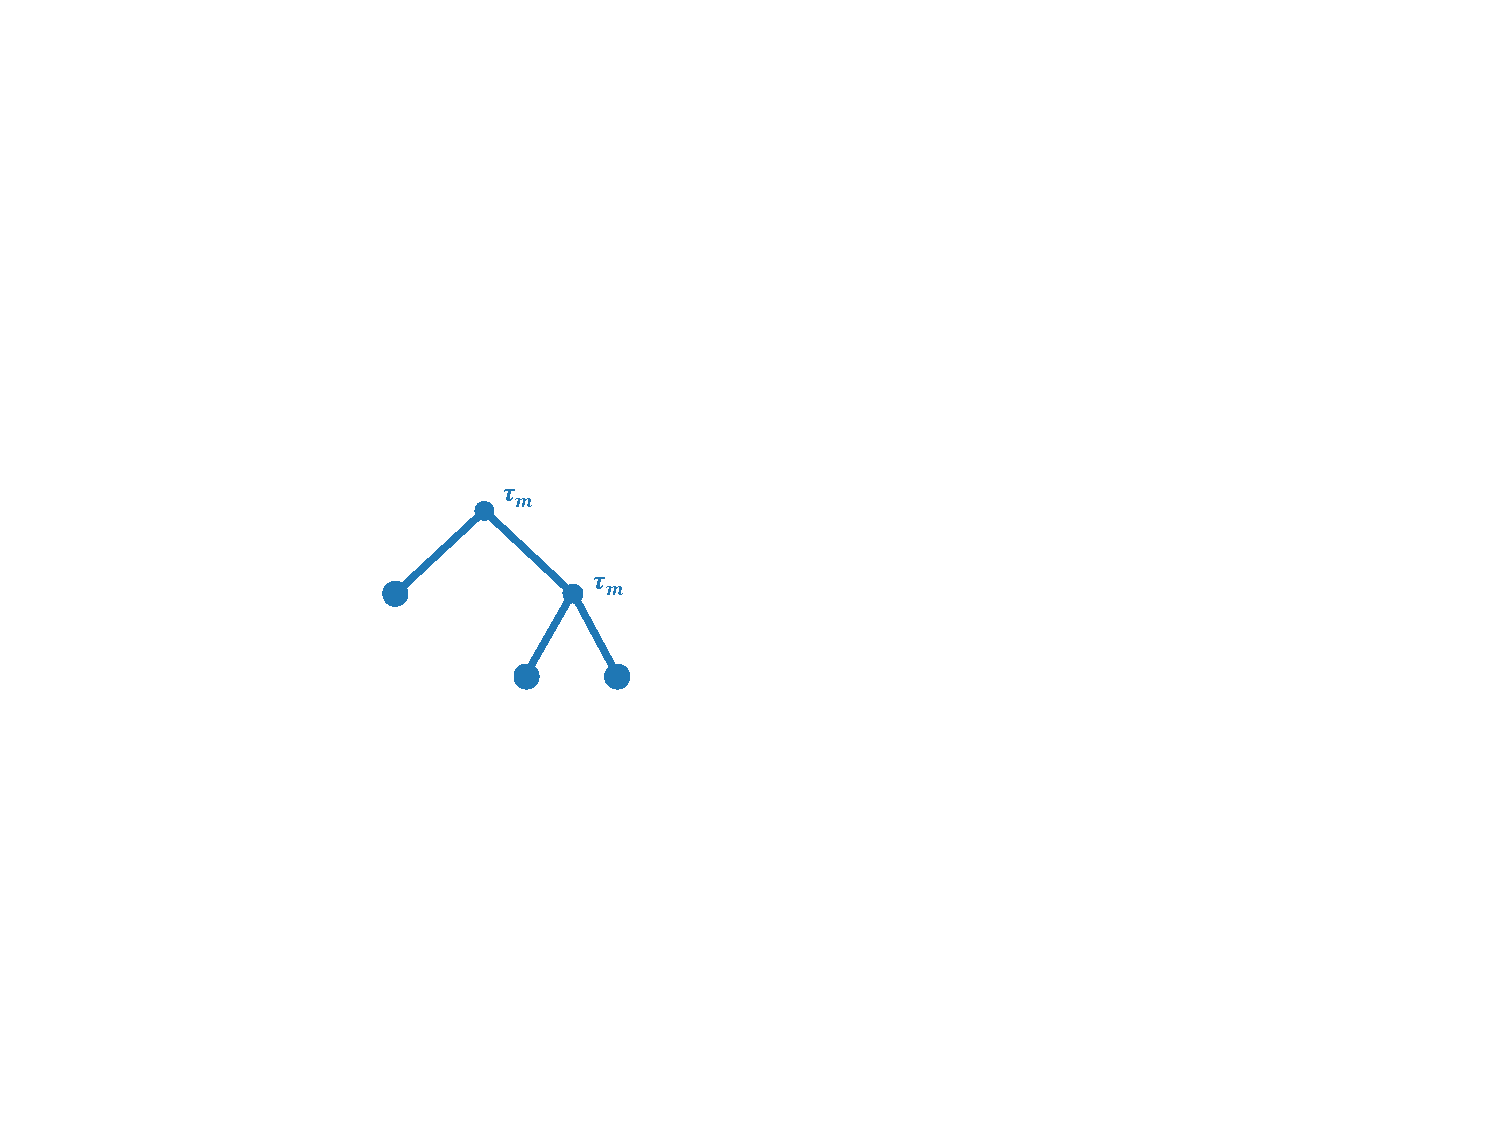
\includegraphics[width=\ratio\linewidth, trim={150 120 320 200}, clip]{schemas_strutoptim_0_15.pdf}
        \onslide<2>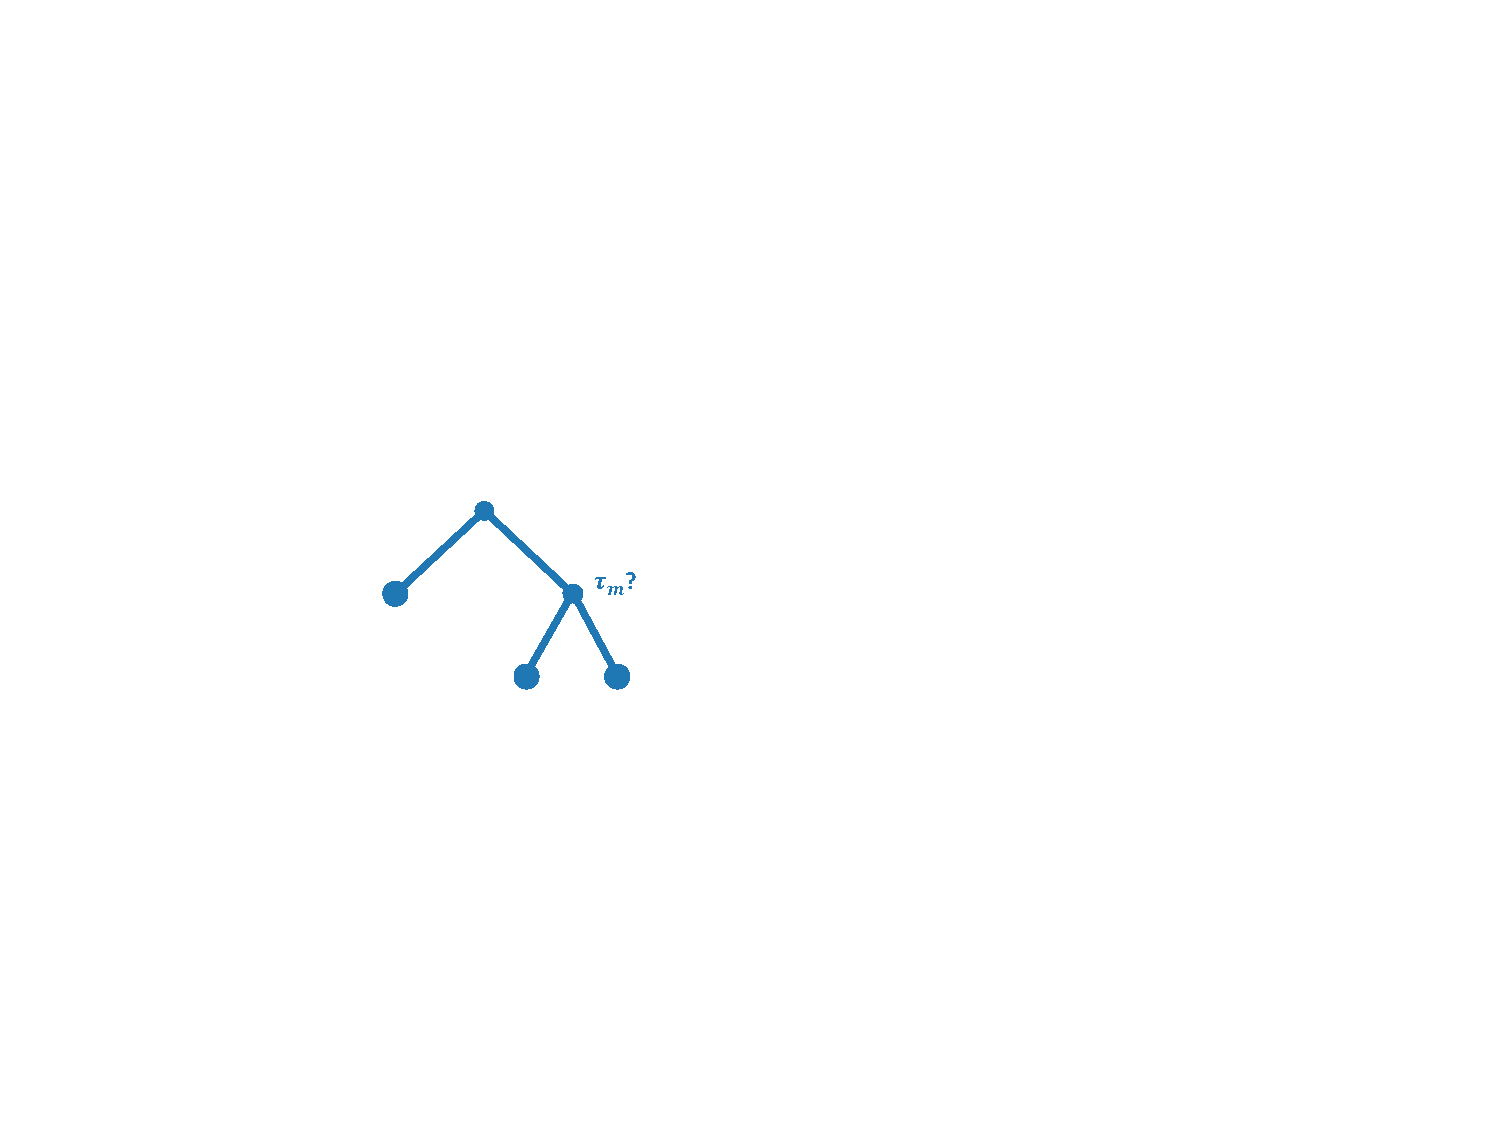
\includegraphics[width=\ratio\linewidth, trim={150 120 320 200}, clip]{schemas_strutoptim_1_15.pdf}
%         \onslide<3>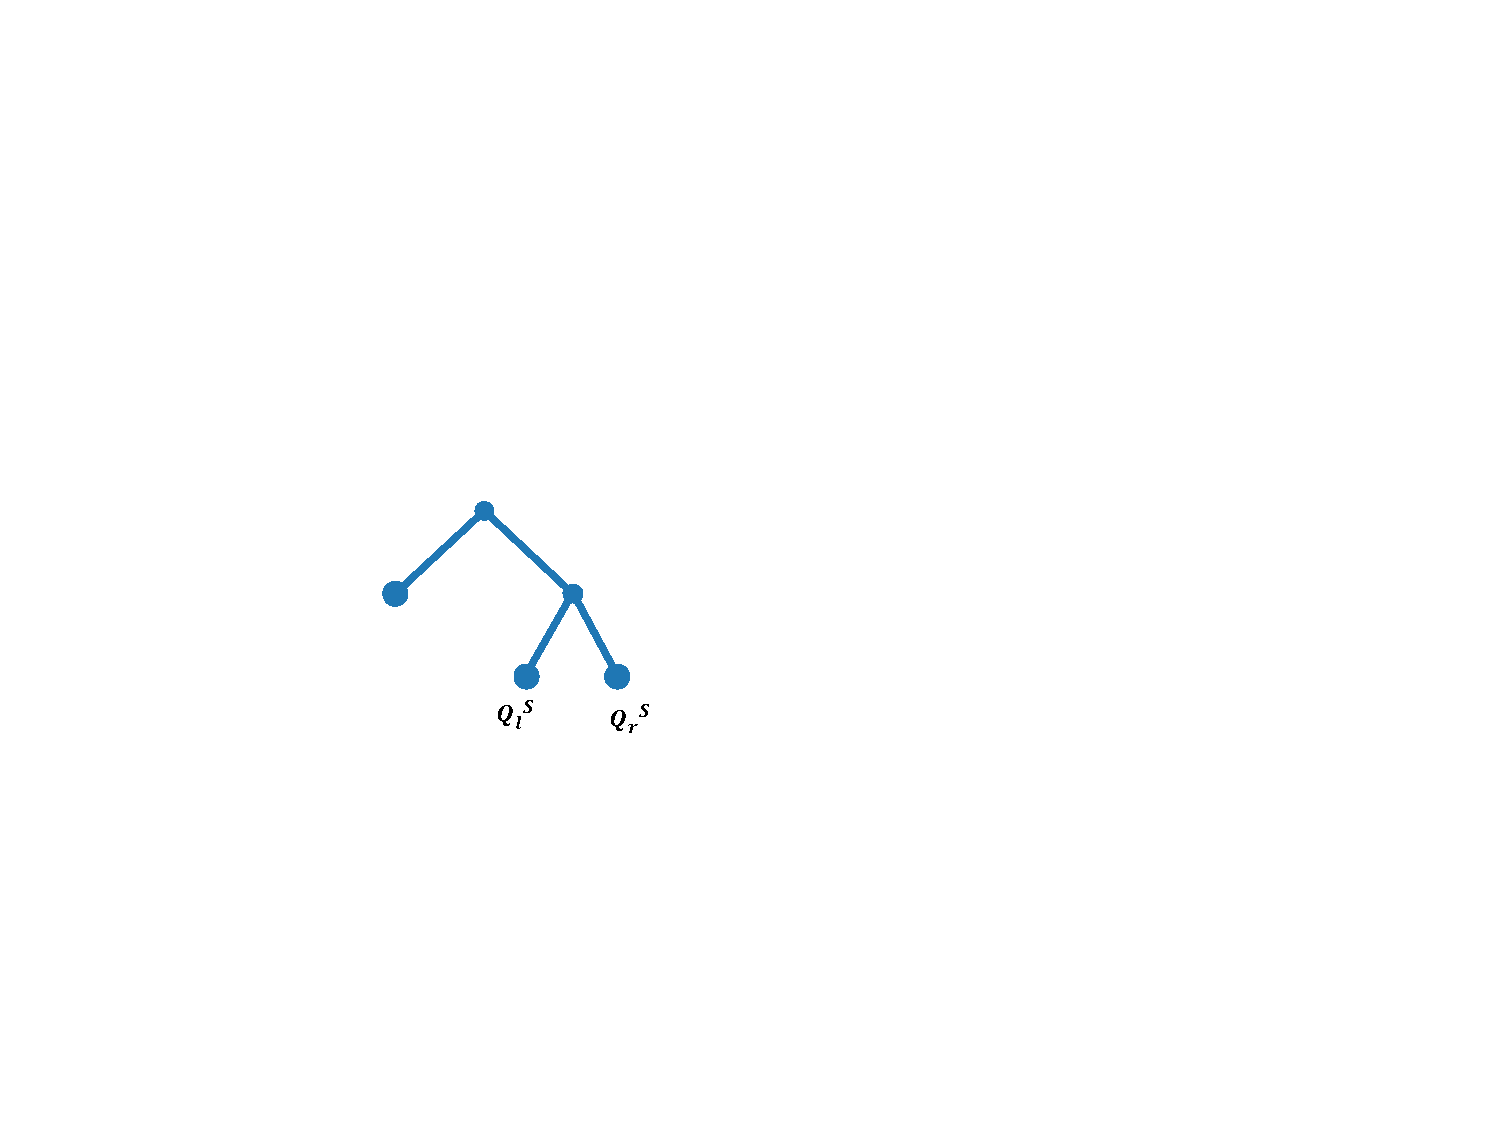
\includegraphics[width=\ratio\linewidth, trim={150 120 320 200}, clip]{schemas_strutoptim_2_15.pdf}
        \onslide<3->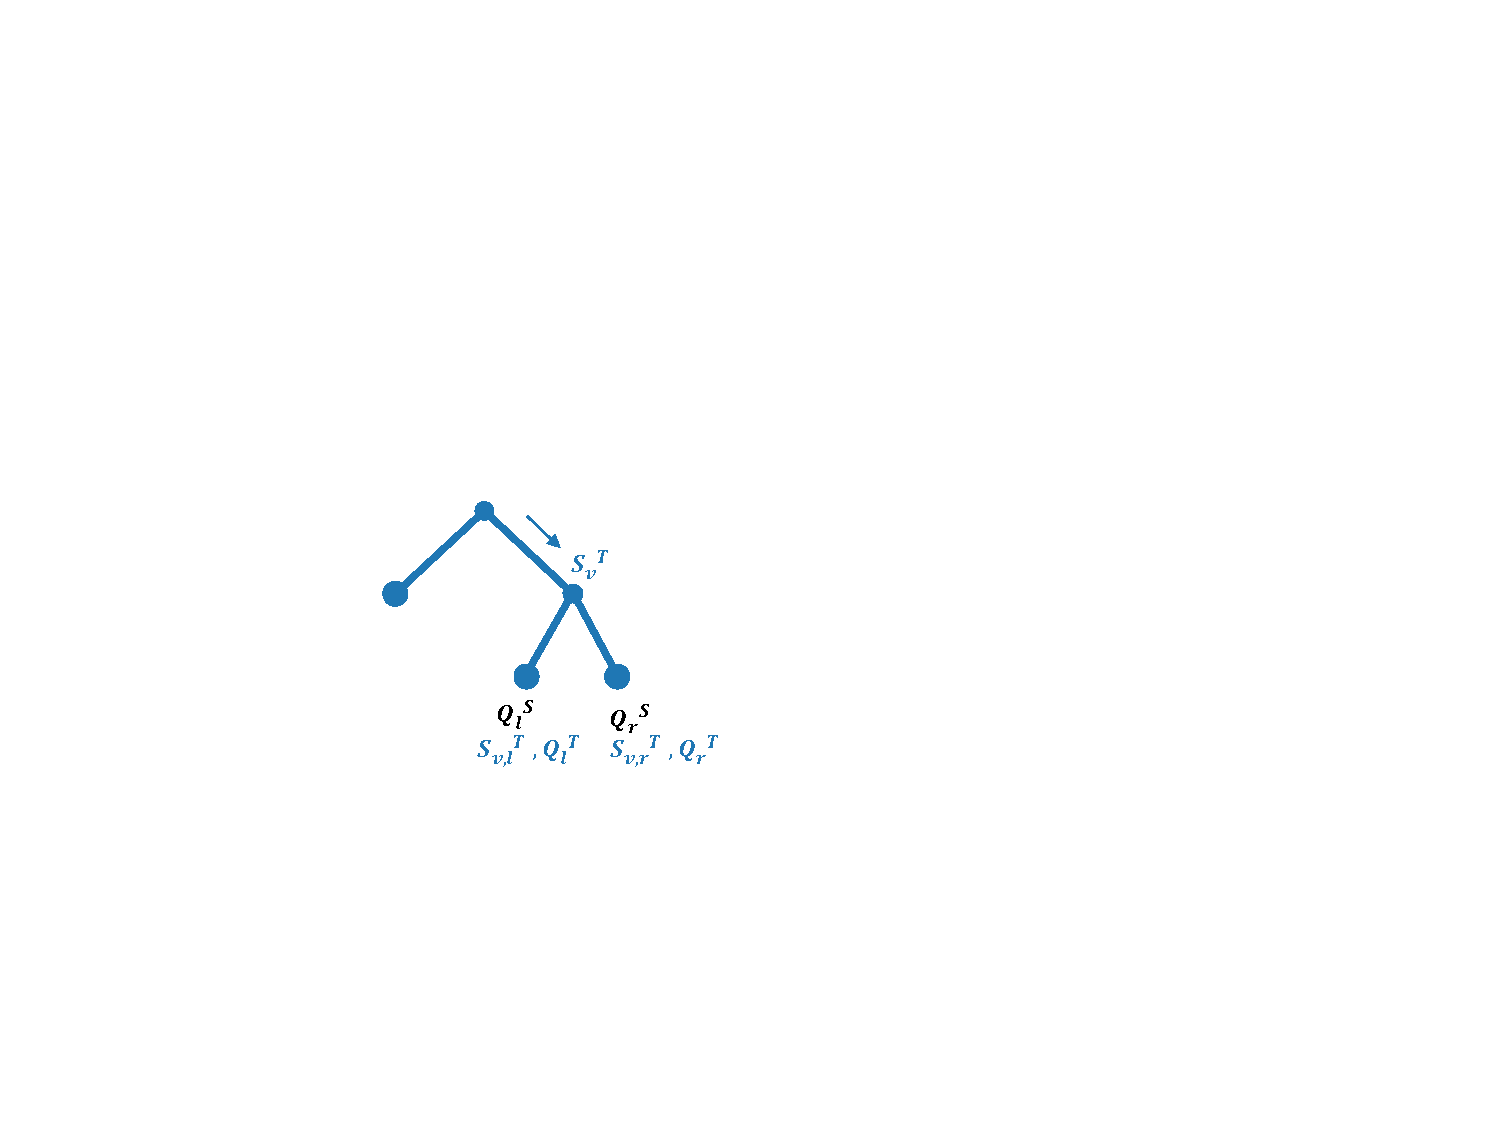
\includegraphics[width=\ratio\linewidth, trim={150 120 320 200}, clip]{schemas_strutoptim_3_15.pdf}
    \end{overprint}
\end{minipage}\hfill
\begin{minipage}[t]{0.55\linewidth}
    \vspace{0pt}
    \pause \pause
    $Q_{l}^{S}$, $Q_{r}^{S}$: class proportions of source data in children w.r.t.\ the \emph{original} split\\
%     \pause
    $S_{v,l}^{T}$, $S_{v,r}^{T}$: subsets of $S_{v}^{T}$ that fall in the children nodes of $v$\\
    $Q_{l}^{T}(\tau)$, $Q_{r}^{T}(\tau)$: class proportions of target data in children w.r.t.\ the \emph{new} split\\
%     \pause
    \textbf{Divergence Gain}: similarity between the original label distributions and the new ones
    $$
    DG\left(\tau\right) = 1 - \frac{|S_{v,l}^{T}|}{|S_{v}^{T}|}JSD(Q_{l}^{S}, Q_{l}^{T})
    - \frac{|S_{v,r}^{T}|}{|S_{v}^{T}|}JSD(Q_{r}^{S}, Q_{r}^{T})
    $$
    \small
    Jensen-Shannon divergence:
    $$JSD(P, Q) = \frac{1}{2}\left(D_{KL}(P||M) + D_{KL}(Q||M)\right) $$
    \begin{flushright}
    $M = \frac{1}{2} \left(P +Q\right) $
    \end{flushright}
    Kullback-Leibler divergence:
    $$D_{KL}(P||Q) = \sum_{k}{P(k)\ln\left(\frac{P(k)}{Q(k)}\right)}$$
\end{minipage}

\end{frame}

% \subsection{STRUT for class imbalance}

\begin{frame}{STRUT for class imbalance}{STRUT optimization}
\begin{minipage}[t]{0.4\linewidth}
    \vspace{0pt}
    \centering
    \textbf{STRUT: How are updated the new thresholds ?}\\
    \renewcommand{\ratio}{1.0}
    \begin{overprint}
%         \onslide<1>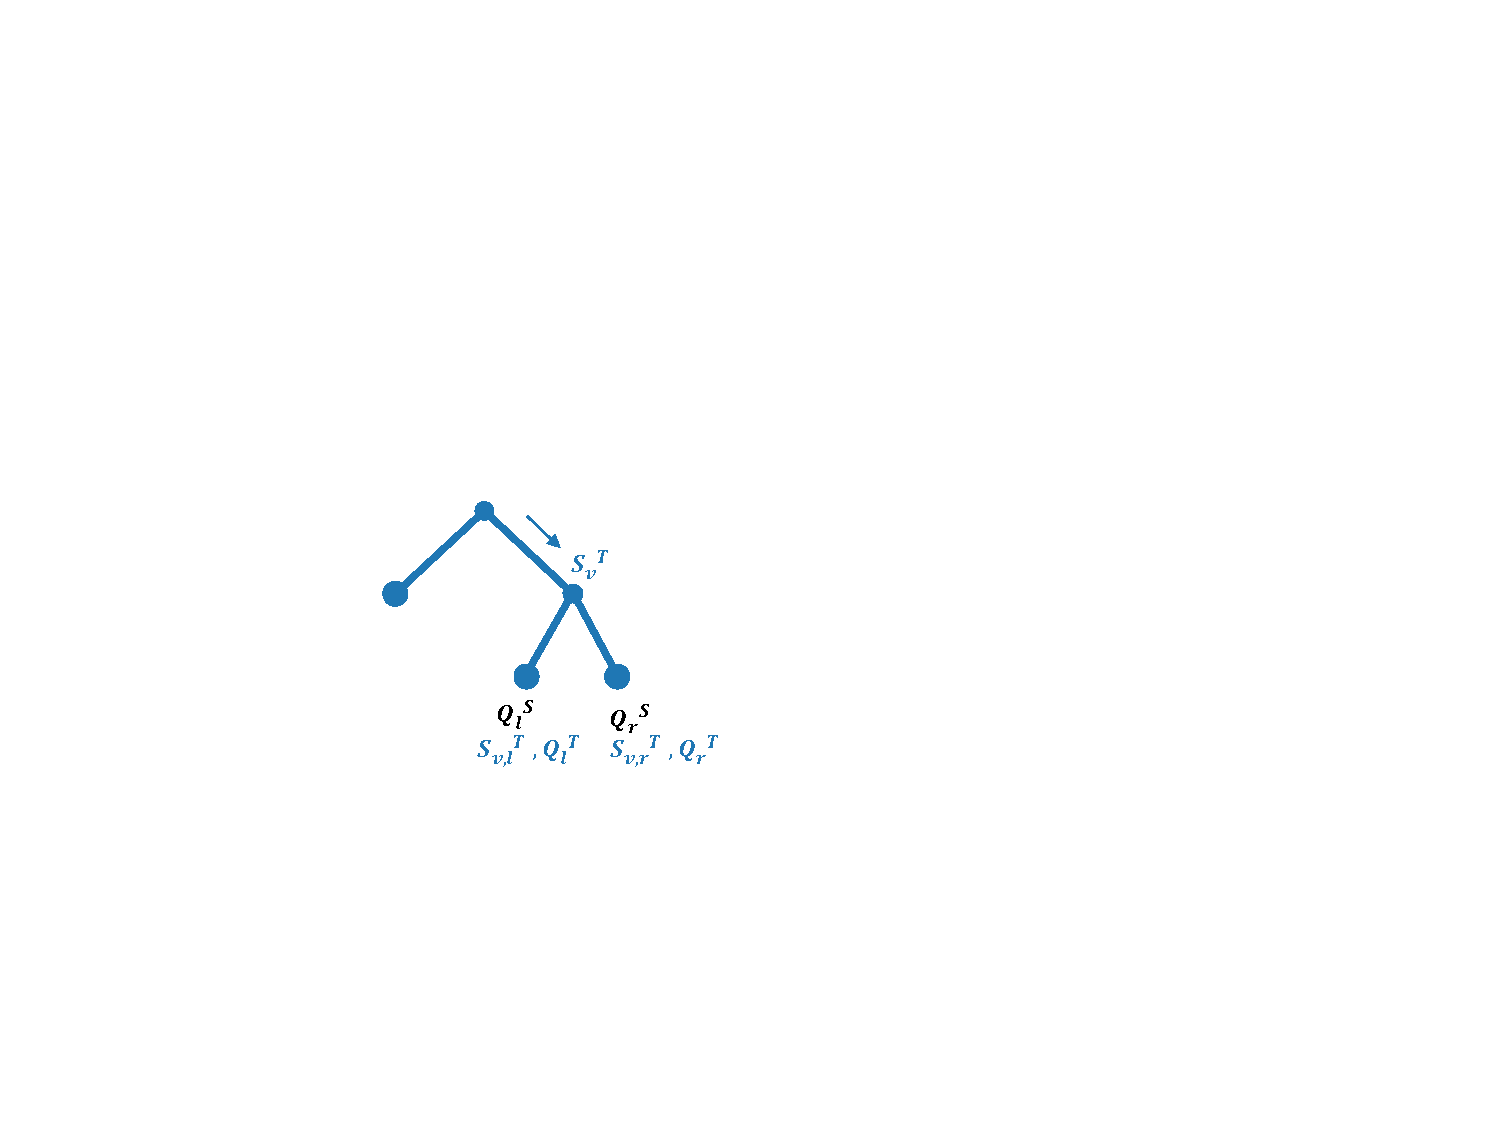
\includegraphics[width=\ratio\linewidth, trim={150 120 320 200}, clip]{schemas_strutoptim_3_15.pdf}
%         \onslide<2>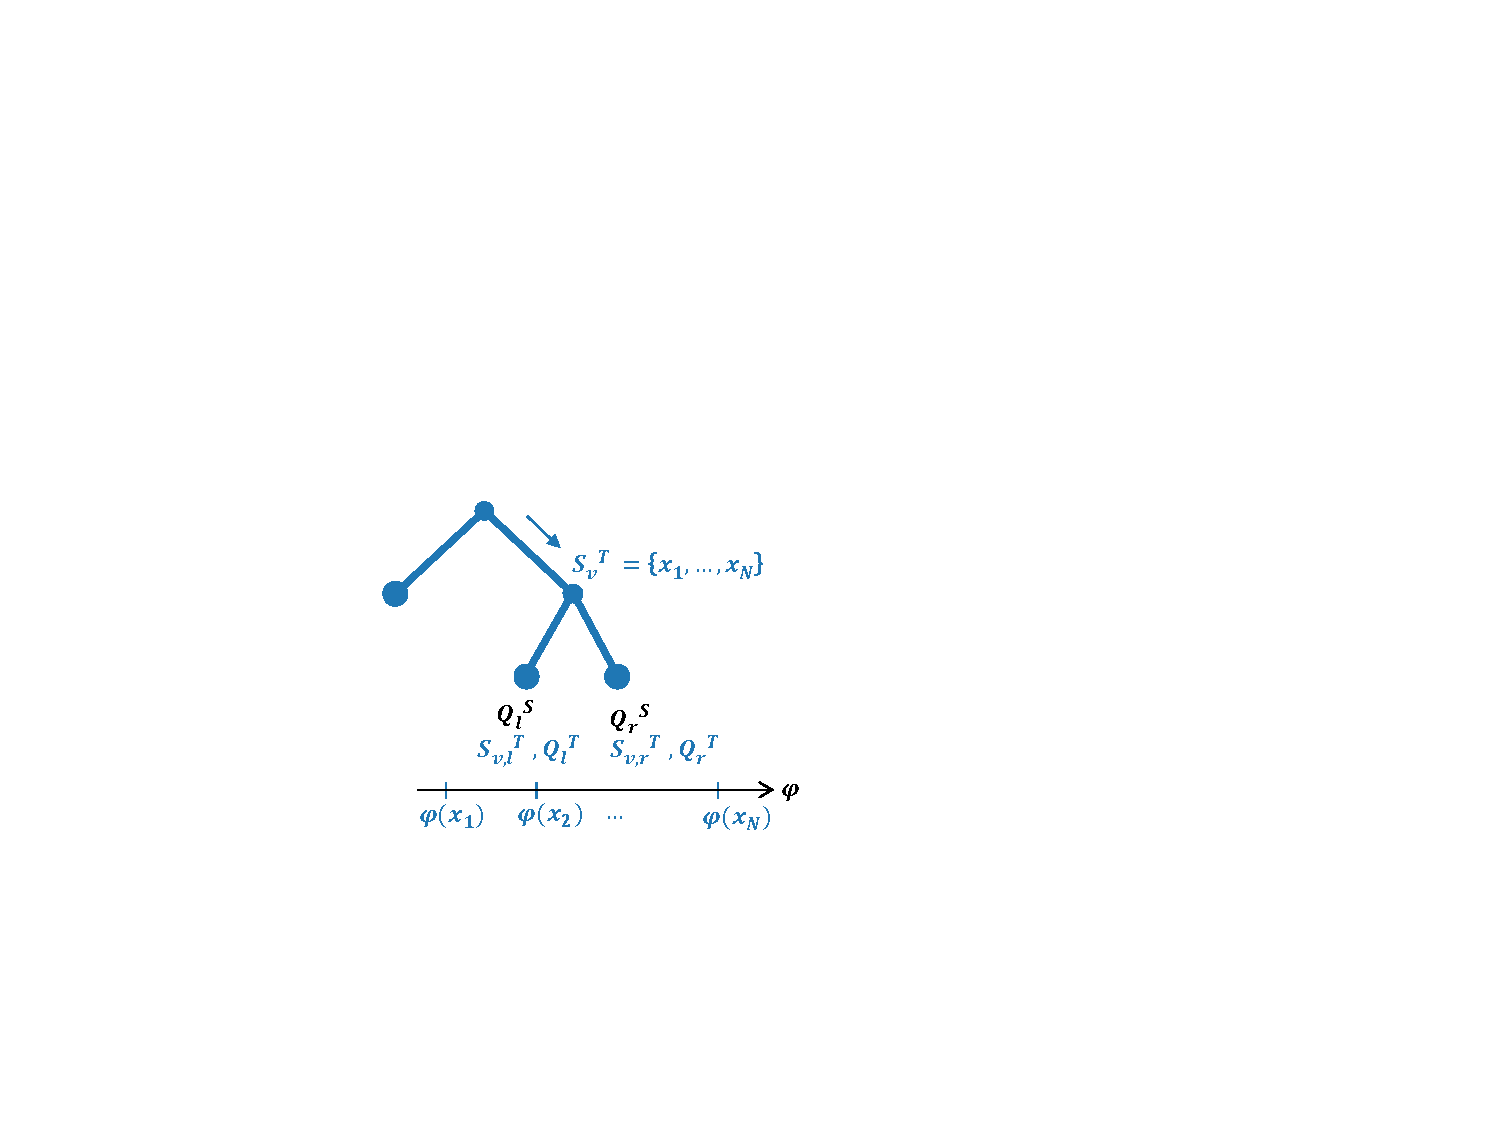
\includegraphics[width=\ratio\linewidth, trim={150 120 320 200}, clip]{schemas_strutoptim_4_15.pdf}
        \onslide<1->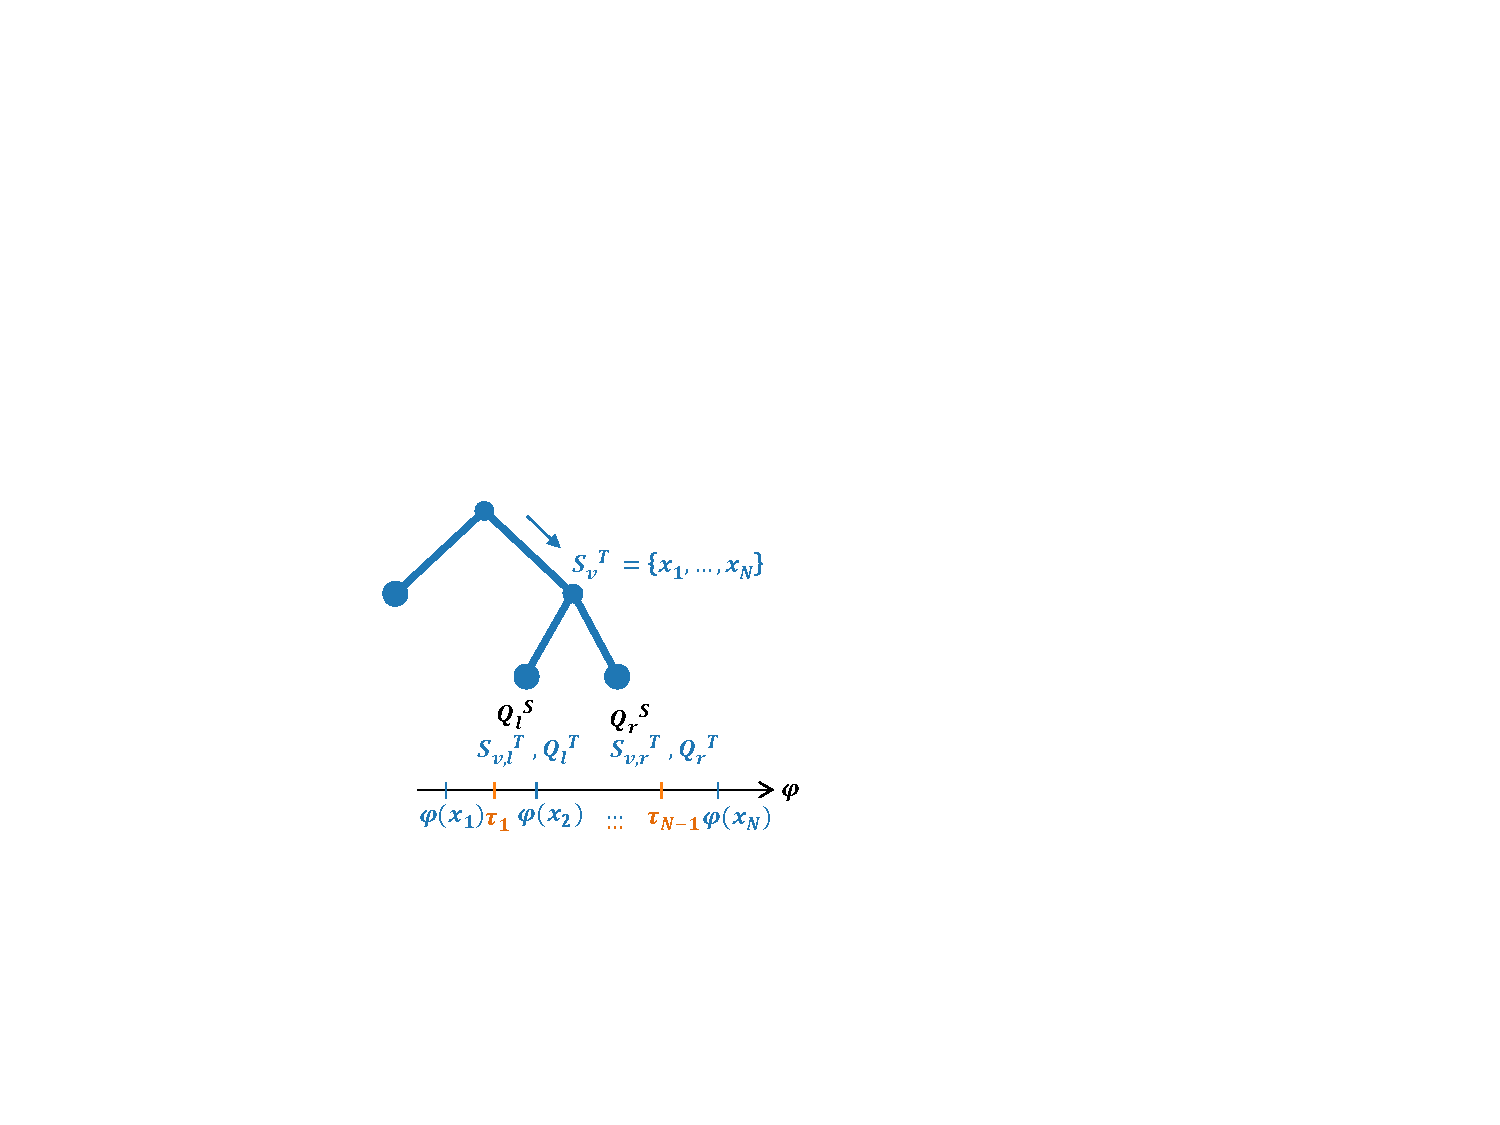
\includegraphics[width=\ratio\linewidth, trim={150 120 320 200}, clip]{schemas_strutoptim_5_15.pdf}
    \end{overprint}
\end{minipage}\hfill
\begin{minipage}[t]{0.55\linewidth}
    \vspace{0pt}
    
    \textbf{Goal: } Maximize DG while being in a local maximum of Information Gain (IG) (here IG = Gini gain)
%     \pause \pause \pause
    \begin{align*}
        &\tau_{m} = \argmax_{\tau \in \mathrm{T}_{v}}\left(DG\left(  \tau ,  Q_{l}^{T}(\tau), Q_{r}^{T}(\tau)\right)\right) \\
        &\text{s.t.\ } IG(\tau_{m-1}) < IG(\tau_{m}) \text{ and } IG(\tau_{m}) > IG(\tau_{m+1})
    \end{align*}
    \vspace{1cm}

    \pause
    \begin{itemize}
        \item  $Q^S$ have less meaning when going deeper
        \item  Do we really want to keep $Q^S$ and $Q^T$ close ?
    \end{itemize}
\end{minipage}

\end{frame}

\begin{frame}{STRUT for class imbalance}{\strutnd, \struthi}

    \begin{tcolorbox}[title=\strutnd,size=title,boxrule=0.2pt]
    STRUT without DG: maximization of IG
    \end{tcolorbox}
    \pause
    \begin{tcolorbox}[title=\struthi,size=title,boxrule=0.2pt]
    Framework of homogeneous class imbalance, use
    % \begin{equation}
    % p^T(y/x) = \lambda_y\frac{ p^S(y/x)}{\sum \limits_{y'}{ \lambda_{y'}p^S(y'/x)}} 
    % \label{probcond}
    % \end{equation}
    \begin{align*}
        & p^T(y/x) = \lambda_y \frac{p^S(y/x)}{\int{\lambda_y p^S(y/x)dy}}
    %       & \textrm{with} \quad \lambda_y = \frac{P_y^T}{P_y^S} 
    \end{align*}
    %      \flushright $\textrm{with} \quad \lambda_y = \frac{P_y^T}{P_y^S}$\ref{eq:}
    to change the source class proportions in DG:
    \begin{equation*}
    {Q_l^S} ' = \lambda_k\frac{ Q_l^S}{\sum \limits_{k}{ \lambda_{k}Q_l^S}} \quad \quad
    {Q_r^S} ' = \lambda_k\frac{ Q_r^S}{\sum \limits_{k}{ \lambda_{k}Q_r^S}} 
%     \label{probcond}
    \end{equation*}
    \end{tcolorbox}
    \pause
    \centering \textcolor{myorange}{\struthi} can be seen as a generalization of STRUT
 
\end{frame}

\subsection{Results}

\begin{frame}{Results}{Synthetic data}
    
% \centering
\begin{minipage}[t]{0.49\linewidth}
    \vspace{0pt}
    \textbf{Gaussian generator}\\
    Source dataset: combination of several multivariate Gaussian clusters.
    We use $N_\text{source} = 200$ and $N_{clust} = 10$.
    Initial parameters are randomly drawn from Uniform distribution: $\mu_i \in [-70,70]$ and $\sigma_i \in [5,15]$
    % For each class $k$ with $N_k$ clusters of this class :
    % $$ C^k = \{  \mathcal{N}(\mu_1,\sigma_1),..., \mathcal{N}(\mu_{N_k},\sigma_{N_k} )\}$$ 
    % $$  \forall k, (X,Y = k) \sim \sum_{j=1}^{N_k}  w_j^k \mathcal{N}(\mu_j,\sigma_j)$$
\end{minipage}\hfill
\begin{minipage}[t]{0.49\linewidth}
    \vspace{0pt}
    \textbf{Transformations}\\
    Basic transformations on Source clusters are applied to get a Target dataset:
    \begin{itemize}
        \item Drifts  \, ($\mu_i$)
        \item Stretch / Squeeze \, ($\sigma_i$)
        \item Adding / Remove clusters
    \end{itemize}
    Transformations are combined with imbalance ratio (from 2\% to 50\%), and $N_\text{target} = 1000$
\end{minipage}

\bigskip
\centering
\begin{minipage}[t]{0.7\linewidth}
    \vspace{0pt}
    \renewcommand{\ratio}{0.32}
    \renewcommand{\ratiob}{0.85}
    \begin{minipage}[t]{\ratio\linewidth}\vspace{0pt}
        \centering
        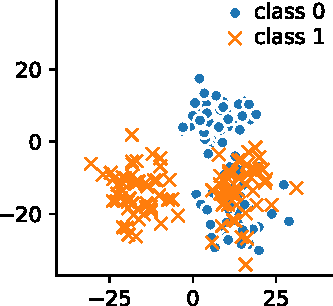
\includegraphics[width=\ratiob\linewidth]{Source_D_2_C_3_N_200_Target_drift_deg_10_imb_10_Source_2_epure.pdf}\\
        {\small Source data...}
    \end{minipage}
    \begin{minipage}[t]{\ratio\linewidth}\vspace{0cm}
        \centering
        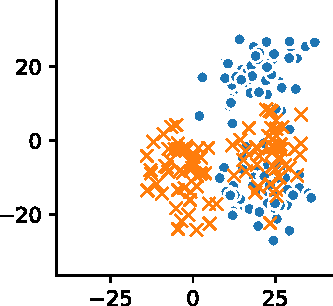
\includegraphics[width=\ratiob\linewidth]{Source_D_2_C_3_N_200_Target_drift_deg_10_imb_10_AfterDrift_2_epure.pdf}\\
        {\small ...after a drift...}
    \end{minipage}
    \begin{minipage}[t]{\ratio\linewidth}\vspace{0cm}
        \centering
        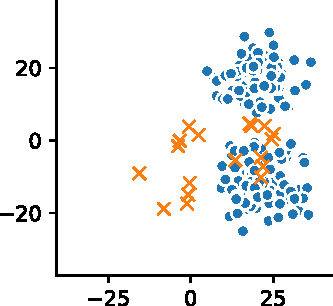
\includegraphics[width=\ratiob\linewidth]{Source_D_2_C_3_N_200_Target_drift_deg_10_imb_10_AfterImb_2_epure.pdf}\\
        {\small ...and homogeneous imbalance}
    \end{minipage}
\end{minipage}

\end{frame}

\begin{frame}{Results}{Synthetic data}

\centering
% \textbf{Synthetic data}

    \renewcommand{\ratio}{0.9}
%         \centering
        \begin{minipage}[t]{0.33\linewidth}\vspace{0pt}
            \centering
            \begin{minipage}[t]{\ratio\linewidth}\vspace{0pt}
            \centerline{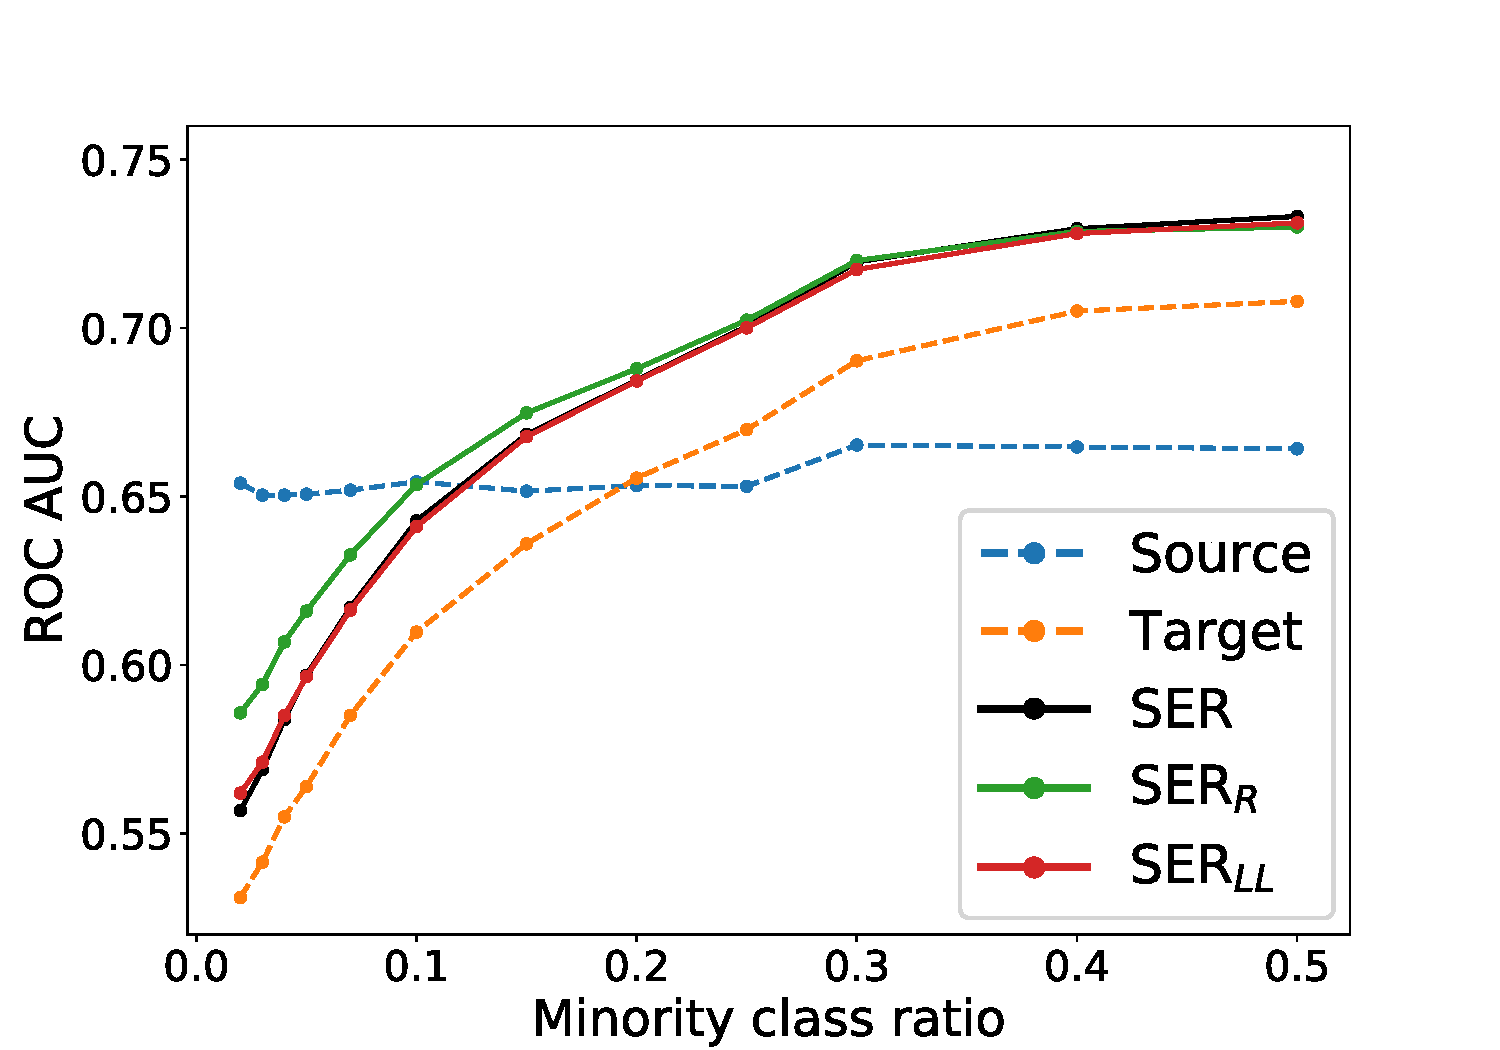
\includegraphics[width=\linewidth, trim={0 0 0 50}, clip]{SER_ll_05_DataSYNTH_Source_D_3_C_10_N_200_Target_drift_deg_5_Scorefilescores_2020_02_22_BALANCESOURCE50_KFOLD_NTARGET150_NB_TREE1_BarPlot_AUC_depthNone_bigleg.pdf}}
            \end{minipage}\\
            \begin{minipage}[t]{\ratio\linewidth}\vspace{0cm}
            \centerline{\includegraphics[width=\linewidth, trim={0 0 0 40}, clip]{STRUT_DataSYNTH_Source_D_3_C_10_N_200_Target_drift_deg_5_Scorefilescores_2020_02_22_BALANCESOURCE50_KFOLD_NTARGET150_NB_TREE1_BarPlot_AUC_depthNone_bigleg.pdf}}
            \end{minipage}\\
            \medskip
            {\small(a)\; Drift}
        \end{minipage}
        \begin{minipage}[t]{0.33\linewidth}\vspace{0pt}
            \centering
            \begin{minipage}[t]{\ratio\linewidth}\vspace{0pt}
            \centerline{\includegraphics[width=\linewidth, trim={0 0 0 50}, clip]{SER_ll_05_DataSYNTH_Source_D_3_C_10_N_200_Target_std_deg_9_Scorefilescores_2020_02_19_3_synth_BALANCESOURCE50_KFOLD_NTARGET150_NB_TREE1_BarPlot_AUC_depthNone_noleg.pdf}}
            \end{minipage}\\
            \begin{minipage}[t]{\ratio\linewidth}\vspace{0cm}
            \centerline{\includegraphics[width=\linewidth, trim={0 0 0 40}, clip]{STRUT_DataSYNTH_Source_D_3_C_10_N_200_Target_std_deg_9_Scorefilescores_2020_02_19_3_synth_BALANCESOURCE50_KFOLD_NTARGET150_NB_TREE1_BarPlot_AUC_depthNone_noleg.pdf}}
            \end{minipage}\\
            \medskip
            {\small(b)\; Stretch / Squeeze}
        \end{minipage}
        \begin{minipage}[t]{0.33\linewidth}\vspace{0pt}
            \centering
            \begin{minipage}[t]{\ratio\linewidth}\vspace{0pt}
            \centerline{\includegraphics[width=\linewidth, trim={0 0 0 50}, clip]{SER_ll_05_DataSYNTH_Source_D_3_C_10_N_200_Target_add_remove_deg_0_Scorefilescores_2020_02_20_2_synth_BALANCESOURCE50_KFOLD_NTARGET150_NB_TREE1_BarPlot_AUC_depthNone_noleg.pdf}}
            \end{minipage}\\
            \begin{minipage}[t]{\ratio\linewidth}\vspace{0cm}
            \centerline{\includegraphics[width=\linewidth, trim={0 0 0 40}, clip]{STRUT_DataSYNTH_Source_D_3_C_10_N_200_Target_add_remove_deg_0_Scorefilescores_2020_02_20_2_synth_BALANCESOURCE50_KFOLD_NTARGET150_NB_TREE1_BarPlot_AUC_depthNone_noleg.pdf}}
            \end{minipage}\\
            \medskip
            {\small(c)\; Add / Remove}
        \end{minipage}

\begin{itemize}
    \item Strong imbalance leads to negative transfer
    % COM: mais expereience avec transfo plus violente font que le transfer est tt le temps + interessant
    \item SER: \serll\ close to SER, \serr\ better than SER (esp. with high imbalance)
    \item STRUT: both variants beat the original STRUT
\end{itemize}

    
\end{frame}

\begin{frame}{Results}{Public data}

\centering
Two real data sets where the imbalance ratio is controlled with downsampling.

% \textbf{Real data}

\renewcommand{\ratio}{0.9}
        \centering
        \begin{minipage}[t]{0.33\linewidth}\vspace{0pt}
            \centering
            \begin{minipage}[t]{\ratio\linewidth}\vspace{0pt}
            \centerline{\includegraphics[width=\linewidth, trim={0 0 0 50}, clip]{SER_ll_05_Datamagic_gamma_telescope_Scorefilescores_2020_02_17_2_BALANCESOURCE50_KFOLD5_NTARGET_NB_TREE1_BarPlot_AUC_depthNone.pdf}}
            \end{minipage}\\
            \begin{minipage}[t]{\ratio\linewidth}\vspace{0cm}
            \centerline{\includegraphics[width=\linewidth, trim={0 0 0 40}, clip]{STRUT_Datamagic_gamma_telescope_Scorefilescores_2020_02_17_2_BALANCESOURCE50_KFOLD5_NTARGET_NB_TREE1_BarPlot_AUC_depthNone_ig.pdf}}
            \end{minipage}\\
            \medskip
            {\small(a)\; Magic Gamma Telescope}
        \end{minipage}\hfill
        \begin{minipage}[t]{0.33\linewidth}\vspace{0pt}
            \centering
            \begin{minipage}[t]{\ratio\linewidth}\vspace{0pt}
            \centerline{\includegraphics[width=\linewidth, trim={0 0 0 50}, clip]{SER_ll_05_Dataoffice_caltech_am_webcam_Scorefilescores_2020_02_17_8_BALANCESOURCE50_KFOLD5_NTARGET_NB_TREE1_BarPlot_AUC_depthNone.pdf}}
            \end{minipage}\\
            \begin{minipage}[t]{\ratio\linewidth}\vspace{0cm}
            \centerline{\includegraphics[width=\linewidth, trim={0 0 0 40}, clip]{STRUT_Dataoffice_caltech_am_webcam_Scorefilescores_2020_02_17_8_BALANCESOURCE50_KFOLD5_NTARGET_NB_TREE1_BarPlot_AUC_depthNone_ig.pdf}}
            \end{minipage}\\
            \medskip
            {\small(b)\; Office-Caltech: \emph{amazon} $\rightarrow$ \emph{webcam}}
        \end{minipage}\hfill
        \begin{minipage}[t]{0.329\linewidth}\vspace{0pt}
            \centering
            \begin{minipage}[t]{\ratio\linewidth}\vspace{0pt}
            \centerline{\includegraphics[width=\linewidth, trim={0 0 0 50}, clip]{SER_ll_05_Dataoffice_caltech_cal_webcam_Scorefilescores_2020_02_17_8_BALANCESOURCE50_KFOLD5_NTARGET_NB_TREE1_BarPlot_AUC_depthNone.pdf}}
            \end{minipage}\\
            \begin{minipage}[t]{\ratio\linewidth}\vspace{0cm}
            \centerline{\includegraphics[width=\linewidth, trim={0 0 0 40}, clip]{STRUT_Dataoffice_caltech_cal_webcam_Scorefilescores_2020_02_17_8_BALANCESOURCE50_KFOLD5_NTARGET_NB_TREE1_BarPlot_AUC_depthNone_ig.pdf}}
            \end{minipage}\\
            \medskip
            {\small(c)\; Office-Caltech: \emph{caltech} $\rightarrow$ \emph{webcam}}
        \end{minipage}
    
\begin{itemize}
    \item SER: \serll\ close to SER, \serr\ either better... or worse
    \item STRUT: both variants perform as well or better
\end{itemize}
\end{frame}

\begin{frame}{Results}{Fall data}

\centering
% \textbf{Fall data}

Operational data set: 174 fall events and 2619 non-fall events (6\%)

k-fold testing with varying $k$ to observe lack of data

\vspace{-0.2cm}
\renewcommand{\ratio}{0.60}
    \begin{minipage}[t]{0.49\linewidth}\vspace{0pt}
        \centering
        \begin{minipage}[t]{\ratio\linewidth}\vspace{0pt}
        \centerline{\includegraphics[width=\linewidth, trim={0 0 0 20}, clip]{SER_ll_05_Datatarkett_transfer_db_all_c_all_Scorefilescores_2020_01_15_bis__NB_TREE1_AUC_of_kfold__depthNone_nbtree1.pdf}}
        \end{minipage}\\
        \begin{minipage}[t]{\ratio\linewidth}\vspace{0cm}
        \centerline{\includegraphics[width=\linewidth, trim={0 0 0 30}, clip]{STRUT_Datatarkett_transfer_db_all_c_all_Scorefilescores_2020_01_15_bis__NB_TREE1_AUC_of_kfold__depthNone_nbtree1.pdf}}
        \end{minipage}\\
%         \medskip
        {\small(a)\; Decision tree model}
\begin{itemize}
    \item SER: variants give similar or better results
    \item STRUT: \strutnd\ better, \struthi\ better \textit{only when enough data}
\end{itemize}
    \end{minipage}\hspace{-0.5cm}
    \begin{minipage}[t]{0.49\linewidth}\vspace{0pt}
        \centering
        \begin{minipage}[t]{\ratio\linewidth}\vspace{0pt}
        \centerline{\includegraphics[width=\linewidth, trim={0 0 0 20}, clip]{SER_ll_05_Datatarkett_transfer_db_all_c_all_Scorefilescores_2020_04_02__NB_TREE10_AUC_of_kfold__depthNone_nbtree10.pdf}}
        \end{minipage}\\
        \begin{minipage}[t]{\ratio\linewidth}\vspace{0cm}
        \centerline{\includegraphics[width=\linewidth, trim={0 0 0 30}, clip]{STRUT_Datatarkett_transfer_db_all_c_all_Scorefilescores_2020_04_02__NB_TREE10_AUC_of_kfold__depthNone_nbtree10.pdf}}
        \end{minipage}\\
%         \medskip
        {\small(b)\; Random forest model with 10 decision trees}
        \begin{minipage}[t]{0.9\linewidth}\vspace{0pt}
            \begin{itemize}
                \item Same overall conclusions
                %COM: mais Source est meilleur, une RF est possiblement + resistance aux changement des données
            \end{itemize}
        \end{minipage}
    \end{minipage}

\end{frame}

\subsection{Conclusion}

\begin{frame}{Conclusion}{}

%   \begin{table}[h]
%   \small
%   \centering
%   \begin{tabular}{c c c}
%   \hline
%    & \textbf{STRUT*} & \textbf{SER*}  \\
%   \hline
%   Synth data & Better & Better   \\
%   Fall data & Comparable & Better only when few data, Comparable otherwise   \\
%   \hline
%   \end{tabular}
%   \end{table}
    
    \vspace{1cm}
    \centering
    \begin{minipage}[t]{0.75\linewidth}
    
        \centering
        \textbf{Conclusion}
        \begin{itemize}
%             \item \serll\ quite close to original SER
%             \item \serr\ generally better except with one real dataset
%             \item Both STRUT variants give better results with one exception on fall data (when data is scarce)
            \item Good results when comparing with original methods
            \item Choosing one method is not easy
            \item This suggests a data-dependency of the algorithms
        \end{itemize}
        \medskip
        \centering
        \textbf{Future works}
        \begin{itemize}
            \item Explore meta models for transfer procedures
            \item What if features change ? Consider heterogeneous transfer
            \item Methods fitted for decision trees, other model-based transfer might be investigated (\ie neural networks)
        \end{itemize}

    \end{minipage}
    
\end{frame}


\section{Elderly activity recognition}

\begingroup
\setbeamertemplate{navigation symbols}{}  % remove page number within the group
\begin{frame}[noframenumbering]{}
    \centering
    \vspace{3cm}
    \Huge
    \textcolor{myblue}{Elderly activity recognition with convolutional neural networks}
\end{frame}
\endgroup


\subsection{Introduction}

\begin{frame}{Introduction}{}
\centering
\begin{itemize}
    \centering
    \item \textbf{Issue}: one-dimensional signals for large areas
    \item Goal: Classify elderly from other individuals
\end{itemize}
\begin{minipage}[t]{0.40\linewidth}\vspace{0pt}
    \centering\textbf{Data}
    \begin{itemize}
        \item 146 signals recorded in a nursing home
        \item Walks (one or several persons), Wheelchair (manual, electrical, pushed by another), Walk with carts...
    \end{itemize}
    \includegraphics[width=0.95\linewidth, trim= 110 150 130 210, clip]{schema_couloir_plan_blue.pdf}
    \begin{table}[h]
        \small
        \centering 
        \begin{tabular}{lcc}
        \toprule
        \textbf{Sublabel} & \textbf{Staff} & \textbf{Elderly} \\
        \midrule
        Single walk & 43 & 31 \\
        Multiple walks & 19 & 11 \\
        Other & 19 & 23 \\
        \bottomrule
        \end{tabular}
    \end{table}
    \centering

\end{minipage}\hfill
\begin{minipage}[t]{0.59\linewidth}\vspace{0pt}
    \centering
    \begin{minipage}[t]{0.49\linewidth}\vspace{0pt}
    \centering
    \includegraphics[trim= 0 30 0 30, width=0.95\linewidth, clip]{signal_walk_young_female_1_bis.pdf}\\
    {\small Caregiver walk}
    \end{minipage}
    \begin{minipage}[t]{0.49\linewidth}\vspace{0pt}
    \centering
    \includegraphics[trim= 0 30 0 30, width=0.95\linewidth, clip]{signal_walk_old_female_1_bis.pdf}\\
    {\small Elderly walk}
    \end{minipage}


    \begin{itemize}
        \item Most signals are made of walks of staff individuals
        \item {Idea}: Bring the model's attention over step-related signals
    \end{itemize}
    \textbf{What we propose:} \algo, a model to recognize elderly activity using a convolutional neural network and three training steps:
        \begin{enumerate}
            \item Signal embedding using convolutional dictionary learning
            \item Step proposal network inspired from Region proposal network
            \item The final classification task
        \end{enumerate}

\end{minipage}

\end{frame}

\subsection{Main architecture}

\begin{frame}{\algo}{}

\makebox[\textwidth][c]{\includegraphics[width=1.1\linewidth, trim= 0 340 0 0, clip]{schema_cnn_all.pdf}}
    
\medskip
\begin{itemize}
    \item Use the convolutional representation to ``boost'' training: First layer (Signal embedding) of \algo is trained \textbf{separately} using convolutional dictionary learning
\end{itemize}
\end{frame}

\subsection{Signal embedding}

\begin{frame}{Signal embedding}{Convolutional dictionary learning}
\vspace{0.3cm}
\begin{minipage}[t]{0.45\linewidth}\vspace{0pt}
    \begin{itemize}
        \item $\bfs$ : data to be represented
        \item Objective : find $M$ atoms $\bfd_m$ and activation signals $\bfx_m$ such that
        $$\bfs \approx \sum_{m=1}^{M}\bfx_m * \bfd_m$$
        \item $*$ : convolution
    \end{itemize}
%     \pause[3]
    CDL general problem:
    \begin{gather*}\label{eq:cdl_baseform}
    \argmin_{\bfx_m,\bfd_m} \frac{1}{2} \left\| \sum_{m=1}^{M} \bfx_{m} * \bfd_m - \bfs \right\|_2^2 + \lambda \sum_{m=1}^{M} \|\bfx_m \|_1 \ \\
        \text{s.t.}\quad \| \bfd_m\|_2 \leq 1 \quad \forall m \;. \nonumber
    \end{gather*}
\end{minipage}\hfill
\begin{minipage}[t]{0.45\linewidth}\vspace{0pt}
    \centering
%     \pause[2]
%     \begin{figure}[h]
        \centering
        \includegraphics[width=0.9\linewidth]{cdl_example_2.pdf}\\
        \smallskip
        {\small Convolutional representation}
%         \label{fig:walk_class_ex_stepboxes}
%     \end{figure}
\end{minipage}

\end{frame}

\begin{frame}{Signal embedding}{Learning step atoms}

\renewcommand{\ratio}{0.9}
\centering
\begin{minipage}[t]{0.45\linewidth}
    \vspace{0pt}
    \begin{itemize}
        \item Learning with Alternating Direction Method of Multipliers (ADMM) (\citet{bristow2013fast})
    %     \begin{itemize}
            \item 3 atoms of length 0.7 second
    %     \end{itemize}

        \pause[3]
        \item Use the following embedding:
        \begin{equation*}\label{eq: convolutional embedding}
        \bfS \doteq \Big( \bfs * \bfd_m\Big)_{1 \le m \le 3 }
        \end{equation*}
    \end{itemize}

    \centering
    \onslide<1->\includegraphics[width=0.85\linewidth]{dictionary.pdf}\\
    \smallskip
    {\small Dictionary}
\end{minipage}
\begin{minipage}[t]{0.54\linewidth}
    \vspace{0pt}
    \renewcommand{\ratio}{0.8}
        \begin{minipage}{\linewidth}
            \centering
            \onslide<2->\includegraphics[width=\ratio\linewidth]{signal_walk_young_female_csc_1.pdf}\\
            {\small (a)\; Original signal and its reconstruction}
        \end{minipage}\\
        \begin{minipage}{\linewidth}
            \centering
            \onslide<2->\includegraphics[width=\ratio\linewidth]{signal_walk_young_female_csc_2.pdf}\\
            {\small (b)\; Signal activations}
        \end{minipage}\\
        \begin{minipage}{\linewidth}
            \centering
            \onslide<3->\includegraphics[width=\ratio\linewidth]{signal_walk_young_female_csc_3.pdf}\\
            {\small (c)\; Embedding}
        \end{minipage}
\end{minipage}

\end{frame}

\begin{frame}{\algo}{}

\makebox[\textwidth][c]{\includegraphics[width=1.1\linewidth, trim= 0 340 0 0, clip]{schema_cnn_all.pdf}}
    
\medskip
\begin{itemize}
\centering
    \item Second part: Step Proposal Network (SPN)
\end{itemize}
\end{frame}

\subsection{Step proposal network}

\begin{frame}{Step proposal network}{Region proposal network}



\begin{minipage}[t]{0.45\linewidth}\vspace{0pt}

\centering\textbf{Object detection}
\begin{itemize}
%     \item Classification: What is the image class ?
%     \pause
    \item Object detection: Where are the objects and what are they classes ?
%     \pause
    \item How to efficiently localize objects ?
    \item Proposal models
    \item Faster R-CNN (\citet{ren2015faster}) use the Region proposal network
\end{itemize}
% \begin{figure}
    \centering
%     \onslide<1->\includegraphics[width=0.5\linewidth, trim=0 0 340 0, clip]{rcnn_images.png}
    \onslide<1->\includegraphics[width=0.6\linewidth]{faster_rnn_rpn_imageoutputs.png}\\
    \smallskip
    \onslide<1->\centerline{\small Object detection. Source:\citet{ren2015faster}}
% \end{figure}
\end{minipage}\hfill
\begin{minipage}[t]{0.54\linewidth}\vspace{0pt}
\centering\textbf{Region proposal network}
% \end{frame}
% \begin{frame}{Region proposal network}{Faster R-CNN}
\begin{itemize}
    \item Main idea: proposals are generated by a CNN
%     \pause
    \item A sliding window is passed: multiple \emph{anchors} over each location (various sizes and scales)
    \item Two layers: Classification (Object / Not Object) and Regression (anchor coordinates)
\end{itemize}
    
\renewcommand{\ratio}{0.45}
    \centering
    \onslide<1->\includegraphics[width=0.35\linewidth]{faster_rnn_wholenetwork.png}
    \onslide<1->\includegraphics[width=0.50\linewidth]{faster_rnn_rpn.png}\\
    \smallskip
    \onslide<1->\centerline{\small Region proposal network. Source: \citet{ren2015faster}}

\end{minipage}

\end{frame}


% \begin{frame}[noframenumbering]{\ }
% \hfill
% \parbox[t]{.85\textwidth}{
%   \begin{minipage}[c][0.65\textheight]{\textwidth}
%   \tableofcontents[currentsection, subsectionstyle=show/shaded/shaded]
%   \end{minipage}
% }
% \end{frame}

\begin{frame}{Step proposal network}{Main architecture}

\begin{itemize}
    \item Directly inspired from RPN
    \item Simple architecture with three hidden layers, all \textbf{convolutional}
    \item Output: probability of having a step at a specific window location and size
    \begin{itemize}
    \item Here 3 sizes and all discrete locations are considered
    \end{itemize}
\end{itemize}

% \begin{figure}[h]
    \begin{minipage}{\linewidth}
        \centering
        \includegraphics[width=\linewidth, trim= 0 340 120 40, clip]{schema_cnn_rpn}\\
        \smallskip
        {\small Architecture of \subalgo}
%         \label{fig:walk_class_cnn_spn}
    \end{minipage}
% \end{figure}
    
\end{frame}

% \subsection{Step proposal network}

\begin{frame}{Step proposal network}{Principle}

\begin{minipage}{0.7\linewidth}
    \begin{itemize}
        \item Objective of \subalgo: output boxes with largest Intersection over Union ($\iou$)
        \item $\iou$: $\mathbf{b_j}$ are labelled boxes, $\hat{b}$ is an estimated box:
    \begin{equation*}\label{eq: def IOU}
    \iou(\hat{b}) \doteq \max_{j} \frac{ \vert \mathbf{b_j} \cap \hat{b}\vert}{\vert \mathbf{b_j} \cup \hat{b}\vert}
    \end{equation*}
    \end{itemize}
\end{minipage}\hfill
\begin{minipage}{0.3\linewidth}
    \centering
    \includegraphics[width=0.65\linewidth]{iou_scheme.pdf}
\end{minipage}

\pause

    \centering
    \begin{minipage}[t]{0.4\linewidth}
        \centering
        \includegraphics[width=0.55\linewidth]{example_step.pdf}\\
        {\small (a)\; Step signal}
    \end{minipage}\hfill
    \begin{minipage}[t]{0.5\linewidth}
        \centering
        \includegraphics[width=0.9\linewidth]{signal_walk_young_female_stepboxes.pdf}\\
        {\small (b)\; Step labels over a walk signal}
    \end{minipage}
%     \label{fig:walk_class_ex_stepboxes}
\end{frame}

\begin{frame}{Step proposal network}{Training}

\begin{minipage}[t]{0.49\linewidth}\vspace{0pt}
\centering\textbf{Boxes and loss}
\begin{itemize}
    \item Output: a matrix $\mathbf{W} \in \mathbb{R}^{T \times K}$
    \begin{itemize}
        \item $T$: signal length
        \item $K$: number of different box sizes
    \end{itemize}

    \item $\mathbf{W}_{t,k}$: probability that the box $b_t^k$ starting at time $t$ and of size $0.4$s, $0.5$s, or $0.6$s (for respectively $k=1$, $2$, or $3$) has a large $\iou$ score
    \item Positive boxes: $\iou(b_t^{k}) > \sqrt{0.7}$
    \item Negative boxes: $\iou(b_t^{k}) < \sqrt{0.3}$
    \item Other are not used for training
\end{itemize}

\vspace{0.1cm}

The loss function $\mathcal{L}$ over a signal $\bfs$ is defined as:
\begin{equation*}\label{eq: loss training CNN}
\mathcal{L}(\bfs, \mathbf{W}) = \sum_{t} \sum_{k \in \left[1, 2, 3 \right]} \bbmind_{ \iou(b_t^{k})> \sqrt{0.7} } \log(\mathbf{W}_{t,k}) + \bbmind_{ \iou(b_t^{k})< \sqrt{0.3} } \log(1-\mathbf{W}_{t,k}). 
\end{equation*}

\end{minipage}\hfill
\begin{minipage}[t]{0.49\linewidth}\vspace{0pt}
\centering\textbf{Procedure}
    \begin{itemize}
        \item Use the 43 walk signals from caregivers
        \item \subalgo is trained using classical gradient descent
        \item Training time: < 5 minutes
        \item Inference (detection over a 10s signal): < 1 second
        \item Optimization details
        \begin{itemize}
            \item learning rate of $10^{-3}$
            \item learning rate decay ($\times 0.9$ every 10 epochs)
            \item Nesterov momentum
        \end{itemize}
    \end{itemize}
\end{minipage}

\end{frame}

\begin{frame}{Step proposal network}{Results}
\centering
\begin{minipage}[t]{0.8\linewidth}\vspace{0pt}
    \begin{itemize}
        \item Object detection use the mean Average Precision (mAP): area under the Precision-Recall curve
%         \item \textbf{Without} embedding, mAP = 72,5\%
        \item mAP = 78,6\%
    \end{itemize}
%     \begin{figure}[h]
%             \centering
%             \includegraphics[width=\linewidth]{spn_train_test_errors.pdf}
%         \caption{\subalgo training and testing errors.}
%     \end{figure}
% \pause
\vspace{-0.1cm}
\renewcommand{\ratio}{0.7}
    \begin{overprint}
        \onslide<+>\centering\includegraphics[width=\ratio\linewidth]{Mercredi_10_19_13_00_to_10_19_18_85_th_005.pdf}
        \onslide<+>\centering\includegraphics[width=\ratio\linewidth]{Mercredi_10_19_13_00_to_10_19_18_85_th_02.pdf}
        \onslide<+->\centering\includegraphics[width=\ratio\linewidth]{Mercredi_10_19_13_00_to_10_19_18_85_th_03.pdf}
    \end{overprint}
\end{minipage}
\end{frame}

% \animategraphics[loop,controls,width=\linewidth]{2}{Mercredi_10_19_13_00_to_10_19_18_85_th_}{1}{4}
% \animategraphics[loop,controls,width=\linewidth]{2}{test_}{1}{4}


\subsection{Classification}

\begin{frame}{\algo}{}

\makebox[\textwidth][c]{\includegraphics[width=1.1\linewidth, trim= 0 340 0 0, clip]{schema_cnn_all.pdf}}
    
\medskip
\begin{itemize}
\centering
    \item Final part: the classification task
\end{itemize}
\end{frame}


\begin{frame}{Classification}{Training}
\vspace{0.2cm}
\centering
\begin{minipage}[t]{0.8\linewidth}

\centering\textbf{Classification loss}
\begin{equation*}\label{eq: loss training algp}
    \mathcal{L}(\bfs_i, \hat{y}_i) = - \big( \bbmind_{{y_i =1}} \log( \hat{y}_i ) + \bbmind_{ y_i=0 } \log(1- \hat{y}_i) \big)
\end{equation*}

    \begin{itemize}
        \item Use the whole set of 146 signals, labeled as \emph{Elderly} and \emph{Staff} 
        \item \subalgo is trained using classical gradient descent
        \item Training time: < 5 minutes
        \item Inference (detection over a 10s signal): < 1 second
        \item Optimization details
        \begin{itemize}
            \item learning rate of $10^{-3}$
            \item learning rate decay ($\times 0.9$ every 10 epochs)
            \item Nesterov momentum
        \end{itemize}
    \end{itemize}

\end{minipage}

\end{frame}

\subsection{Results}

\begin{frame}{Results}{}
\renewcommand{\ratiob}{0.98}
    \begin{minipage}{\linewidth}
        \centering
        \begin{minipage}[t]{0.33\linewidth}
            \centering
            \includegraphics[width=\ratiob\linewidth]{roc_per_class.pdf}\\
            {\small(a)\; \algo results}
        \end{minipage}\hfill
        \begin{minipage}[t]{0.33\linewidth}
            \centering
            \includegraphics[width=\ratiob\linewidth]{ablation_roc.pdf}\\
            {\small(b)\; \algo ablation analysis}
        \end{minipage}\hfill
        \begin{minipage}[t]{0.33\linewidth}
            \centering
            \includegraphics[width=\ratiob\linewidth]{ablation_roc_RF.pdf}\\
            {\small(c)\; \algo and several RF-based models}
        \end{minipage}
    \end{minipage}

\centering
\begin{minipage}{0.8\linewidth}
\centering\textbf{Conclusion}
\begin{itemize}
    \item Good results over all sub-labels
    \item Interest of the successive trainings
    \item Better results than a RF with statistical features
\end{itemize}
\centering\textbf{Future work}
\begin{itemize}
    \item Improve step detection precision (with regression layer ?)
    \item Test on benchmarks step data sets
    \item Is it possible to distinguish activities or individuals ?
\end{itemize}
\end{minipage}

\end{frame}

\subsection{}


\section{Conclusion}



\begingroup
\setbeamertemplate{navigation symbols}{}  % remove page number within the group
\begin{frame}[noframenumbering]{}
    \centering
    \vspace{3cm}
    \Huge
    \textcolor{myblue}{Conclusion}
\end{frame}
\endgroup

\subsection{}

\begin{frame}{Conclusion}

% \vspace{1cm}
\centering
% \begin{minipage}[t]{0.8\linewidth}
\centering
\textbf{Contributions}

    
\centering
\begin{minipage}[t]{0.47\linewidth}
    \vspace{0pt}
    \includegraphics[width=0.95\linewidth]{schema_fall_detector.pdf}\\
        \centering\textbf{Industrial objective}\\
        \smallskip
        {\textcolor{myblue}{Providing tools for elderly monitoring\\ in nursing homes}}
        \medskip
%         \centering\textbf{Challenges}
%         \begin{itemize}
%             \item Signal interpretability (external perturbations, artefacts, unidimensional for one area)
%             \item Real world application (data scarcity, model for embedded systems)
%         \end{itemize}
\end{minipage}\hfill
\begin{minipage}[t]{0.47\linewidth}
\begin{itemize}
    \item A simple and practical model for fall detection
    \item Transfer procedure for decision tree adapted to class imbalance
    \item A model to distinguish elderly vs. other with high accuracy
\end{itemize}
\end{minipage}

\centering
\textbf{Publications}
\begin{itemize}
    \small
    \item L. Minvielle, M. Atiq, R. Serra, M. Mougeot, and N. Vayatis. \textcolor{myblue}{Fall detection using smart floor sensor and supervised learning.}
\textit{In 2017 39th Annual International Conference of the IEEE Engineering in Medicine and Biology Society (EMBC)}, pages
3445–3448, July 2017
    \item L. Minvielle, M. Atiq, S. Peignier, and M. Mougeot. \textcolor{myblue}{Transfer learning on decision tree with class imbalance.}
\textit{In 2019 IEEE 31st International Conference on Tools with Artificial Intelligence (ICTAI)}, pages 1003–1010, Nov 2019
    \item L. Minvielle and J. Audiffren. \textcolor{myblue}{Nursenet: Monitoring elderly levels of activity with a piezoelectric floor.}
\textit{Sensors}, 19(18), 2019
    \item P. Humbert, B. Le Bars, L. Minvielle, and N. Vayatis. \textcolor{myblue}{Robust Kernel Density Estimation with Median-of-Means principle}. \textit{Submitted for publication}, 2020
    \item M. Atiq, L. Minvielle, C. Truong. \textcolor{myblue}{A data set for fall detection with smart floor sensors.} \textit{In preparation}, 2020
    \item (Poster) L. Minvielle, M. Atig, S. Peignier, M. Mougeot, N. Vayatis. \textcolor{myblue}{Transfer learning to detect falls}, 2$^{\text{nd}}$ Summer school on transfer learning, 2018, Cachan, France 
\end{itemize}

% \textbf{Future work}
% \end{minipage}

\vfill
\end{frame}
